\documentclass[11pt]{article}

\usepackage[margin=1in]{geometry}
\usepackage{amsmath,amssymb,amsthm}
\usepackage{graphicx}
\usepackage{booktabs}
\usepackage{xcolor}
\usepackage{enumitem}
\usepackage{hyperref}
\usepackage{listings}
\usepackage{caption}
\usepackage{subcaption}
\usepackage{tikz}
\usetikzlibrary{arrows.meta, positioning}

\hypersetup{colorlinks=true, linkcolor=blue!50!black, citecolor=blue!50!black, urlcolor=blue!50!black}

\definecolor{codebg}{rgb}{0.96,0.96,0.96}
\definecolor{codekw}{rgb}{0.0,0.35,0.55}
\definecolor{codecomment}{rgb}{0.45,0.45,0.45}
\definecolor{codestring}{rgb}{0.55,0.0,0.0}

\lstdefinelanguage{Fortran90}{
  morekeywords={subroutine,end,do,if,then,else,elseif,implicit,none,real,integer,logical, %
    character,intent,in,out,inout,call,return,module,use,contains,allocatable,dimension, %
    while,exit,cycle,function,program,stop,write,read,real*8,dble,sqrt,abs,modulo,dnint,goto},
  sensitive=false,
  morecomment=[l]{!},
  morestring=[b]",
}

\lstset{
  language=Fortran90,
  basicstyle=\ttfamily\small,
  keywordstyle=\color{codekw}\bfseries,
  commentstyle=\color{codecomment}\itshape,
  stringstyle=\color{codestring},
  backgroundcolor=\color{codebg},
  frame=single,
  rulecolor=\color{gray!40},
  breaklines=true,
  breakatwhitespace=false,
  showstringspaces=false,
  columns=flexible,
  tabsize=2,
  captionpos=b,
  numbers=none,
  xleftmargin=0.5em,
  xrightmargin=0.5em,
}

\newcommand{\rvec}{\mathbf{r}}
\newcommand{\ord}{\mathrm{d}}

\title{\textbf{A 2D Vertex Model of Confluent Tissue:\\ Energetics, Active Processes, and Topological Rearrangements}}
\author{Sahil Islam}
\date{\today}

\begin{document}
\maketitle

\begin{abstract}
\noindent This note lays out the mathematical and physical content of the vertex-model
simulation code: the mechanical energy functional and the passive force it generates,
the various active and stochastic processes that can be layered on top of it (random
motility, active Brownian self-propulsion, fluctuating contractility, and a
Rho/ROCK/Myosin mechanochemical cascade), the shearing protocols used to probe the
tissue's rheology, the stress tensor used to characterize its mechanical state, and
--- at a more algorithmic level --- the three topological events (T1 neighbor exchange,
T2 cell extrusion, and cell division) that let the tissue actually flow and remodel, and
the periodic boundary conditions used to simulate a bulk, edge-free piece of tissue. The
presentation follows the code's actual implementation throughout, not an idealized
textbook version of the model.
\end{abstract}

\tableofcontents

%========================================================================
\section{Model geometry and degrees of freedom}
%========================================================================

The tissue is represented as a confluent tiling of the plane by $N_c$ simple polygons
(``cells''), sharing vertices and edges so that every internal edge borders exactly two
cells and every internal vertex is shared by exactly three cells and three edges (the
generic, locally stable junction in a 2D foam/epithelium). The dynamical degrees of
freedom are the $N_v$ vertex positions
\[
  \rvec_k = (x_k, y_k), \qquad k = 1, \dots, N_v,
\]
and cell $i$ is defined by an ordered (counter-/clockwise, a fixed winding convention
used consistently throughout the code) list of the vertex indices on its boundary,
$n_i$ vertices long. All cell-level geometric quantities are computed directly from
this ordered vertex list via the standard polygon (shoelace) formulas:
\begin{align}
  A_i &= \frac{1}{2}\left|\sum_{k=1}^{n_i} \big(x_k y_{k+1} - x_{k+1} y_k\big)\right|,
  \label{eq:shoelace-area}\\
  P_i &= \sum_{k=1}^{n_i} \big|\rvec_{k+1} - \rvec_k\big|, \label{eq:shoelace-perimeter}
\end{align}
with the vertex index wrapping cyclically ($n_i{+}1 \equiv 1$). Cells gain and lose
vertices/neighbors over time through the topological events described in
Section~\ref{sec:algorithms}, and new cells are created by division
(Section~\ref{sec:division}); the vertex/cell arrays are pre-allocated with headroom
for this growth rather than dynamically resized.

%========================================================================
\section{The mechanical energy functional}
\label{sec:energy}
%========================================================================

The passive mechanics of the tissue derive from a single scalar energy, summed over
cells,
\begin{equation}
  E = \sum_{i=1}^{N_c} \Big[
      \underbrace{\lambda\,(A_i - A_0)^2}_{\text{area elasticity}}
    + \underbrace{\beta\,(P_i - C_0)^2}_{\text{perimeter elasticity}}
    + \underbrace{\gamma\,P_i}_{\text{line tension}}
  \Big].
  \label{eq:energy}
\end{equation}
This is the standard Farhadifar-type vertex-model energy used throughout the
confluent-tissue literature, with three physically distinct contributions per cell:

\begin{itemize}
  \item \textbf{Area elasticity}, modulus $\lambda$: a harmonic penalty for a cell's
  area $A_i$ deviating from its preferred value $A_0$, modeling area
  incompressibility/monolayer confinement (cytoplasmic volume conservation in 2D, or an
  imposed confluency constraint).
  \item \textbf{Perimeter elasticity}, modulus $\beta$: a harmonic penalty for the
  perimeter $P_i$ deviating from a preferred value $C_0$, representing the
  elastic/quadratic-in-length part of cortical tension and cell-cell adhesion (this
  term is what several of the active mechanisms in Section~\ref{sec:active} make
  dynamical, turning $\beta$ into a fluctuating, per-cell quantity $\beta_i(t)$ rather
  than a single global constant).
  \item \textbf{Line tension}, modulus $\gamma$: a term \emph{linear} in perimeter,
  representing a constant (non-fluctuating, perimeter-independent) contribution to
  cortical tension/adhesion that does not vanish at $P_i=C_0$.
\end{itemize}

Because the $\beta$ and $\gamma$ terms are both perimeter-dependent, they combine into
a single effective quadratic form with a shifted preferred perimeter:
\begin{equation}
  \beta (P_i-C_0)^2 + \gamma P_i
  = \beta\Big(P_i - P^\star\Big)^2 + \text{const}, \qquad
  P^\star \equiv C_0 - \frac{\gamma}{2\beta}.
  \label{eq:effective-P}
\end{equation}
$P^\star$ is the perimeter the cell would actually relax to in isolation, and the
combination
\[
  p_0 \equiv \frac{P^\star}{\sqrt{A_0}}
\]
is the (dimensionless) \emph{target shape index} well known from the Bi--Manning line of
work on confluent tissue: below a critical value $p_0^\star \approx 3.81$ (a perfect
hexagon has $p_0=3.72$; $3.81$ is set by the pentagon), every cell's individually
preferred shape cannot be reached simultaneously with confluency, leaving a residual
energy barrier against T1 neighbor exchange --- the tissue is a rigid, glassy
\emph{solid}. Above $p_0^\star$, a zero-energy path to any T1 rearrangement exists and
the tissue is a \emph{fluid}. Equation~\eqref{eq:effective-P} is exactly why the sign of
$\gamma$ alone (for $\beta,C_0$ fixed) can move the tissue across this transition: for
$\beta>0$, increasing $\gamma$ \emph{lowers} $P^\star$ (pulling cells toward smaller,
more compact, hexagon-like shapes --- the jammed/solid limit), while decreasing $\gamma$
(more negative) raises $P^\star$ toward the fluid regime. This matches this codebase's
own convention for its example runs: $\gamma = 0.06$ (``hard'' tissue) versus
$\gamma=-0.4$ (``soft'' tissue), with $C_0=0$ in the default parameter file. The
\texttt{ShapeFactor} colouring option in the analysis toolkit is precisely the per-cell,
instantaneous version of $p_0$, $P_i/\sqrt{A_i}$, tracked as a direct, model-agnostic
handle on this jamming/fluidization state.

\paragraph{Nondimensionalization.} $\beta$ and $\gamma$, as read from the parameter
file, are physical-scale values; they are rescaled exactly once at start-up (not on
every timestep, which would otherwise compound the rescaling) relative to the
area-elastic energy scale set by $\lambda$ and the natural length scale
$\sqrt{A_0}$:
\begin{equation}
  \beta \;\leftarrow\; \frac{\beta}{\lambda A_0}, \qquad
  \gamma \;\leftarrow\; \frac{\gamma}{\lambda A_0^{3/2}}.
  \label{eq:nondim}
\end{equation}
Every subsequent use of $\beta,\gamma$ in the code (including the active mechanisms of
Section~\ref{sec:active}, which reproduce this exact rescaling when they compute their
own instantaneous $\beta_i(t)$) refers to these already-rescaled internal values. The
total energy $E$ itself (Eq.~\eqref{eq:energy}) is accumulated once per step, purely
for diagnostic/logging purposes, by \texttt{Calculate\_Energy}
(\texttt{System\_Info.f90}) --- it plays no role in the dynamics, which follow directly
from the force of Section~\ref{sec:force}.

%========================================================================
\section{Passive mechanical force}
\label{sec:force}
%========================================================================

The force on vertex $k$ is (minus) the gradient of $E$ with respect to that vertex's
position, summed over every cell $i$ that has $k$ on its boundary:
\begin{equation}
  \mathbf{F}_k = -\frac{\partial E}{\partial \rvec_k}
  = \sum_{i \ni k} \left[
      -2\lambda(A_i - A_0)\,\frac{\partial A_i}{\partial \rvec_k}
      -2\beta(P_i - C_0)\,\frac{\partial P_i}{\partial \rvec_k}
      -\gamma\,\frac{\partial P_i}{\partial \rvec_k}
    \right].
  \label{eq:force-general}
\end{equation}
Writing $k{-}1,k,k{+}1$ for vertex $k$'s two neighbors around cell $i$'s boundary, the
shoelace formulas~\eqref{eq:shoelace-area}--\eqref{eq:shoelace-perimeter} give closed-form
gradients:
\begin{align}
  \frac{\partial A_i}{\partial x_k} &= \tfrac12\big(y_{k-1}-y_{k+1}\big), &
  \frac{\partial A_i}{\partial y_k} &= \tfrac12\big(x_{k+1}-x_{k-1}\big), \label{eq:dA}\\[4pt]
  \frac{\partial P_i}{\partial \rvec_k} &= \hat{\mathbf u}_{k-1\to k} - \hat{\mathbf u}_{k\to k+1},
  \label{eq:dP}
\end{align}
where $\hat{\mathbf u}_{a \to b} = (\rvec_b - \rvec_a)/|\rvec_b - \rvec_a|$ is the unit
vector along the edge from $a$ to $b$. Equation~\eqref{eq:dP} has the simple
geometric meaning that moving a vertex changes the perimeter at a rate set by how much
that vertex's two adjacent edges are \emph{not} aligned --- zero for a perfectly
straight local boundary, maximal at a sharp corner. Both gradients rely on a single
fixed vertex-winding convention (the mesh generator enforces it at construction time),
so no per-cell sign correction is ever needed. Equations~\eqref{eq:force-general}--
\eqref{eq:dP} are evaluated, for every cell in one pass, by the subroutine
\texttt{Force\_Calculation} (\texttt{Force.f90}) --- the same routine that also
evaluates each cell's instantaneous $\beta_i(t)$ when active contractility or the
RhoROCK cascade (Sections~\ref{sec:contractility}--\ref{sec:rhorock}) is switched on.

%========================================================================
\section{Overdamped dynamics and the master equation of motion}
\label{sec:dynamics}
%========================================================================

The tissue evolves by \emph{overdamped} (inertia-free) dynamics: every vertex moves at
a velocity directly proportional to the total force on it,
\begin{equation}
  \eta\, \frac{\ord \rvec_k}{\ord t} = \mathbf{F}_k^{\text{passive}}
  + \mathbf{F}_k^{\text{ABP}}(t)
  + \boldsymbol{\xi}_k^{\text{apolar}}(t)
  + \boldsymbol{\xi}_k^{\text{polar}}(t),
  \label{eq:eom}
\end{equation}
where $\eta$ is a single, uniform friction/mobility coefficient (no per-vertex or
per-cell variation exists in this codebase) and the four terms on the right are,
respectively: the passive force of Section~\ref{sec:force}; the deterministic
self-propulsion force from active Brownian polarity (Section~\ref{sec:abp}); and two
independent stochastic (white-noise) forcings, apolar random motility
(Section~\ref{sec:motility}) and polar motility (Section~\ref{sec:polar}). The deterministic terms are
integrated with an ordinary forward-Euler step (proportional to $\ord t$); the
stochastic terms, being $\delta$-correlated in time, are integrated
Euler--Maruyama-style (proportional to $\sqrt{\ord t}$):
\begin{equation}
  \rvec_k(t+\ord t) = \rvec_k(t)
    + \frac{\ord t}{\eta}\Big[\mathbf{F}_k^{\text{passive}} + \mathbf{F}_k^{\text{ABP}}\Big]
    + \frac{\sqrt{\ord t}}{\eta}\Big[\boldsymbol{\xi}_k^{\text{apolar}} + \boldsymbol{\xi}_k^{\text{polar}}\Big].
  \label{eq:eom-discrete}
\end{equation}
When boundary conditions pin certain vertices (a fixed outer edge, or only the top or
bottom row), every force term acting on those vertices is simply zeroed before this
update is applied, rather than being folded into a separate constrained-dynamics
formulation.

%========================================================================
\section{Parameters of the passive model}
\label{sec:parameters}
%========================================================================

\begin{table}[h]
\centering
\begin{tabular}{@{}llp{5.4cm}cc@{}}
\toprule
Symbol & Parameter & Meaning & Soft example & Hard example \\
\midrule
$A_0$ & \texttt{Ao} & Preferred (target) cell area & $1.0$ & $1.0$ \\
$C_0$ & \texttt{Co} & Preferred (target) cell perimeter & $0$ & $0$ \\
$\lambda$ & \texttt{lambda} & Area-elasticity modulus & $1.0$ & $1.0$ \\
$\beta$ & \texttt{beta} & Perimeter-elasticity modulus (physical value; rescaled per Eq.~\eqref{eq:nondim}) & $0.05$ & $0.05$ \\
$\gamma$ & \texttt{gamm} & Line-tension modulus (physical value; rescaled per Eq.~\eqref{eq:nondim}) & $-0.4$ & $0.06$ \\
$\eta$ & \texttt{eta} & Friction/mobility coefficient, uniform over the whole tissue & $1.0$ & $1.0$ \\
$\ord t$ & \texttt{dt} & Integration timestep & $10^{-3}$ & $10^{-3}$ \\
$T$ & \texttt{totT} & Total number of timesteps simulated & --- & --- \\
\bottomrule
\end{tabular}
\caption{The parameters that fully define the passive mechanical model, Eq.~\eqref{eq:energy},
plus the timestep/duration of the simulation, with the code's own example values for
the ``soft'' and ``hard'' tissue regimes of Section~\ref{sec:energy}. Only $\gamma$
differs between the two --- exactly the mechanism of Eq.~\eqref{eq:effective-P}.}
\label{tab:passive}
\end{table}

Everything else described in the rest of this note is an additional mechanism layered
on top of this passive core --- each one independently switchable, so the model reduces
exactly to Eqs.~\eqref{eq:energy}--\eqref{eq:eom-discrete} with all of them off.

%========================================================================
\section{Active and stochastic processes}
\label{sec:active}
%========================================================================

\subsection{Apolar random motility}
\label{sec:motility}
\textit{Subroutine: \texttt{Motile\_\allowbreak Force\_\allowbreak Calculation}} (with the spatial pattern of
$m_k$ itself assigned by \texttt{Give\_\allowbreak Motility\_\allowbreak Gradient} or
\texttt{Give\_\allowbreak Motility\_\allowbreak Hotspot}, below).

Every vertex $k$ is subject to an independent stochastic force entering the equation of
motion (Eq.~\eqref{eq:eom}), defined --- following Islam~\emph{et al.}~\cite{islam2025,islam2026}
--- not by an explicit per-step formula but by its noise statistics:
\begin{equation}
  \big\langle \xi_k^{i}(t)\big\rangle = 0, \qquad
  \big\langle \xi_k^{i}(t)\,\xi_{k'}^{j}(t')\big\rangle
  = 2\,\mathcal M_{\mathrm{AM}}\,\eta\,\delta_{kk'}\,\delta_{ij}\,\delta(t-t'),
  \label{eq:motility}
\end{equation}
i.e.\ Gaussian white noise, zero-mean and $\delta$-correlated in both vertex identity
and time ($i,j\in\{x,y\}$ index Cartesian components), with amplitude set by
$\mathcal M_{\mathrm{AM}}$ (\texttt{etas\_max} in the uniform case). The code discretizes
this correlation, once per timestep, as a centered-uniform (rather than Gaussian)
per-vertex kick with matched variance, entering the master equation of motion
(Eq.~\eqref{eq:eom-discrete}) with exactly the $\sqrt{\ord t}$ (Euler--Maruyama) scaling
this continuum definition implies. $m_k$ there (\texttt{mot} in the code) generalizes
the paper's single global amplitude $\mathcal M_{\mathrm{AM}}$ to a per-vertex field,
spatially patterned in one of three ways:
\begin{itemize}
  \item \textbf{Uniform}: $m_k = \mathcal M_{\mathrm{AM}}$ everywhere (the simplest case, an
  effective ``active temperature'' applied tissue-wide).
  \item \textbf{Exponential gradient}: $m(y) = \mathcal M_{\mathrm{AM}}\exp\!\big(-y/(\ell_c L_y)\big)$,
  a one-sided decay in $y$ with length scale $\ell_c L_y$ ($\ell_c=$ \texttt{mot\_Lc}),
  either assigned once per vertex at $t=0$ and carried with it (Lagrangian) or
  re-evaluated every step from the vertex's current position (Eulerian). This is the
  same construction used by Islam~\emph{et al.}~(2025)~\cite{islam2025} to model the
  anteroposterior motility gradient of the presomitic mesoderm: an exponentially
  decaying motility field along the tissue's long axis, standing in for the graded,
  FGF-signaling-driven cell motility measured experimentally along that axis.
  \item \textbf{Localized hotspot(s)}: a sum of Gaussian bumps around 1, 2, or 4 fixed
  cell centers $\rvec_p$,
  \[
    m(\rvec) = \mathcal M_{\mathrm{AM}}\sum_{p} \exp\!\left(-\frac{|\rvec-\rvec_p|^2}{\sigma^2}\right),
  \]
  with $|\rvec-\rvec_p|$ evaluated via the minimum image convention when periodic
  boundaries are on (Section~\ref{sec:pbc}). With four such hotspots superimposed on a
  pre-compressed sheet, this is exactly the vertebrate-limb-bud-like setup of
  Islam~\emph{et al.}~(2025)~\cite{islam2025} (Section~\ref{sec:perturbation}), where
  localized motility hotspots model spatially confined FGF signaling reported in
  early limb development.
\end{itemize}

\subsection{Active Brownian self-propulsion (ABP)}
\label{sec:abp}
\textit{Subroutine: \texttt{ABP\_\allowbreak Force\_\allowbreak Calculation}.}

Here the unit of self-propulsion is the \emph{cell}, not the vertex: every cell $i$
carries a single polarity angle $\theta_i(t)$, undergoing pure rotational diffusion,
\begin{equation}
  \ord \theta_i = \sqrt{2 D_r}\; \ord W_i(t),
  \label{eq:theta-diffusion}
\end{equation}
with $D_r$ the rotational diffusion constant and $W_i$ independent Wiener processes
(discretized $\theta_i(t{+}\ord t) = \theta_i(t) + \sqrt{2D_r\,\ord t}\,\mathcal N(0,1)$).
This orientation sets a rigid-body propulsion force applied identically to \emph{every}
vertex of that cell,
\begin{equation}
  \mathbf{F}_k^{\text{ABP}} = v_0\big(\cos\theta_i,\ \sin\theta_i\big), \qquad k \in \text{cell } i,
  \label{eq:abp-force}
\end{equation}
with $v_0$ the self-propulsion speed. Because $\theta_i$ changes slowly and smoothly
(diffusively) rather than being redrawn every step, $\mathbf{F}_k^{\text{ABP}}$ is
treated as the deterministic part of Eq.~\eqref{eq:eom-discrete}: a persistent force
that only turns over on the rotational-diffusion timescale $\tau_p\sim 1/D_r$. This is
the textbook active Brownian particle (ballistic at $t\ll\tau_p$, diffusive at
$t\gg\tau_p$), applied here per-cell rather than per-particle, with \emph{no
neighbor-alignment term}: every cell's orientation diffuses completely independently,
so this mechanism alone cannot generate collective/flocking motion --- only the
uncoordinated ``active gas'' limit.

\subsection{Polar motility}
\label{sec:polar}
\textit{Subroutine: \texttt{Polar\_\allowbreak Motile\_\allowbreak Force\_\allowbreak Calculation}} --- the example
requested to illustrate this document's convention of naming the responsible
subroutine alongside each mechanism.

A second, distinct mechanism exists in the code under the name
\texttt{polar\_motility} --- matching Islam~\emph{et al.}'s own ``Polar Motility'' mode
\cite{islam2026}: each cell $c$ is assigned a fluctuating vector $\hat{\mathbf p}_c(t)$
(despite the hat, not held at fixed unit length here --- its magnitude is set by the
statistics below, not an explicit normalization), which enters the equation of motion
identically for every vertex of that cell, $\eta\dot{\rvec}_v = -\nabla_v U +
\hat{\mathbf p}_c(t)$ for $v\in$ cell $c$, with the same zero-mean, $\delta$-correlated
statistics as apolar motility, but now $\delta$-correlated across \emph{cells} rather
than vertices:
\begin{equation}
  \big\langle p_c^{i}(t)\big\rangle = 0, \qquad
  \big\langle p_c^{i}(t)\,p_{c'}^{j}(t')\big\rangle
  = 2\,\mathcal M_{\mathrm{PM}}\,\eta\,\delta_{cc'}\,\delta_{ij}\,\delta(t-t'),
  \label{eq:polar-kick}
\end{equation}
with amplitude $\mathcal M_{\mathrm{PM}}$ (\texttt{polar\_\allowbreak motility\_\allowbreak strength}
in the code). The force is identical for every vertex of a given cell at a given
instant (coherent, unlike apolar motility's independent-per-vertex noise), but ---
as the $\delta(t-t')$ makes explicit --- has \emph{no persistence in time either}: a
fresh random vector every instant, not a slowly-reorienting polarity. (That role, in
this codebase, is instead played by the separate ABP mechanism of
Section~\ref{sec:abp}, which is \emph{not} one of Islam~\emph{et al.}'s four canonical
activity modes.) Discretized, this is the same centered-uniform, moment-matched,
per-step kick described above for apolar motility (Eq.~\eqref{eq:motility}), applied
once per cell rather than once per vertex, and entering
Eq.~\eqref{eq:eom-discrete} with the same $\sqrt{\ord t}$ (stochastic) scaling.

\subsection{Fluctuating active contractility}
\label{sec:contractility}
\textit{Subroutine: \texttt{Solve\_\allowbreak Myosin\_\allowbreak Act\_\allowbreak Contr}.}

Rather than random forces on vertices, this mechanism makes the perimeter-elasticity
modulus itself a fluctuating quantity, following Islam~\emph{et
al.}~(2026)~\cite{islam2026}. Each cell carries a scalar ``Myosin'' level $M_i(t)$
obeying an Ornstein--Uhlenbeck process around the basal (physical, i.e.\
pre-rescaling) value of $\beta$,
\begin{equation}
  \ord M_i = -\frac{M_i - \beta_0}{\tau}\,\ord t + \sigma_M\,\ord W_i(t),
  \label{eq:ou-contractility}
\end{equation}
with correlation time $\tau$ (\texttt{tau\_contr}) and noise amplitude $\sigma_M$
(\texttt{active\_\allowbreak contr\_\allowbreak strength}; the code uses a centered uniform variate in place of
a Gaussian $\ord W_i$, a computationally cheap substitute with matched scaling). The
perimeter-force calculation of Section~\ref{sec:force} then uses, in place of a
constant $\beta$,
\begin{equation}
  \beta_i(t) = \frac{M_i(t)}{\lambda A_0},
  \label{eq:beta-contractility}
\end{equation}
i.e.\ exactly the same nondimensionalization the static parameter itself would receive
(Eq.~\eqref{eq:nondim}), applied instead to an instantaneously fluctuating quantity.
Physically, this is a minimal model of pulsatile actomyosin contractility: a cell's
effective cortical stiffness randomly, but persistently (correlation time $\tau$),
drifts above and below its baseline.

\subsection{Mechanochemical regulation: the Rho/ROCK/Myosin cascade}
\label{sec:rhorock}
\textit{Subroutines: \texttt{Initialize\_RhoROCK} (initial condition); the shared
right-hand side \texttt{compute\_RHS}, stepped by either \texttt{Solve\_\allowbreak RhoROCK\_\allowbreak Euler}
or \texttt{Solve\_\allowbreak RhoROCK\_\allowbreak RK4}.}

The most elaborate active mechanism couples cell \emph{shape} back into cell
\emph{chemistry} through a three-species reaction cascade per cell $i$, written here
following the notation of Islam~\emph{et al.}~(2026)~\cite{islam2026}: Rho, ROCK, and
Myosin concentrations $\rho_i(t), R_i(t), M_i(t)$, each intended to saturate toward
$[0,1]$,
\begin{align}
  \dot\rho_i &= A_\rho\, h(\Delta A_i)\,\frac{(\Delta A_i)^n}{K^n + (\Delta A_i)^n}\,(1-\rho_i) - D_\rho\, \rho_i, \label{eq:rho}\\
  \dot R_i &= A_R\, \rho_i\,(1-R_i) - D_R\, R_i, \label{eq:rock}\\
  \dot M_i &= A_M\, R_i\,(1-M_i) - D_M\, M_i \;(+\text{ noise}), \label{eq:myosin}
\end{align}
where $\Delta A_i \equiv A_i - A_0$ is the cell's area deviation from its target, $n$ is
the Hill exponent, $K$ the half-saturation constant, and $h(\cdot)$ is the Heaviside
step function, enforcing that the Rho-activating term switches on only under
\emph{extension} ($\Delta A_i \geq 0$) --- a cell compressed below its target area
produces no Rho signal at all, regardless of how compressed. Each equation is
otherwise a logistic-type production term (saturating at $1$) competing against a
linear decay $D_X X$ --- despite the suggestive name, $D_\rho, D_R, D_M$ are \emph{pure
local decay rates}, not diffusion constants: there is no neighbor-coupling term of any
kind in this system, so nothing here spreads spatially from cell to cell by itself. The
cascade closes the mechanochemical loop by feeding back into the perimeter modulus,
exactly as in Eq.~\eqref{eq:beta-contractility}:
\begin{equation}
  \beta_i(t) = \frac{\alpha\, M_i(t) \;+\; \sigma_{MR}\,\xi_i(t)}{\lambda A_0},
  \label{eq:beta-rhorock}
\end{equation}
with $\alpha$ the Myosin$\to\beta$ coupling strength and $\xi_i(t)$ an optional
(uniform, centered) noise term of strength $\sigma_{MR}$ on the coupling itself. The
$1/(\lambda A_0)$ factor is this code's own bookkeeping (Eq.~\eqref{eq:nondim}), not
part of the coupling relation itself, and is implicitly $1$ in Islam~\emph{et al.}'s own
nondimensional units. The three ODEs are integrated either by explicit Euler or,
optionally, classical 4th-order Runge--Kutta. The causal chain is: \emph{a cell
dilating beyond its target area} $\to$ \emph{Rho activates} $\to$ \emph{ROCK
production} $\to$ \emph{Myosin production} $\to$ \emph{higher effective perimeter
stiffness $\beta_i$} $\to$ \emph{a stiffer restoring force resisting further perimeter
change} --- a shape-triggered stiffening feedback, though, absent inter-cellular
diffusion, one confined to acting purely locally, cell-by-cell.

\subsection{Parameter summary for the active mechanisms}
\label{sec:active-params}
Table~\ref{tab:activity} collects the parameters of the four mechanisms above other
than the RhoROCK cascade; Table~\ref{tab:rhorock} collects the RhoROCK cascade's own
parameters, in the notation of Eqs.~\eqref{eq:rho}--\eqref{eq:beta-rhorock}.

\begin{table}[htbp]
\centering
\footnotesize
\begin{tabular}{@{}lp{2.1cm}cp{2.5cm}p{4.6cm}@{}}
\toprule
Symbol & Parameter & Value & Subroutine & Meaning \\
\midrule
$\mathcal M_{\mathrm{AM}}$ & \texttt{etas\_max} & $0.03$ & \texttt{Motile\_\allowbreak Force\_\allowbreak Calculation} &
Apolar motility strength: the uniform value, or the peak value under a gradient or
hotspot (Section~\ref{sec:motility}) \\
$\ell_c$ & \texttt{mot\_Lc} & $0.5$ & \texttt{Give\_\allowbreak Motility\_\allowbreak Gradient} &
Motility-gradient decay length, as a fraction of $L_y$ \\
$\sigma_h$ & \texttt{sigma\_hotspot} & $4.0$ & \texttt{Give\_\allowbreak Motility\_\allowbreak Hotspot} &
Gaussian width of each motility hotspot \\
$v_0$ & \texttt{vo} & $0.25$ & \texttt{ABP\_\allowbreak Force\_\allowbreak Calculation} & ABP self-propulsion speed
(Section~\ref{sec:abp}) \\
$D_r$ & \texttt{Dr} & $1.0$ & \texttt{ABP\_\allowbreak Force\_\allowbreak Calculation} & ABP rotational diffusion
constant \\
$\mathcal M_{\mathrm{PM}}$ & \texttt{polar\_\allowbreak motility\_\allowbreak strength} & $0.4$ & \texttt{Polar\_\allowbreak Motile\_\allowbreak Force\_\allowbreak Calculation} &
Polar-motility kick amplitude (Section~\ref{sec:polar}) \\
$\tau$ & \texttt{tau\_contr} & $1.0$ & \texttt{Solve\_\allowbreak Myosin\_\allowbreak Act\_\allowbreak Contr} & Fluctuating-contractility
OU correlation time (Section~\ref{sec:contractility}) \\
$\sigma_M$ & \texttt{active\_\allowbreak contr\_\allowbreak strength} & $0.12$ & \texttt{Solve\_\allowbreak Myosin\_\allowbreak Act\_\allowbreak Contr} &
Fluctuating-contractility OU noise strength \\
\bottomrule
\end{tabular}
\normalsize
\caption{Parameters of the non-mechanochemical active mechanisms of
Section~\ref{sec:active}, with the subroutine each is implemented in and the value
currently set in this repository's \texttt{para\_Simulation.dat}.}
\label{tab:activity}
\end{table}

\begin{table}[htbp]
\centering
\footnotesize
\begin{tabular}{@{}lp{2.3cm}cp{2.3cm}p{4.6cm}@{}}
\toprule
Symbol & Parameter & Value & Subroutine & Meaning \\
\midrule
$n$ & \texttt{nhill} & $2.0$ & \texttt{compute\_RHS} & Hill exponent \\
$K$ & \texttt{K\_hill} & $0.01$ & \texttt{compute\_RHS} & Half-saturation constant \\
$A_\rho$ & \texttt{A\_Rho} & $10.0$ & \texttt{compute\_RHS} & Rho production-rate constant \\
$A_R$ & \texttt{A\_ROCK} & $7.0$ & \texttt{compute\_RHS} & ROCK production-rate constant \\
$A_M$ & \texttt{A\_Myosin} & $5.0$ & \texttt{compute\_RHS} & Myosin production-rate constant \\
$D_\rho$ & \texttt{D\_rho} & $0.1$ & \texttt{compute\_RHS} & Rho decay rate (\emph{not} diffusion) \\
$D_R$ & \texttt{D\_ROCK} & $0.1$ & \texttt{compute\_RHS} & ROCK decay rate (\emph{not} diffusion) \\
$D_M$ & \texttt{D\_Myosin} & $0.1$ & \texttt{compute\_RHS} & Myosin decay rate (\emph{not} diffusion) \\
$\alpha$ & \texttt{Myosin\_\allowbreak Coupling\_\allowbreak Strength} & $0.1$ & \texttt{Force\_\allowbreak Calculation} &
Myosin$\to\beta$ coupling strength \\
$\sigma_{MR}$ & \texttt{coupling\_\allowbreak noise\_\allowbreak strength} & $1.0$ & \texttt{Force\_\allowbreak Calculation} &
Noise strength on the Myosin$\to\beta$ coupling (\texttt{if\_coupling\_noise}) \\
--- & \texttt{Myosin\_\allowbreak noise\_\allowbreak strength} & $10.0$ & \texttt{Solve\_\allowbreak RhoROCK\_\allowbreak Euler} or \texttt{RK4} &
Direct additive noise on the Myosin ODE itself (\texttt{if\_myosin\_noise}) ---
distinct from $\sigma_{MR}$ above, and outside Islam~\emph{et al.}'s minimal
parameterization \\
\bottomrule
\end{tabular}
\normalsize
\caption{Parameters of the Rho/ROCK/Myosin mechanochemical cascade
(Section~\ref{sec:rhorock}), following the notation of Islam~\emph{et
al.}~(2026)~\cite{islam2026}, with the value currently set in this repository's
\texttt{para\_Simulation.dat}.}
\label{tab:rhorock}
\end{table}

\subsection{Physics at play in the tissue}
\label{sec:physics-discussion}
Put together, these mechanisms populate a fairly complete phase diagram of confluent
active matter. The \emph{passive} energy alone (Section~\ref{sec:energy}) already
contains a genuine solid--fluid transition, controlled purely by the target shape index
$p_0$ (Eq.~\eqref{eq:effective-P}) --- no activity is required for the tissue to be
either a rigid, amorphous solid (small $p_0$, large energy barriers to every T1) or an
easily-flowing fluid (large $p_0$, zero-barrier T1 paths). Every active mechanism then
acts as an additional, non-equilibrium way of pushing the tissue across or away from
that boundary, or of exploring its landscape at fixed $p_0$:
\begin{itemize}
  \item Apolar motility (Section~\ref{sec:motility}) is the closest analogue of raising
  an effective temperature: it injects uncorrelated kicks that let the tissue hop over
  energy barriers it otherwise couldn't, driving glassy structural relaxation (visible
  in this toolkit's mean-squared-displacement and self-overlap $Q(t)$ diagnostics) even
  in an otherwise-solid ($p_0<p_0^\star$) tissue.
  \item ABP self-propulsion (Section~\ref{sec:abp}) additionally introduces
  \emph{persistence}: each cell moves ballistically over its own persistence time
  $1/D_r$ before randomizing direction. With no neighbor-alignment term, this alone only
  produces an uncorrelated ``active gas'' of independently-moving cells; the standard
  next step (not implemented here, see the repository's own list of possible
  extensions) would be a Vicsek-style alignment torque, the usual route from this
  starting point to collective flocking/swirling motion.
  \item Fluctuating contractility and the Rho/ROCK/Myosin cascade
  (Sections~\ref{sec:contractility}--\ref{sec:rhorock}) instead make the \emph{energy
  landscape itself} time-dependent: a cell's own effective stiffness $\beta_i(t)$
  drifts or is chemically driven, which can transiently push an individual cell across
  its local jamming threshold even while the tissue-averaged $p_0$ stays fixed. The
  RhoROCK cascade specifically ties this to mechanics through the area-dilation
  step/Hill switch (Eq.~\eqref{eq:rho}): a cell forced open (by a neighbor's division, an
  external shear, or simple thermal-like motility fluctuations) can trigger its own
  contractile stiffening response, a minimal model of mechanotransduction. Because the
  three chemical species do not diffuse between cells, any spatial pattern this produces
  is a superposition of independent, purely local single-cell responses rather than a
  genuine propagating chemical wave --- an explicit, deliberate scope limitation of the
  current model, not an oversight.
  \item Cell division adds new cells (and, transiently, extra area) into an otherwise
  fixed-topology tissue, while the motility gradient/hotspot patterns
  (Section~\ref{sec:motility}) let activity itself be spatially structured --- both are
  the natural entry points for morphogen-gradient- or wound-healing-style setups on top
  of the same core machinery.
\end{itemize}

Figure~\ref{fig:snapshots} shows four representative tissues, all under periodic
boundary conditions (Section~\ref{sec:pbc}) and coloured by the per-cell shape index
$p_i = P_i/\sqrt{A_i}$ of Section~\ref{sec:energy}. Panels~\subref{fig:snapshots:soft}
and \subref{fig:snapshots:hard} contrast the two passive regimes of
Eq.~\eqref{eq:effective-P} directly: the soft tissue ($\gamma=-0.4$) retains visible
disorder and scattered shape-index defects at mechanical equilibrium, while the hard
tissue ($\gamma=0.06$) relaxes to an almost perfectly uniform hexagonal lattice --- a
tissue sitting close to a single, narrowly-distributed $p_0$, the signature of the
jammed regime. Panels~\subref{fig:snapshots:apolar} and \subref{fig:snapshots:abp} show
that same hard tissue with, respectively, apolar motility (Section~\ref{sec:motility})
and ABP self-propulsion (Section~\ref{sec:abp}) switched on: both visibly reintroduce
shape-index disorder into what was otherwise a uniformly jammed lattice, the direct
fingerprint of active forcing pushing cells away from their passive equilibrium shapes.

\begin{figure}[htbp]
  \centering
  \begin{subfigure}[t]{0.48\textwidth}
    \centering
    \includegraphics[width=\textwidth]{figs/snapshot_soft_passive.png}
    \caption{Passive, soft ($\gamma=-0.4$).}
    \label{fig:snapshots:soft}
  \end{subfigure}
  \hfill
  \begin{subfigure}[t]{0.48\textwidth}
    \centering
    \includegraphics[width=\textwidth]{figs/snapshot_hard_passive.png}
    \caption{Passive, hard ($\gamma=0.06$).}
    \label{fig:snapshots:hard}
  \end{subfigure}

  \vspace{1em}

  \begin{subfigure}[t]{0.48\textwidth}
    \centering
    \includegraphics[width=\textwidth]{figs/snapshot_hard_apolar.png}
    \caption{Hard tissue + apolar motility.}
    \label{fig:snapshots:apolar}
  \end{subfigure}
  \hfill
  \begin{subfigure}[t]{0.48\textwidth}
    \centering
    \includegraphics[width=\textwidth]{figs/snapshot_hard_abp.png}
    \caption{Hard tissue + ABP self-propulsion.}
    \label{fig:snapshots:abp}
  \end{subfigure}
  \caption{Representative tissues under periodic boundary conditions, coloured by the
  per-cell shape index $p_i = P_i/\sqrt{A_i}$ (Section~\ref{sec:energy}).
  \textbf{(a,b)} The two passive regimes of Eq.~\eqref{eq:effective-P}: soft tissue
  retains visible disorder, hard tissue relaxes to an almost uniform hexagonal
  lattice. \textbf{(c,d)} The same hard tissue with apolar motility
  (Section~\ref{sec:motility}) or ABP self-propulsion (Section~\ref{sec:abp})
  switched on, both reintroducing shape-index disorder that the passive hard
  tissue alone does not show.}
  \label{fig:snapshots}
\end{figure}

%========================================================================
\section{Shearing protocols}
\label{sec:shear}
%========================================================================

\textit{Subroutine: \texttt{ShearTissue}.}

The tissue can be driven by an externally imposed, spatially affine \emph{simple
shear}: a strain $\gamma_s(t)$ (not to be confused with the line-tension modulus
$\gamma$ of Section~\ref{sec:energy}) coupling $x$-displacement to $y$-position,
$x \to x + \gamma_s(t)\, y$. Two protocols are implemented.

\paragraph{Sudden (step) shear.} At a single timestep $t = t_0$, every vertex is
displaced according to a fixed strain $\gamma_s^{(0)}$,
\begin{equation}
  x_k \;\longleftarrow\; x_k + \gamma_s^{(0)}\, y_k, \qquad
  y_k \;\longleftarrow\; y_k, \qquad \text{applied once, at } t=t_0.
  \label{eq:sudden-shear}
\end{equation}
When the bottom border is held fixed, an equal and opposite counter-shift is applied to
those bottom-border vertices alone, so the imposed strain acts on the bulk while the
bottom edge stays pinned in place --- precisely a \emph{creep test}: the tissue is
stepped to a fixed strain and then left to relax/flow under it, with everything after
$t_0$ recording its stress-relaxation or plastic-flow response.

\paragraph{Oscillatory shear.} For $t>t_1$, a continuous strain
$\gamma_s(t) = \gamma_0 \sin(\omega_0 t)$ is imposed by integrating its rate,
\begin{equation}
  \dot\gamma_s(t) = \gamma_0\,\omega_0\cos(\omega_0 t), \qquad
  x_k(t+\ord t) = x_k(t) + \ord t\,\dot\gamma_s(t)\,y_k(t),
  \label{eq:osc-shear}
\end{equation}
with amplitude $\gamma_0$ and angular frequency $\omega_0$. This is the standard input
for oscillatory shear rheology: comparing the resulting stress response (below) to the
imposed $\gamma_s(t)$, at a single frequency or swept over several, is what in principle
lets one extract the tissue's storage and loss moduli $G',G''$ --- i.e.\ how solid- or
fluid-like its mechanical response is, and how that changes with driving frequency.

%========================================================================
\section{Perturbation forcing and tissue compression}
\label{sec:perturbation}
%========================================================================

\textit{Subroutines: \texttt{Apply\_perturbation} (perturbation forcing);
\texttt{Squeeze\_\allowbreak Tissue} (compression).}

Two further external driving protocols exist alongside the shearing protocols of
Section~\ref{sec:shear}.

\paragraph{Spatially patterned, temporally pulsed forcing.} A force sinusoidal in
space and pulsed in time is applied along $x$,
\begin{equation}
  \mathbf f(\rvec,t) = f_0\,\sin(k_0 y)\,\Theta(t)\,\hat{\mathbf x},
  \label{eq:sin-perturb}
\end{equation}
matching the notation of Islam~\emph{et al.}~(2025)~\cite{islam2025}, where
$\Theta(t)$ is a rectangular pulse train switching the forcing on for a duration
$T_{\mathrm{on}}$ and off for $T_{\mathrm{off}}$. In the code, $f_0 =$
\texttt{sin\_\allowbreak perturb\_\allowbreak strength}, $k_0 = 2\pi n/L_y$ with
$n=$~\texttt{sin\_\allowbreak perturb\_\allowbreak wave\allowbreak Number} the number of
spatial oscillations across the tissue height, $\Theta(t)$'s on/off durations are
\texttt{comb\_\allowbreak on\allowbreak Period}/\texttt{comb\_\allowbreak
off\allowbreak Period} (\texttt{if\_dirac\_comb}), and the whole forcing only begins
once $t>$~\texttt{sin\_\allowbreak perturb\_\allowbreak when}. (A current code quirk,
documented alongside the parameter file: the sinusoidal displacement is nested inside
the pulse gate, so it currently has no effect at all unless the pulse train is also
switched on --- there is no way, today, to apply a continuous, unpulsed sinusoidal
forcing.) Islam~\emph{et al.}~(2025) use exactly this construction to show that a
confluent tissue behaves as a \emph{wavelength-selective mechanical filter}:
long-wavelength forcing ($\lambda \sim L_y/4$) accumulates into persistent
deformation, while short-wavelength, cell-scale forcing ($\lambda \sim L_y/16$, a few
cell diameters) is rapidly erased by local rearrangement --- largely independent of
the level of motility.

\paragraph{Tissue compression.} \texttt{Squeeze\_\allowbreak Tissue} applies a
one-time, uniform compression of every vertex's $y$-coordinate toward the tissue's
current bottom border, by a fixed percentage (\texttt{percent\_\allowbreak squeeze}) at
a chosen timestep (\texttt{squeeze\_\allowbreak when}). This is the ``mildly
compressed epithelial sheet'' used in Islam~\emph{et al.}~(2025)~\cite{islam2025} as
the background state for their vertebrate-limb-bud study: superimposing localized
motility hotspots (Section~\ref{sec:motility}) on such a pre-compressed sheet produced
sustained, protrusive lateral outflow reminiscent of early limb-bud morphology, rather
than a transient distortion --- compression sets the mechanical backdrop, and
localized motility supplies the sustained active driving that converts it into
persistent outgrowth.

%========================================================================
\section{Stress tensor}
\label{sec:stress}
%========================================================================

\textit{Subroutine: \texttt{Calculate\_StressTensor}.}

A per-cell mechanical stress tensor is derived directly from the energy functional
(a discrete, vertex-model analogue of the virial stress): for cell $i$, define
\begin{equation}
  t_1 = 2\lambda(A_i - A_0), \qquad
  t_2 = \frac{2\beta P_i + \gamma}{2 A_i},
  \label{eq:stress-terms}
\end{equation}
and, summing over the cell's own edges $e=(k,k{+}1)$ with vector
$\Delta\rvec_e = \rvec_{k+1}-\rvec_k$,
\begin{equation}
  \boldsymbol\sigma_i = t_1\, \mathbb{1} + t_2 \sum_{e} \frac{\Delta\rvec_e \otimes \Delta\rvec_e}{|\Delta\rvec_e|}.
  \label{eq:cell-stress}
\end{equation}
The tissue-level stress is then the area-weighted average over a chosen set of cells
(restricted, for a free-boundary tissue, to an inner disk of a fixed radius around the
tissue's center of mass, to keep boundary artifacts out of the estimate; under full
periodic boundaries there is no free edge to worry about, so every cell contributes):
\begin{equation}
  \boldsymbol\Sigma = \sum_{i \in \text{selection}} \frac{A_i}{\sum_j A_j}\, \boldsymbol\sigma_i.
  \label{eq:tissue-stress}
\end{equation}
The quantity recorded as ``shear stress'' vs.\ time is the off-diagonal component,
$\Sigma_{12}(t)$ --- exactly the conjugate response to the imposed shear strain
$\gamma_s(t)$ of Section~\ref{sec:shear} --- while the (negative) mean normal stress,
\begin{equation}
  \Pi = -\tfrac12\big(\Sigma_{11}+\Sigma_{22}\big),
\end{equation}
is reported as the tissue's local pressure (positive $\Pi$ = net compression, the usual
continuum-mechanics sign convention).

%========================================================================
\section{Algorithms: T1, T2, and cell division}
\label{sec:algorithms}
%========================================================================

The mechanisms above describe forces and energies; the tissue's actual ability to
\emph{flow} --- to change which cells are neighbors, to remove cells, to add cells ---
comes entirely from three discrete topological events, checked and (at most one of
each kind) applied every few integration steps. All three are described here at the
level of what they do and why, with short illustrative code excerpts rather than a
full listing.

\subsection{T1 transition (neighbor exchange)}
\textit{Subroutines: \texttt{Do\_T1} (candidate search and boundary/degeneracy
guards); \texttt{T1\_core} (the flip itself).}

Every cell's edges are scanned for one shorter than a threshold length
$d_{\min}$ (\texttt{min\_d\_T1}); one such short edge is picked at random as the
event for this pass. Physically, an edge this short is a four-cell junction on the
verge of forming (two cells about to lose contact, two about to gain it) --- the
elementary unit of plastic flow/rearrangement in a confluent tissue (Figure~\ref{fig:t1}).
The algorithm:
\begin{enumerate}[label=(\arabic*)]
  \item Collect every edge in the tissue shorter than $d_{\min}$; pick one uniformly at
  random.
  \item Identify the (up to four) cells touching either endpoint of that edge: the two
  cells that shared the collapsing edge (they will each \emph{lose} a vertex), and the
  two cells that only touched one endpoint (they will each \emph{gain} a vertex).
  \item Collapse the short edge to its midpoint and re-expand it \emph{rotated by
  $90^\circ$} about that midpoint (via its perpendicular bisector), scaled back out to
  at least $d_{\min}$ --- this is the actual topological flip: the pair of cells that
  used to share this edge now no longer touch, and the other pair now do.
  \item Update every affected cell's vertex list accordingly (the two ``losing'' cells
  each drop one shared vertex; the two ``gaining'' cells each splice in the newly
  repositioned vertex).
  \item \textbf{Guard}: reject the entire flip if it would ever leave any affected cell
  with fewer than 3 vertices (a degenerate polygon) --- such a cell should instead be
  removed by T2.
\end{enumerate}

\begin{figure}[htbp]
\centering
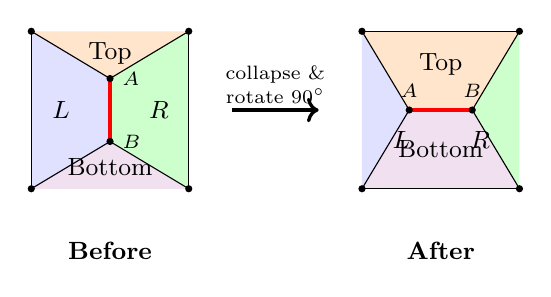
\begin{tikzpicture}[scale=1.0, every node/.style={font=\small}]
  % ---------- BEFORE ----------
  \begin{scope}
    \coordinate (P1) at (-1,1);
    \coordinate (P2) at (1,1);
    \coordinate (P3) at (1,-1);
    \coordinate (P4) at (-1,-1);
    \coordinate (A) at (0,0.4);
    \coordinate (B) at (0,-0.4);
    \fill[blue!12] (P1) -- (A) -- (B) -- (P4) -- cycle;
    \fill[green!20] (P2) -- (A) -- (B) -- (P3) -- cycle;
    \fill[orange!20] (P1) -- (A) -- (P2) -- cycle;
    \fill[violet!12] (P4) -- (B) -- (P3) -- cycle;
    \draw (P1)--(A)--(P2);
    \draw (P4)--(B)--(P3);
    \draw (P1)--(P4);
    \draw (P2)--(P3);
    \draw[red,very thick] (A)--(B);
    \foreach \p in {P1,P2,P3,P4,A,B} \fill (\p) circle (1.3pt);
    \node at (-0.62,0) {$L$};
    \node at (0.62,0) {$R$};
    \node at (0,0.72) {Top};
    \node at (0,-0.72) {Bottom};
    \node[right=1pt] at (A) {\scriptsize$A$};
    \node[right=1pt] at (B) {\scriptsize$B$};
    \node[below] at (0,-1.55) {\textbf{Before}};
  \end{scope}
  % ---------- ARROW ----------
  \draw[->,very thick] (1.55,0) -- (2.65,0);
  \node[align=center] at (2.1,0.32) {\scriptsize collapse \&\\[-2pt]\scriptsize rotate $90^\circ$};
  % ---------- AFTER ----------
  \begin{scope}[xshift=4.2cm]
    \coordinate (P1) at (-1,1);
    \coordinate (P2) at (1,1);
    \coordinate (P3) at (1,-1);
    \coordinate (P4) at (-1,-1);
    \coordinate (C) at (-0.4,0);
    \coordinate (D) at (0.4,0);
    \fill[blue!12] (P1) -- (C) -- (P4) -- cycle;
    \fill[green!20] (P2) -- (D) -- (P3) -- cycle;
    \fill[orange!20] (P1) -- (C) -- (D) -- (P2) -- cycle;
    \fill[violet!12] (P4) -- (C) -- (D) -- (P3) -- cycle;
    \draw (P1)--(C)--(P4);
    \draw (P2)--(D)--(P3);
    \draw (P1)--(P2);
    \draw (P4)--(P3);
    \draw[red,very thick] (C)--(D);
    \foreach \p in {P1,P2,P3,P4,C,D} \fill (\p) circle (1.3pt);
    \node at (-0.5,-0.38) {$L$};
    \node at (0.5,-0.38) {$R$};
    \node at (0,0.58) {Top};
    \node at (0,-0.5) {Bottom};
    \node[above=1pt] at (C) {\scriptsize$A$};
    \node[above=1pt] at (D) {\scriptsize$B$};
    \node[below] at (0,-1.55) {\textbf{After}};
  \end{scope}
\end{tikzpicture}
\caption{The T1 neighbor-exchange transition. \emph{Before}: vertices $A,B$ are
joined by a short edge (\textcolor{red}{red}), shared by the two ``losing'' cells $L,R$;
the two ``gaining'' cells Top, Bottom each touch only one endpoint. \emph{After}: the
edge has collapsed and re-expanded rotated $90^\circ$ --- $L,R$ each drop to one fewer
vertex and no longer touch each other, while Top and Bottom each gain a vertex and
become the new neighboring pair, now sharing the (still red) edge $A$--$B$.}
\label{fig:t1}
\end{figure}

The geometric core (collapse-and-rotate) is short enough to show directly:
\begin{lstlisting}[caption={T1 core: rotating the collapsing edge by $90^\circ$ about
its own midpoint (from \texttt{T1\_swap.f90}). \texttt{scaling\_factor} re-expands the
new edge back out to (at least) the minimum length.}]
scaling_factor = 2.0d0 * min_d_T1 / len_d_T1

call PerpendicularBisector2(OldX, OldY, scaling_factor, NewX, NewY)

v(1, inn(verNoT1,     cellNoT1)) = NewX(2)
v(1, inn(verNoNextT1, cellNoT1)) = NewX(1)
v(2, inn(verNoT1,     cellNoT1)) = NewY(2)
v(2, inn(verNoNextT1, cellNoT1)) = NewY(1)
\end{lstlisting}

\subsection{T2 transition (cell extrusion)}
\textit{Subroutines: \texttt{Do\_T2} (candidate search and guards); \texttt{T2\_core}
(the extrusion itself).}

Any 3-vertex (triangular) cell is a candidate once its area drops below a threshold
$A_{T2}$ (\texttt{min\_area\_T2}) --- geometrically, a cell that has been squeezed down
to (nearly) a point. Physically this is cell extrusion/elimination, as seen for
apoptotic or heavily-compressed cells being pushed out of a real epithelial layer
(Figure~\ref{fig:t2}).
\begin{enumerate}[label=(\arabic*)]
  \item Scan every 3-vertex cell for area below $A_{T2}$; pick one candidate at random.
  \item Collapse its three vertices to their common centroid, which becomes the new
  position of one surviving vertex; the other two vertices are removed.
  \item Every neighboring cell that touched the extruded triangle is stitched back
  together directly across the resulting gap: a neighbor that only touched one corner
  simply loses that one vertex, while a neighbor that shared a full edge (or the whole
  triangle) has its two flanking edges merged onto the single surviving centroid
  vertex.
  \item The extruded cell itself is deleted from the cell list (every higher-indexed
  cell, and its Rho, ROCK, Myosin, and cell-identity data, shifts down by one).
  \item \textbf{Guard}: as with T1, reject the whole event if it would leave any
  neighboring cell with fewer than 3 vertices.
\end{enumerate}

\begin{figure}[htbp]
\centering
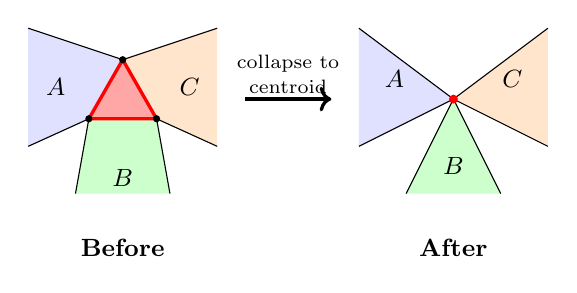
\begin{tikzpicture}[scale=1.0, every node/.style={font=\small}]
  % ---------- BEFORE ----------
  \begin{scope}
    \coordinate (V1) at (0,0.5);
    \coordinate (V2) at (-0.43,-0.25);
    \coordinate (V3) at (0.43,-0.25);
    \coordinate (OA1) at (-1.2,0.9);
    \coordinate (OA2) at (-1.2,-0.6);
    \coordinate (OB1) at (-0.6,-1.2);
    \coordinate (OB2) at (0.6,-1.2);
    \coordinate (OC1) at (1.2,-0.6);
    \coordinate (OC2) at (1.2,0.9);
    \fill[blue!12] (OA1) -- (V1) -- (V2) -- (OA2) -- cycle;
    \fill[green!20] (OB1) -- (V2) -- (V3) -- (OB2) -- cycle;
    \fill[orange!20] (OC1) -- (V3) -- (V1) -- (OC2) -- cycle;
    \fill[red!35] (V1) -- (V2) -- (V3) -- cycle;
    \draw (OA1)--(V1)--(V2)--(OA2);
    \draw (OB1)--(V2)--(V3)--(OB2);
    \draw (OC1)--(V3)--(V1)--(OC2);
    \draw[red,very thick] (V1)--(V2)--(V3)--cycle;
    \foreach \p in {V1,V2,V3} \fill (\p) circle (1.3pt);
    \node at (-0.85,0.15) {$A$};
    \node at (0,-1.0) {$B$};
    \node at (0.85,0.15) {$C$};
    \node[below] at (0,-1.65) {\textbf{Before}};
  \end{scope}
  % ---------- ARROW ----------
  \draw[->,very thick] (1.55,0) -- (2.65,0);
  \node[align=center] at (2.1,0.32) {\scriptsize collapse to\\[-2pt]\scriptsize centroid};
  % ---------- AFTER ----------
  \begin{scope}[xshift=4.2cm]
    \coordinate (M) at (0,0);
    \coordinate (OA1) at (-1.2,0.9);
    \coordinate (OA2) at (-1.2,-0.6);
    \coordinate (OB1) at (-0.6,-1.2);
    \coordinate (OB2) at (0.6,-1.2);
    \coordinate (OC1) at (1.2,-0.6);
    \coordinate (OC2) at (1.2,0.9);
    \fill[blue!12] (OA1) -- (M) -- (OA2) -- cycle;
    \fill[green!20] (OB1) -- (M) -- (OB2) -- cycle;
    \fill[orange!20] (OC1) -- (M) -- (OC2) -- cycle;
    \draw (OA1)--(M)--(OA2);
    \draw (OB1)--(M)--(OB2);
    \draw (OC1)--(M)--(OC2);
    \fill[red] (M) circle (1.6pt);
    \node at (-0.75,0.25) {$A$};
    \node at (0,-0.85) {$B$};
    \node at (0.75,0.25) {$C$};
    \node[below] at (0,-1.65) {\textbf{After}};
  \end{scope}
\end{tikzpicture}
\caption{The T2 extrusion transition. \emph{Before}: a shrinking triangular cell
(\textcolor{red}{red}) with neighbors $A,B,C$ each sharing one of its three edges.
\emph{After}: the triangle has collapsed to its centroid $M$ (\textcolor{red}{red
dot}), which becomes the new shared vertex; $A,B,C$ each lose one vertex and now meet
directly at $M$, a single three-way junction where the cell used to be.}
\label{fig:t2}
\end{figure}

\begin{lstlisting}[caption={T2 core: collapsing the extruded triangle to its centroid
(from \texttt{T2\_swap.f90}).}]
VcmX = sum(vx) / size(vx)
VcmY = sum(vy) / size(vy)

v(1, inn(1,cellNoT2)) = VcmX
v(2, inn(1,cellNoT2)) = VcmY
verNoT2 = inn(1,cellNoT2)   ! this single surviving vertex replaces
                            ! the whole extruded triangle everywhere
\end{lstlisting}

\subsection{Cell division}
\label{sec:division}
\textit{Subroutines: \texttt{Do\_Proliferation} (candidate loop, falling through to
the next candidate on failure); \texttt{Find\_Proliferation} (candidate search);
\texttt{Proliferation\_Core} (the split itself).}

A cell whose area exceeds a threshold $A_{\mathrm{div}}$ (\texttt{area\_0}) is a
division candidate (Figure~\ref{fig:division}).
\begin{enumerate}[label=(\arabic*)]
  \item Compute the cell's \emph{principal axis} --- the direction of greatest
  elongation, from the eigenvectors of its own vertex-position second-moment (inertia)
  tensor about its centroid --- and extend it out to the cell's own extremal
  projections along that direction.
  \item Find where the \emph{perpendicular bisector} of that axis crosses the cell's
  boundary: generically exactly two edges. Insert one brand-new vertex at each
  crossing.
  \item Split the (now vertex-augmented) polygon into two daughter polygons along the
  chord joining the two new vertices, each keeping its share of the original vertex
  list plus both new vertices.
  \item The (up to) two neighboring cells whose edges were cut by this chord also gain
  one new vertex apiece, so their own boundary stays a consistent, gap-free polygon
  after the split.
  \item Every modified polygon (both daughters, both neighbors) is independently
  re-sorted into a consistent, uniquely-defined vertex order (clockwise, starting from
  its own lowest-$x$ vertex) about its own centroid.
  \item One daughter keeps the mother cell's index; the other is appended as a new cell
  at the end of the cell list. Each of the two new vertices inherits the (linearly
  interpolated) motility of the two mother-cell vertices whose edge it split.
  \item \textbf{Guards}: the whole division is skipped cleanly (never partially
  applied) if the bisector fails to cross exactly two edges, if a cut edge lies on the
  tissue's free outer boundary (no second neighboring cell exists to update), if any
  resulting polygon would be degenerate, or if the pre-reserved vertex/cell array
  capacity would be exceeded.
\end{enumerate}

\begin{figure}[htbp]
\centering
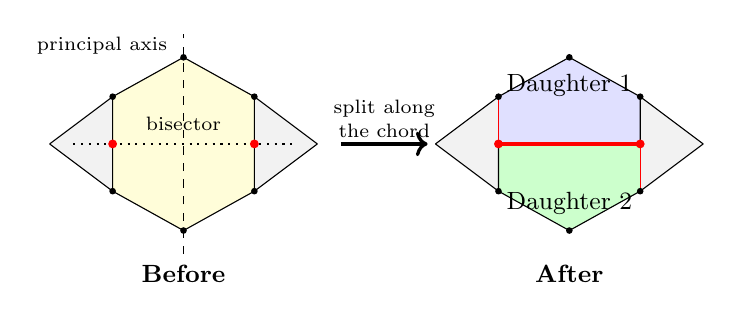
\begin{tikzpicture}[scale=1.0, every node/.style={font=\small}]
  % ---------- BEFORE ----------
  \begin{scope}
    \coordinate (M1) at (0.9,0.6);
    \coordinate (M2) at (0,1.1);
    \coordinate (M3) at (-0.9,0.6);
    \coordinate (M4) at (-0.9,-0.6);
    \coordinate (M5) at (0,-1.1);
    \coordinate (M6) at (0.9,-0.6);
    \coordinate (X1) at (-0.9,0);
    \coordinate (X2) at (0.9,0);
    \coordinate (NLo) at (-1.7,0);
    \coordinate (NRo) at (1.7,0);
    \fill[yellow!15] (M1)--(M2)--(M3)--(M4)--(M5)--(M6)--cycle;
    \fill[gray!10] (NLo)--(M3)--(M4)--cycle;
    \fill[gray!10] (NRo)--(M6)--(M1)--cycle;
    \draw[dashed] (0,-1.4) -- (0,1.4);
    \draw[dotted,thick] (-1.4,0) -- (1.4,0);
    \draw (M1)--(M2)--(M3)--(M4)--(M5)--(M6)--cycle;
    \draw (NLo)--(M3); \draw (NLo)--(M4);
    \draw (NRo)--(M6); \draw (NRo)--(M1);
    \foreach \p in {M1,M2,M3,M4,M5,M6} \fill (\p) circle (1.2pt);
    \fill[red] (X1) circle (1.6pt);
    \fill[red] (X2) circle (1.6pt);
    \node[left=1pt] at (-0.05,1.25) {\scriptsize principal axis};
    \node[above] at (0,0.05) {\scriptsize bisector};
    \node at (0,-1.65) {\textbf{Before}};
  \end{scope}
  % ---------- ARROW ----------
  \draw[->,very thick] (2.0,0) -- (3.1,0);
  \node[align=center] at (2.55,0.32) {\scriptsize split along\\[-2pt]\scriptsize the chord};
  % ---------- AFTER ----------
  \begin{scope}[xshift=4.9cm]
    \coordinate (M1) at (0.9,0.6);
    \coordinate (M2) at (0,1.1);
    \coordinate (M3) at (-0.9,0.6);
    \coordinate (M4) at (-0.9,-0.6);
    \coordinate (M5) at (0,-1.1);
    \coordinate (M6) at (0.9,-0.6);
    \coordinate (X1) at (-0.9,0);
    \coordinate (X2) at (0.9,0);
    \coordinate (NLo) at (-1.7,0);
    \coordinate (NRo) at (1.7,0);
    \fill[blue!12] (X2)--(M1)--(M2)--(M3)--(X1)--cycle;
    \fill[green!20] (X1)--(M4)--(M5)--(M6)--(X2)--cycle;
    \fill[gray!10] (NLo)--(M3)--(X1)--(M4)--cycle;
    \fill[gray!10] (NRo)--(M6)--(X2)--(M1)--cycle;
    \draw (M1)--(M2)--(M3);
    \draw (M4)--(M5)--(M6);
    \draw[red,very thick] (X1)--(X2);
    \draw (NLo)--(M3); \draw[red] (M3)--(X1); \draw (X1)--(M4)--(NLo);
    \draw (NRo)--(M6); \draw[red] (M6)--(X2); \draw (X2)--(M1)--(NRo);
    \foreach \p in {M1,M2,M3,M4,M5,M6} \fill (\p) circle (1.2pt);
    \fill[red] (X1) circle (1.6pt);
    \fill[red] (X2) circle (1.6pt);
    \node at (0,0.75) {Daughter 1};
    \node at (0,-0.75) {Daughter 2};
    \node at (0,-1.65) {\textbf{After}};
  \end{scope}
\end{tikzpicture}
\caption{Cell division. \emph{Before}: the mother cell (yellow) with its principal
axis (dashed) and the perpendicular bisector (dotted) crossing two opposite edges at
$X_1,X_2$ (\textcolor{red}{red dots}); shaded grey are the two flanking neighbor cells
that will each gain a vertex. \emph{After}: the mother cell has split into two
daughters sharing the new chord $X_1$--$X_2$ (\textcolor{red}{red}), and each flanking
neighbor's boundary now includes the corresponding new vertex (\textcolor{red}{red}
segment), keeping the tiling gap-free.}
\label{fig:division}
\end{figure}

\begin{lstlisting}[caption={The division geometry, at a glance (from
\texttt{Proliferation.f90}/\texttt{Geometry.f90}): principal axis, its perpendicular
bisector's two crossing points, then the actual split.}]
call Find_Principle_Axis(vx, vy, nn, x1, y1, x2, y2)

call Find_Bisector_Intersections(vx, vy, nn, x1, y1, x2, y2, &
     x_intersection, y_intersection, n_intersections, inn(1:nn,ic), ic, idx_pair)

if (n_intersections == 2) then
  call Proliferation_Core(ic, Nc, v, inn, num, ..., &
       x_intersection, y_intersection, idx_pair, division_success)
end if
\end{lstlisting}
As a known, deliberate limitation (documented directly alongside the code): the
Rho/ROCK/Myosin chemical state and the cell-identity label are \emph{not} currently
propagated from mother to daughter cell --- only per-vertex motility is.

%========================================================================
\section{Periodic boundary conditions}
\label{sec:pbc}
%========================================================================

Simulating a genuinely bulk, edge-free piece of tissue requires two things: an initial
mesh that is actually topologically periodic (a torus, not just a bounded box), and a
runtime that respects that periodicity in every geometric calculation.

\subsection{Building a periodic mesh}
\textit{Program: \texttt{Generate\_Initial\_Mesh} (\texttt{Generate\_Initial\_Mesh.f90}),
a standalone executable, run once before \texttt{vertexmain.exe}.}

The free-boundary mesh generator already surrounds the real lattice with 8 ``ghost''
copies of every seed point, offset by $(\pm L_x,0)$, $(0,\pm L_y)$ and the four diagonal
combinations, purely so that edge cells have something to clip their Voronoi polygon
against instead of extending to infinity --- but this alone does \emph{not} connect
opposite edges of the box: a vertex on the left edge and its Voronoi counterpart on the
right edge are still two entirely separate, unconnected vertices. True periodicity adds
one further pass: because the ghost tiling sits at \emph{exactly} $\pm L_x,\pm L_y$, any
two vertices near opposite edges of the box whose raw coordinates differ by exactly one
of those offsets are the very same physical point, independently computed twice by two
different cells. These pairs are found and merged into a single shared vertex ID via a
union-find data structure:
\begin{lstlisting}[caption={The core periodic-identification test (from
\texttt{Generate\_Initial\_Mesh.f90}): two candidate vertices are the same physical
point, seen from opposite sides of the box, if some one of the 8 lattice-period
shifts brings them within numerical tolerance of each other.}]
shiftx = (/ -Lx_box, Lx_box, 0.0d0, 0.0d0, -Lx_box, -Lx_box, Lx_box, Lx_box /)
shifty = (/ 0.0d0, 0.0d0, -Ly_box, Ly_box, -Ly_box, Ly_box, -Ly_box, Ly_box /)

do s = 1, 8
   dx = gx(j1) + shiftx(s) - gx(j2)
   dy = gy(j1) + shifty(s) - gy(j2)
   if (dx*dx + dy*dy <= eps*eps) then
      call union_vertices(remap, j1, j2, did_union)   ! merge j1 and j2's vertex IDs
      exit
   end if
end do
\end{lstlisting}
After this pass, every vertex is checked to have degree exactly 3 (touched by exactly 3
cells, with no free-boundary exceptions at all) --- the program refuses to proceed if
it ever finds one that doesn't, rather than silently shipping a mesh with a hidden free
edge. The resulting mesh has Euler characteristic $V - E + F = 0$, the topological
signature of a torus (a bounded, disk-like mesh instead has $V-E+F\approx 2$).

\subsection{Runtime handling: wrap, and gather-and-unwrap}
\textit{Subroutines (all three in \texttt{Geometry.f90}):}
\texttt{Wrap\_Position},
\texttt{Unwrap\_\allowbreak Relative},
\texttt{Gather\_\allowbreak Cell\_\allowbreak Vertices\_\allowbreak PBC}.

Two separate rules keep the running simulation consistent with this periodic topology.
\begin{itemize}
  \item \textbf{Wrapping.} After every step that can move a vertex, its position is
  folded back into one canonical box $[0,L_x)\times[0,L_y)$ by simple modular
  arithmetic. This only changes how a position is \emph{reported}, never any physical
  distance or force.
  \item \textbf{Gather-and-unwrap (minimum image).} Any calculation that needs several
  vertices of the \emph{same} cell together --- area, perimeter, its centroid, the
  force gradients of Section~\ref{sec:force}, the principal axis for division, the
  stress tensor of Section~\ref{sec:stress} --- cannot safely use the vertices' raw,
  independently-wrapped coordinates: a cell that happens to straddle the box edge has
  some vertices stored near $x=0$ and others near $x=L_x$, even though physically all
  of them sit close together (Figure~\ref{fig:pbc}). The fix, applied uniformly
  everywhere in the code such a cell-vertex list is gathered: take the cell's first
  vertex as a local reference, and shift every other vertex of that cell by whichever
  whole multiple of the box size brings it closest to that reference (the
  minimum-image convention). This never changes any real distance or angle inside the
  cell --- it only re-expresses the same physical shape without an artificial
  box-spanning jump.
\end{itemize}

\begin{figure}[htbp]
\centering
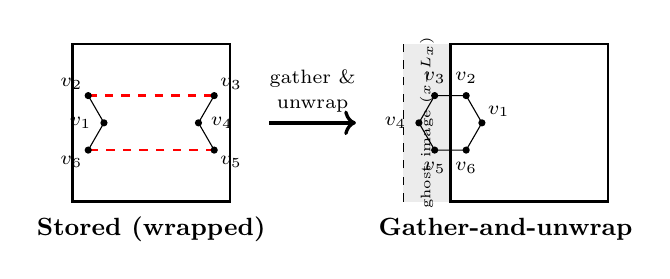
\begin{tikzpicture}[scale=1.0, every node/.style={font=\small}]
  % ---------- PANEL 1: stored / wrapped (wired artifact) ----------
  \begin{scope}
    \draw[thick] (0,0) rectangle (2,2);
    \coordinate (v1) at (0.4,1.0);
    \coordinate (v2) at (0.2,1.346);
    \coordinate (v3) at (1.8,1.346);
    \coordinate (v4) at (1.6,1.0);
    \coordinate (v5) at (1.8,0.654);
    \coordinate (v6) at (0.2,0.654);
    \draw (v1)--(v2);
    \draw[red,dashed,thick] (v2)--(v3);
    \draw (v3)--(v4)--(v5);
    \draw[red,dashed,thick] (v5)--(v6);
    \draw (v6)--(v1);
    \foreach \p in {v1,v2,v3,v4,v5,v6} \fill (\p) circle (1.3pt);
    \node[left=1pt] at (v1) {\scriptsize$v_1$};
    \node[above left=-2pt] at (v2) {\scriptsize$v_2$};
    \node[above right=-2pt] at (v3) {\scriptsize$v_3$};
    \node[right=1pt] at (v4) {\scriptsize$v_4$};
    \node[below right=-2pt] at (v5) {\scriptsize$v_5$};
    \node[below left=-2pt] at (v6) {\scriptsize$v_6$};
    \node at (1,-0.35) {\textbf{Stored (wrapped)}};
  \end{scope}
  % ---------- ARROW ----------
  \draw[->,very thick] (2.5,1) -- (3.6,1);
  \node[align=center] at (3.05,1.4) {\scriptsize gather \&\\[-2pt]\scriptsize unwrap};
  % ---------- PANEL 2: gather-and-unwrap ----------
  \begin{scope}[xshift=4.8cm]
    \fill[gray!15] (-0.6,0) rectangle (0,2);
    \draw[thick] (0,0) rectangle (2,2);
    \draw[dashed] (-0.6,0) -- (-0.6,2);
    \coordinate (v1) at (0.4,1.0);
    \coordinate (v2) at (0.2,1.346);
    \coordinate (v3) at (-0.2,1.346);
    \coordinate (v4) at (-0.4,1.0);
    \coordinate (v5) at (-0.2,0.654);
    \coordinate (v6) at (0.2,0.654);
    \draw (v1)--(v2)--(v3)--(v4)--(v5)--(v6)--cycle;
    \foreach \p in {v1,v2,v3,v4,v5,v6} \fill (\p) circle (1.3pt);
    \node[above right=-2pt] at (v1) {\scriptsize$v_1$};
    \node[above=1pt] at (v2) {\scriptsize$v_2$};
    \node[above=1pt] at (v3) {\scriptsize$v_3$};
    \node[left=1pt] at (v4) {\scriptsize$v_4$};
    \node[below=1pt] at (v5) {\scriptsize$v_5$};
    \node[below=1pt] at (v6) {\scriptsize$v_6$};
    \node[rotate=90] at (-0.3,1.0) {\tiny ghost image ($x{-}L_x$)};
    \node at (0.7,-0.35) {\textbf{Gather-and-unwrap}};
  \end{scope}
\end{tikzpicture}
\caption{The gather-and-unwrap fix, for a cell straddling the box's periodic edge
($L_x=L_y=2$ here). \emph{Left}: the cell's 6 vertices as actually stored --- $v_1,v_2,v_6$
near $x=0$, $v_3,v_4,v_5$ wrapped to near $x=L_x$ --- naively connecting consecutive
vertices produces two long, spurious edges (\textcolor{red}{red dashed}) spanning the
whole box. \emph{Right}: the same 6 vertices, each shifted by whichever multiple of
$L_x$ brings it closest to the reference vertex $v_1$; $v_3,v_4,v_5$ now sit in the
box's left periodic image (shaded), and the reconstructed hexagon is short-edged and
compact everywhere, straddling the boundary exactly as the physical cell does.}
\label{fig:pbc}
\end{figure}

The entire mechanism is three short routines, used as a drop-in replacement for the
plain ``read this cell's vertices'' pattern everywhere in the codebase (energy, force,
T1, T2, division, stress) --- and an exact no-op, byte-identical to the original code,
whenever periodic boundaries are switched off:
\begin{lstlisting}[caption={The complete PBC machinery (from \texttt{Geometry.f90}).
\texttt{Gather\_\allowbreak Cell\_\allowbreak Vertices\_\allowbreak PBC} is called everywhere a cell's vertex list is
needed, in place of the old raw \texttt{v(1,inn(1:nn,ic))} pattern.}]
subroutine Wrap_Position(x, y)
  if (.not. if_PBC) return
  x = modulo(x, Lx_box)
  y = modulo(y, Ly_box)
end subroutine

subroutine Unwrap_Relative(x_ref, y_ref, x, y)
  ! replace (x,y) with whichever periodic image of itself is closest to (x_ref,y_ref)
  if (.not. if_PBC) return
  dx = x - x_ref;  dx = dx - Lx_box * dnint(dx / Lx_box)
  dy = y - y_ref;  dy = dy - Ly_box * dnint(dy / Ly_box)
  x = x_ref + dx;  y = y_ref + dy
end subroutine

subroutine Gather_Cell_Vertices_PBC(ids, nn, vx, vy)
  vx = v(1, ids(1:nn));  vy = v(2, ids(1:nn))
  if (.not. if_PBC) return
  do i = 2, nn
    call Unwrap_Relative(vx(1), vy(1), vx(i), vy(i))   ! unwrap every vertex after
  end do                                               ! the first, relative to it
end subroutine
\end{lstlisting}
A few global quantities have no well-defined periodic analogue at all and are handled
by simplifying rather than patching: the free-boundary stress calculation restricts
itself to an inner disk around the tissue's center of mass purely to avoid edge
artifacts (Section~\ref{sec:stress}) --- under full periodicity there is no edge to
avoid, and no well-defined single ``center of mass'' on a torus either (exactly like
averaging angles), so every cell is simply included instead of attempting to fix the
disk-selection logic itself.

\section{From equations to code: a guided tour of the implementation}
\label{sec:code-tour}

Everything above this point describes the model in the language of physics: energies,
forces, stochastic rules, topological rearrangements. This section switches to the
other side of the same coin --- the actual Fortran program that turns those equations
into a running simulation, file by file, subroutine by subroutine. Nothing here is a
different model; it is the same equations, just written as code instead of
mathematics. The goal is that a reader with no Fortran background, but who has read
the sections above, can open any of these source files and know what they are looking
at and why it is written the way it is.

A short reading guide before diving in: Fortran organizes code into \emph{modules}
(roughly, a file that bundles together a set of related \emph{subroutines} and
\emph{functions}, plus the shared variables they all use) and, for this codebase, one
\emph{program} --- the single entry point where execution actually begins, analogous to
\texttt{main()} in C. A subroutine is a named, reusable block of code that performs an
action (it can modify its inputs, print things, write files); a function is the same
idea but always returns a single value. ``\texttt{call Foo}'' simply means ``go run
the block of code named \texttt{Foo} now, then come back here when it's done.'' The
codebase is deliberately organized so that each file owns one conceptual job: geometry,
forces, topological events, and so on --- the map below shows how they fit together.

\subsection{Two programs, one shared codebase}

There are, in fact, \emph{two} separate compiled programs sharing these source files:

\begin{itemize}[leftmargin=1.5em]
  \item \textbf{\texttt{generate\_initial\_mesh}} (\texttt{Generate\_Initial\_Mesh.f90}) ---
  run once, before any simulation, to build the initial tissue geometry (Section~\ref{sec:codegenmesh}).
  It reads a small parameter file (\texttt{para\_MeshGen.dat}) and writes four data files
  describing the mesh: \texttt{v\_in.dat} (vertex positions), \texttt{inn\_in.dat}
  (which vertices belong to which cell), \texttt{num\_in.dat} (how many vertices each
  cell has), and \texttt{para\_MeshDims.dat} (the array sizes needed to read the other
  three).
  \item \textbf{\texttt{vertexmain}} (\texttt{vertexmain.f90}) --- the actual physics
  simulation described in every earlier section of this document. It reads those same
  four mesh files (plus its own much longer parameter file, \texttt{para\_Simulation.dat}),
  then runs the timestep loop until it has produced a full trajectory.
\end{itemize}

These two programs never run at the same time and do not call each other directly ---
the mesh generator's job ends the moment it has written its four files to disk; the
main program's job begins by reading them back in. They are connected only through
those files, which is why Figure~\ref{fig:master-map} draws them as two separate boxes
joined by a single arrow.

\subsection{Master map of the codebase}

Figure~\ref{fig:master-map} is the master map: every box is a subroutine (or a phase of
one), and an arrow from box A to box B means ``A calls B.'' The left branch is the mesh
generator (one straight sequence of phases, described fully in
Section~\ref{sec:codegenmesh}); the right branch is the main simulation's setup followed
by its repeating per-timestep loop. Each named phase in the loop is one row of
Table~\ref{tab:module-map}, which says which file/module actually implements it --- use
that table as the index into the rest of this section.

\begin{figure}[htbp]
\centering
\resizebox{\textwidth}{!}{%
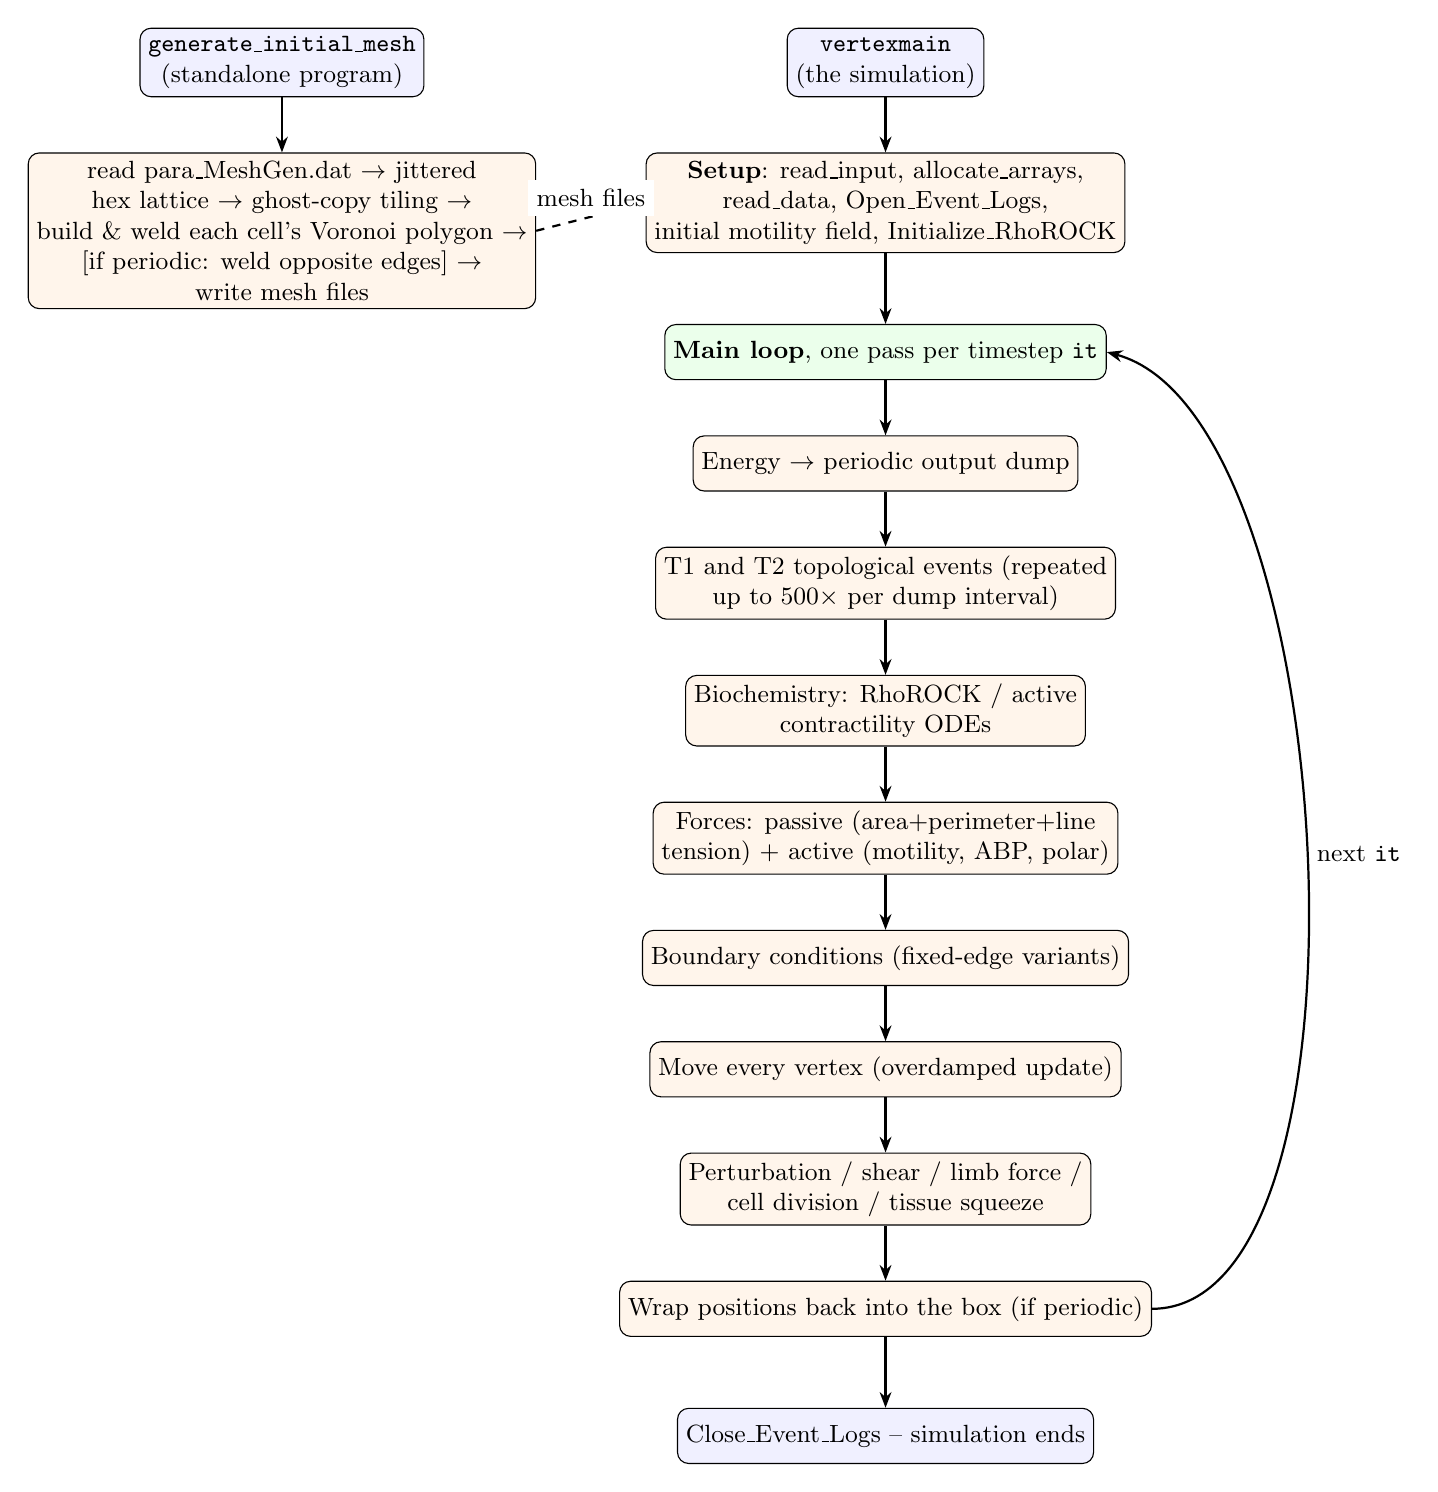
\begin{tikzpicture}[
  node distance=7mm and 12mm,
  every node/.style={font=\small},
  box/.style={draw, rounded corners, fill=blue!6, align=center, minimum height=7mm, inner sep=3pt},
  phase/.style={draw, rounded corners, fill=orange!8, align=center, minimum height=7mm, inner sep=3pt},
  loopbox/.style={draw, rounded corners, fill=green!8, align=center, minimum height=7mm, inner sep=3pt},
  arr/.style={-{Stealth[length=2mm]}, thick},
]

 % ---- Left branch: mesh generator ----
 \node[box] (gen) {\texttt{generate\_initial\_mesh}\\(standalone program)};
 \node[phase, below=of gen] (genphases) {read para\_MeshGen.dat $\to$ jittered\\
   hex lattice $\to$ ghost-copy tiling $\to$\\
   build \& weld each cell's Voronoi polygon $\to$\\
   {[}if periodic: weld opposite edges{]} $\to$\\
   write mesh files};

 \node[box, right=46mm of gen] (main) {\texttt{vertexmain}\\(the simulation)};

 \node[phase, below=of main] (setup) {\textbf{Setup}: read\_input, allocate\_arrays,\\
   read\_data, Open\_Event\_Logs,\\
   initial motility field, Initialize\_RhoROCK};

 \node[loopbox, below=of setup, yshift=-2mm] (loopstart) {\textbf{Main loop}, one pass per timestep \texttt{it}};

 \node[phase, below=of loopstart] (energy) {Energy $\to$ periodic output dump};
 \node[phase, below=of energy] (topo) {T1 and T2 topological events (repeated\\
   up to 500$\times$ per dump interval)};
 \node[phase, below=of topo] (biochem) {Biochemistry: RhoROCK / active\\
   contractility ODEs};
 \node[phase, below=of biochem] (force) {Forces: passive (area+perimeter+line\\
   tension) + active (motility, ABP, polar)};
 \node[phase, below=of force] (bc) {Boundary conditions (fixed-edge variants)};
 \node[phase, below=of bc] (move) {Move every vertex (overdamped update)};
 \node[phase, below=of move] (extra) {Perturbation / shear / limb force /\\
   cell division / tissue squeeze};
 \node[phase, below=of extra] (wrap) {Wrap positions back into the box (if periodic)};

 \node[box, below=of wrap, yshift=-2mm] (close) {Close\_Event\_Logs -- simulation ends};

 \draw[arr] (gen) -- (genphases);
 \draw[arr] (main) -- (setup);
 \draw[arr, dashed] (genphases.east) -- node[above, midway, fill=white]{mesh files} (setup.west);
 \draw[arr] (setup) -- (loopstart);
 \draw[arr] (loopstart) -- (energy);
 \draw[arr] (energy) -- (topo);
 \draw[arr] (topo) -- (biochem);
 \draw[arr] (biochem) -- (force);
 \draw[arr] (force) -- (bc);
 \draw[arr] (bc) -- (move);
 \draw[arr] (move) -- (extra);
 \draw[arr] (extra) -- (wrap);
 \draw[arr] (wrap) -- (close);
 \draw[arr] (wrap.east) .. controls +(30mm,0) and +(30mm,-8mm) .. node[right, midway]{next \texttt{it}} (loopstart.east);

\end{tikzpicture}
}
\caption{Master map of the codebase. Left: the standalone mesh generator, run once.
Right: the main simulation's setup phase followed by its repeating timestep loop ---
the green loop-back arrow on the right is the ``do it = 1, totT'' loop in
\texttt{vertexmain.f90}. Every phase box names the actual subroutine(s) behind it;
Table~\ref{tab:module-map} maps each phase to the file/module that implements it and
the section of this document where it is documented in detail.}
\label{fig:master-map}
\end{figure}

\begin{table}[htbp]
\centering
\small
\begin{tabular}{@{}p{0.30\textwidth}p{0.28\textwidth}p{0.34\textwidth}@{}}
\toprule
\textbf{Phase (Fig.~\ref{fig:master-map})} & \textbf{File / module} & \textbf{Key subroutines} \\
\midrule
Setup (read parameters, allocate, load mesh) & \texttt{allocation.f90} & \texttt{read\_input}, \texttt{allocate\_arrays}, \texttt{read\_data} \\
Energy \& periodic output & \texttt{System\_Info.f90}, \texttt{allocation.f90} & \texttt{Calculate\_Energy}, \texttt{write\_output} \\
T1 / T2 topological events & \texttt{T1\_swap.f90}, \texttt{T2\_swap.f90} & \texttt{Do\_T1}, \texttt{Do\_T2} \\
Biochemistry (Rho/ROCK/Myosin) & \texttt{Force.f90} & \texttt{Solve\_RhoROCK\_Euler/RK4}, \texttt{Solve\_Myosin\_Act\_Contr} \\
Forces (passive + active) & \texttt{Force.f90} & \texttt{Force\_Calculation}, \texttt{Motile\_Force\_Calculation}, \texttt{ABP\_Force\_Calculation}, \texttt{Polar\_Motile\_Force\_Calculation} \\
Boundary conditions & \texttt{Force.f90}, \texttt{Geometry.f90} & \texttt{Apply\_Fixed\_Boundary} and friends, \texttt{Find\_boundary\_dynamic} \\
Shear / perturbation / limb force & \texttt{Stress.f90}, \texttt{Force.f90} & \texttt{ShearTissue}, \texttt{Apply\_perturbation}, \texttt{Apply\_Limb\_Force} \\
Cell division & \texttt{Proliferation.f90}, \texttt{Geometry.f90} & \texttt{Do\_Proliferation}, \texttt{Proliferation\_Core}, \texttt{SplitPolygon} \\
Tissue squeeze & \texttt{Geometry.f90} & \texttt{Squeeze\_Tissue} \\
Geometric primitives (used by everything above) & \texttt{Geometry.f90} & \texttt{CalculateArea}, \texttt{CalculatePerimeter}, PBC helpers \\
Small shared utilities & \texttt{array\_info.f90} & \texttt{find\_unique\_sorted}, \texttt{quicksort\_recursive} \\
Stress tensor & \texttt{Stress.f90} & \texttt{Calculate\_StressTensor} \\
Mesh generation (separate program) & \texttt{Generate\_Initial\_Mesh.f90} & Section~\ref{sec:codegenmesh} \\
\bottomrule
\end{tabular}
\caption{Which file/module implements each phase of Figure~\ref{fig:master-map}, and
which subroutines to look for first.}
\label{tab:module-map}
\end{table}

The sections that follow go through every one of these files, in an order chosen to
read naturally rather than alphabetically: the small shared utility file first
(Section~\ref{sec:codearrayinfo}), then the central bookkeeping module that every other
file leans on (Section~\ref{sec:codealloc}), then geometry, forces, the two topological
events, cell division, and finally the standalone mesh generator. Every subroutine, no
matter how short, gets its own paragraph: its full argument list, what it does and why,
a short code excerpt, and which other routines it calls or is called by.
\subsection{\texttt{array\_info.f90}: two small shared utilities}
\label{sec:codearrayinfo}

This is the smallest file in the codebase: two general-purpose helper routines with no
physics in them at all, used by the T1 and T2 routines (Sections~\ref{sec:codet1},
\ref{sec:codet2}) to turn a messy list of ``every cell that touched vertex X or Y''
into a clean list of unique cells with a count of how many times each one appeared.

\paragraph{\texttt{find\_unique\_sorted} (lines 12--68).}
\textbf{What it does.} Takes a list of cell indices that may contain repeats (e.g.\ ``cell 5
showed up 3 times, cell 12 showed up once''), and returns two shorter lists: the
distinct values, and how many times each one occurred. It works by sorting a copy of
the input first (via \texttt{quicksort\_recursive}, below) --- once sorted, equal values
are automatically next to each other, so a single left-to-right pass can count each run
and split the list into unique values plus their occurrence counts.

\textbf{Inputs/outputs.}
\begin{itemize}[nosep]
  \item input list of cell indices, possibly with repeats (\texttt{temp\_array}) --- in
  \item how many of \texttt{temp\_array}'s entries to actually look at (\texttt{ik}) --- in
  \item the distinct cell indices found, sorted (\texttt{affected}) --- out (allocated inside)
  \item how many times each of those distinct cells appeared (\texttt{occurrences}) --- out (allocated inside)
\end{itemize}

\begin{lstlisting}[caption={The core counting pass of \texttt{find\_unique\_sorted}, after the input has already been sorted.}]
count = 1
do i = 2, n
  if (temp(i) /= temp(i - 1)) count = count + 1
end do
allocate(affected(count), occurrences(count))
! walk the sorted array once more, recording each run's value and length
\end{lstlisting}

\textbf{Calls:} \texttt{quicksort\_recursive}. \textbf{Called by:} \texttt{find\_T1\_Affected}
and \texttt{find\_T2\_Affected} (Sections~\ref{sec:codet1}, \ref{sec:codet2}) --- both use
it to collapse ``every cell touching either endpoint of this edge/triangle'' into the
handful of distinct cells genuinely affected by a T1 or T2 event, plus how many of the
event's vertices each one touches (which is exactly what tells \texttt{T1\_core}/\texttt{T2\_core}
whether a given affected cell is \emph{losing} a vertex or \emph{gaining} one).

\paragraph{\texttt{quicksort\_recursive} (lines 70--111).}
\textbf{What it does.} A textbook recursive quicksort: pick the first element as a
\emph{pivot}, partition the rest of the array so everything smaller ends up on one side
and everything larger on the other, then recursively sort each side the same way. This
is a completely standard, general-purpose sorting algorithm --- nothing here is
specific to vertex models --- included only because \texttt{find\_unique\_sorted} needs
its input sorted before it can count runs.

\textbf{Inputs/outputs.}
\begin{itemize}[nosep]
  \item the array being sorted (\texttt{arr}) --- inout, modified in place
  \item the first index of the region to sort this call (\texttt{left}) --- in
  \item the last index of the region to sort this call (\texttt{right}) --- in
\end{itemize}

\begin{lstlisting}[caption={The partition-and-recurse structure of \texttt{quicksort\_recursive}.}]
if (left >= right) return
pivot = arr(left)
! ... partition arr(left:right) around pivot, ending with pivot at position i ...
call quicksort_recursive(arr, left, i - 1)
call quicksort_recursive(arr, i + 1, right)
\end{lstlisting}

\textbf{Calls:} itself (recursively). \textbf{Called by:} \texttt{find\_unique\_sorted}.
\subsection{\texttt{allocation.f90}: shared state, parameters, and file I/O}
\label{sec:codealloc}

This module is the codebase's ``central nervous system.'' It declares essentially
every array and variable that the rest of the program shares --- the vertex positions,
the cell-to-vertex connectivity, all the physical parameters, all the on/off feature
flags --- and every other file starts with \texttt{use allocation} to get access to
them. It also owns all the file reading and writing: the simulation's parameters, its
starting mesh, and every snapshot written to disk while it runs. Because nearly every
variable named anywhere else in this document (\texttt{v}, \texttt{inn}, \texttt{num},
\texttt{Nc}, \dots) is declared here, this module has no ``physics'' of its own but is
the reason every other file can just start using those names directly.

The key shared arrays declared here, referenced constantly below: the \textbf{vertex
coordinate array} (\texttt{v}), a $2\times$(max vertices) table of every vertex's
$(x,y)$ position; the \textbf{cell-to-vertex connectivity table} (\texttt{inn}), where
column \texttt{ic} lists (in order around the cell) the vertex indices belonging to
cell \texttt{ic}; the \textbf{per-cell vertex count} (\texttt{num}), so \texttt{num(ic)}
says how many of \texttt{inn(:,ic)}'s slots are actually used; and the \textbf{live cell
count} (\texttt{Nc}), the number of cells currently alive (cells $1{:}$\texttt{Nc} are
always the live ones, by convention).

\paragraph{\texttt{read\_input} (lines 222--429).}
\textbf{What it does.} Opens the two parameter files and reads every single simulation
parameter from them, in a fixed order that must exactly match the order the parameter
files list them in (a comment in \texttt{para\_Simulation.dat} itself warns against
reordering one without the other). This includes the mechanical constants ($A_0$,
$\lambda$, $\beta$, $\gamma$, \dots), every feature on/off flag (\texttt{if\_ABP},
\texttt{if\_cell\_division}, \texttt{if\_PBC}, and around fifty more), and the array
sizes needed to know how big the mesh is (read from \texttt{para\_MeshDims.dat}, the
file \texttt{generate\_initial\_mesh} produced). After reading, it does three more
things: (1) it \textbf{nondimensionalizes} $\beta$ and $\gamma$ exactly once here ---
dividing by $\lambda A_0$ and $\lambda A_0^{1.5}$ respectively
--- so every other subroutine that uses them never has to repeat that rescaling itself;
(2) it computes \texttt{summary\_dump\_interval}, a throttle on how often the slowly-growing
summary files (energy, shear stress, T1/T2 counts) get rewritten, chosen so a very long
run doesn't spend most of its time rewriting an ever-larger file; (3) it checks a
handful of flag combinations that don't make physical sense together (e.g.\ periodic
boundaries together with a fixed-edge boundary condition, which has no free edge left
to fix) and stops the program immediately with a clear message if it finds one, rather
than running with a contradictory setup and producing silently wrong results.

\textbf{Inputs/outputs.} Takes no arguments; reads from disk and fills in dozens of
module-level variables directly. The two files it opens: the \textbf{simulation parameter
file} (\texttt{para\_Simulation.dat}, Fortran unit 112) and the \textbf{mesh dimensions
file} (\texttt{para\_MeshDims.dat}, unit 121).

\begin{lstlisting}[caption={A representative slice of \texttt{read\_input}: nondimensionalizing beta/gamma once, and one of several flag-compatibility checks.}]
beta = beta/(lambda*Ao)
gamm = gamm/(lambda*(Ao)**1.5)

if (if_PBC) then
  if (if_Fixed_boundary .or. if_bottom_borders_fixed .or. if_top_borders_fixed) then
    write(*,*) 'read_input: if_PBC is incompatible with if_Fixed_boundary/...'
    stop 1
  end if
end if
\end{lstlisting}

\textbf{Calls:} none. \textbf{Called by:} \texttt{allocate\_arrays} (immediately, as its
very first action, since every array size it allocates depends on values \texttt{read\_input}
just read).

\paragraph{\texttt{allocate\_arrays} (lines 431--530).}
\textbf{What it does.} Reserves memory for every array the simulation will use, sized
according to the dimensions \texttt{read\_input} just loaded --- plus some ``headroom''
built into those sizes (extra cell slots and vertex slots beyond what the starting mesh
needs) so that cell division can later create new cells/vertices without running out of
room. It also sets every array's starting values: forces to zero, the biochemical
fields (Rho, ROCK, Myosin) to zero, and --- importantly --- gives every one of the
starting cells its own permanent, unique \textbf{cell identity label}
(\texttt{cell\_identity}), a string like \texttt{"cell\_17"} that stays attached to that
cell (and, after division, to whichever daughter keeps its slot) for the rest of the
run, no matter how much the mesh reshuffles around it. It also initializes the
\textbf{next available cell-identity number} (\texttt{next\_new\_cell\_id}) to one past
the last starting cell, so that when cell division later needs to hand out a brand-new
label to a daughter cell, it always gets a number nothing has ever used before.

\textbf{Inputs/outputs.} Takes no arguments; everything it produces is one of the large
shared arrays declared at the top of the module (\texttt{v}, \texttt{inn}, \texttt{num},
\texttt{Rho}, \texttt{ROCK}, \texttt{Myosin}, \texttt{cell\_identity}, and around twenty
others), all sized from the dimension variables \texttt{read\_input} filled in
(\texttt{num\_dim}, \texttt{v\_dim1}, \texttt{v\_dim2}, \texttt{inn\_dim1}, \texttt{inn\_dim2}).

\begin{lstlisting}[caption={Giving every starting cell its permanent identity label, and priming the counter for future divisions.}]
cell_identity = 'cell_0'
do iic = 1, Lx*Ly
  write(cell_identity(iic), '(A,I0)') 'cell_', iic
end do
next_new_cell_id = Lx*Ly + 1
\end{lstlisting}

\textbf{Calls:} \texttt{read\_input}. \textbf{Called by:} \texttt{vertexmain} (the main
program), as the second setup step.

\paragraph{\texttt{read\_data} (lines 532--680).}
\textbf{What it does.} Loads the actual starting mesh --- either the freshly generated
one from \texttt{generate\_initial\_mesh} (a fresh run, \texttt{nrun=1}), or a saved
snapshot from partway through a previous run (a restart, \texttt{nrun=2}) --- into the
vertex coordinate array (\texttt{v}), the connectivity table (\texttt{inn}), and the
per-cell vertex count (\texttt{num}). It then derives the live cell count (\texttt{Nc})
directly from \texttt{num} (counting how many cells have a nonzero vertex count) rather
than assuming it equals the original $L_x \times L_y$ lattice size --- important for a
restart taken after cell divisions have already happened. Finally, it runs a sanity
check: it measures how many cells touch each vertex (a properly connected interior
vertex is always touched by exactly 3 cells) and compares that against the
\texttt{if\_PBC} setting, stopping the program with an explanatory message if the mesh
and the periodic-boundary flag disagree with each other (e.g.\ a genuinely periodic
mesh being run as if it had a free edge, which silently corrupts areas and perimeters
for any cell straddling the wrap and would otherwise blow up into \texttt{NaN} a few
steps in without explanation).

\textbf{Inputs/outputs.} Takes no arguments; reads from the mesh files on disk
(\texttt{num\_in.dat}, \texttt{v\_in.dat}, \texttt{inn\_in.dat} for a fresh run, or the
matching \texttt{data/inn\_}\dots\texttt{.dat}/\texttt{v\_}\dots\texttt{.dat}/\texttt{num\_}\dots\texttt{.dat}
snapshot files for a restart) and fills in \texttt{v}, \texttt{inn}, \texttt{num}, and
the \textbf{live cell count} (\texttt{Nc}).

\begin{lstlisting}[caption={Deriving the live cell count from the loaded mesh, and the periodicity sanity check.}]
Nc = count(num /= 0)

! measure how many cells touch each vertex; an interior vertex always has degree 3
deg_check(inn(ll,kk)) = deg_check(inn(ll,kk)) + 1
...
if ((.not. if_PBC) .and. mesh_looks_periodic) then
  write(*,*) 'read_data: STOPPING -- this mesh has ZERO free-boundary vertices ...'
  stop 1
end if
\end{lstlisting}

\textbf{Calls:} none. \textbf{Called by:} \texttt{vertexmain}, right after \texttt{allocate\_arrays}.

\paragraph{\texttt{Open\_Event\_Logs} (lines 682--721).}
\textbf{What it does.} Opens three small output files --- one each for T1 events, T2
events, and cell-division events --- once, right before the simulation starts, and
leaves them open for the whole run. Each of these files is written to incrementally,
one short record per actual event, every time one happens (Sections~\ref{sec:codet1},
\ref{sec:codet2}, \ref{sec:codeprolif}), rather than being rewritten from scratch each
time --- these events are sparse and irregular, so a normal ``rewrite the whole file''
approach used for the regular per-timestep snapshots would be wasteful here.

\textbf{Inputs/outputs.} Takes no arguments. Opens the \textbf{T1-event log file}
(\texttt{data/T1\_events.dat}), the \textbf{T2-event log file}
(\texttt{data/T2\_events.dat}), and the \textbf{division-event log file}
(\texttt{data/Division\_events.dat}) --- each renamed with an \texttt{nrun2\_} prefix for
a restart run, so a restart's log never overwrites the original run's.

\begin{lstlisting}[caption={Opening the three event logs, once, before the timestep loop begins.}]
open(unit=iunit_T1events, file=fname_T1events, form='unformatted', status='replace')
open(unit=iunit_T2events, file=fname_T2events, form='unformatted', status='replace')
open(unit=iunit_Divisionevents, file=fname_Divisionevents, form='unformatted', status='replace')
\end{lstlisting}

\textbf{Calls:} none. \textbf{Called by:} \texttt{vertexmain}, once, right after
\texttt{read\_data}.

\paragraph{\texttt{CellIdNum} (lines 723--738, a \emph{function}, not a subroutine).}
\textbf{What it does.} A tiny text-parsing helper: given a cell's identity label (a
string like \texttt{"cell\_17"}), it extracts and returns just the number
(\texttt{17.0d0}) as a plain floating-point value. This exists purely so the compact
binary event logs above can store a cell's identity as one number instead of the whole
padded text string --- about half the file size for the same information, since the
number can always be turned back into the string \texttt{"cell\_"} $+$ the number on
the reading (MATLAB) side. A cell identity that doesn't parse as expected (the
\texttt{"cell\_0"} placeholder used for an empty slot) returns \texttt{0.0}, matching
this codebase's usual convention that zero means ``nothing here.''

\textbf{Inputs/outputs.}
\begin{itemize}[nosep]
  \item the identity label to parse (\texttt{id\_str}) --- in
  \item \emph{(function result)} the numeric suffix, or \texttt{0.0d0} if it can't be parsed (\texttt{num\_out}) --- out
\end{itemize}

\begin{lstlisting}[caption={The complete body of the \texttt{CellIdNum} function.}]
read(id_str(6:), *, iostat=ios) n
if (ios /= 0) then
  num_out = 0.0d0
else
  num_out = dble(n)
end if
\end{lstlisting}

\textbf{Calls:} none. \textbf{Called by:} \texttt{Do\_T1}, \texttt{Do\_T2}, and
\texttt{Proliferation\_Core} (Sections~\ref{sec:codet1}, \ref{sec:codet2},
\ref{sec:codeprolif}), each time they write a record to one of the three event logs.

\paragraph{\texttt{Close\_Event\_Logs} (lines 740--745).}
\textbf{What it does.} The mirror image of \texttt{Open\_Event\_Logs}: closes the same
three event-log files once, right after the simulation's last timestep, so everything
written to them is safely flushed to disk.

\textbf{Inputs/outputs.} Takes no arguments; no return value.

\begin{lstlisting}[caption={The complete body of \texttt{Close\_Event\_Logs}.}]
close(iunit_T1events)
close(iunit_T2events)
close(iunit_Divisionevents)
\end{lstlisting}

\textbf{Calls:} none. \textbf{Called by:} \texttt{vertexmain}, once, right after the
timestep loop ends.

\paragraph{\texttt{write\_output} (lines 747--892).}
\textbf{What it does.} Writes out a full snapshot of the current simulation state ---
called periodically during the run (Table~\ref{tab:module-map}), not just at the very
end, so a run in progress can already be inspected or plotted. Each call writes: the
connectivity table (\texttt{inn}), the per-cell vertex count (\texttt{num}), the vertex
coordinate array (\texttt{v}), every vertex's force components (\texttt{fxx},
\texttt{fyy}, and their active/random counterparts), the biochemical state
(\texttt{Rho}, \texttt{ROCK}, \texttt{Myosin}), every cell's identity label
(\texttt{cell\_identity}), and the per-vertex motility field (\texttt{mot}) --- each to
its own file, named with the current timestep number so a whole sequence of snapshots
builds up over the run (e.g.\ \texttt{v\_00050000.dat} is the vertex positions at
timestep 50000). It also periodically rewrites four smaller, ever-growing summary
files: the whole-tissue energy, shear stress, and cumulative T1/T2 counts recorded so
far, throttled by \texttt{summary\_dump\_interval} (set once in \texttt{read\_input}) so
writing them doesn't dominate a long run's time.

\textbf{Inputs/outputs.} Takes no arguments; reads the current values of essentially
every physical array (\texttt{v}, \texttt{inn}, \texttt{num}, \texttt{fxx}/\texttt{fyy}
and friends, \texttt{Rho}/\texttt{ROCK}/\texttt{Myosin}, \texttt{cell\_identity},
\texttt{mot}, \texttt{Energy}, \texttt{ShearStress}, \texttt{Total\_T1\_count},
\texttt{Total\_T2\_count}) and writes each to its own timestamped file under
\texttt{data/}.

\begin{lstlisting}[caption={A representative slice of what \texttt{write\_output} writes every dump, and the throttled summary-file rewrite.}]
write(iunit_v)((v(i,j), i=1,v_dim1),j=1,v_dim2)
write(iunit_Myosin)(Rho(i), ROCK(i), Myosin(i), i = 1, num_dim)
write(iunit_motility)(mot(i), i = 1, v_dim2)

if (modulo(it, summary_dump_interval).eq.0 .or. it.eq.totT) then
  open(unit = 711, file=fname_Energy, form='unformatted', status='unknown')
  write(711)Energy(1:it)
  close(711)
end if
\end{lstlisting}

\textbf{Calls:} none. \textbf{Called by:} \texttt{vertexmain}, once every
\texttt{it\_dump} timesteps (plus always at the very first two steps).
\subsection{\texttt{Geometry.f90}: shapes, periodic boundaries, and mesh surgery}
\label{sec:codegeometry}

This is the largest single file, and for good reason: it holds every routine that
answers a purely geometric question --- ``what is this cell's area,'' ``which image of
this vertex is closest,'' ``where does this line cross the cell's edge,'' ``how do I cut
this polygon in two.'' Nothing here decides forces or biochemistry; it is the toolbox
that \texttt{Force.f90}, \texttt{T1\_swap.f90}, \texttt{T2\_swap.f90}, and
\texttt{Proliferation.f90} all reach for.

\subsubsection*{Periodic-boundary helpers}

\paragraph{\texttt{Wrap\_Position} (lines 27--33).}
\textbf{What it does.} Folds a single $(x,y)$ position back into the ``main copy'' of
the simulation box --- if periodic boundaries are off, it does nothing at all (an exact
no-op), which is what keeps every non-periodic simulation byte-for-byte identical to
before this feature existed.

\textbf{Inputs/outputs.}
\begin{itemize}[nosep]
  \item horizontal, vertical position (\texttt{x}, \texttt{y}) --- inout, wrapped in place
\end{itemize}

\begin{lstlisting}[caption={The complete body of \texttt{Wrap\_Position}.}]
if (.not. if_PBC) return
x = modulo(x, Lx_box)
y = modulo(y, Ly_box)
\end{lstlisting}

\textbf{Calls:} none. \textbf{Called by:} everywhere a newly-computed position needs to
be brought back into the box --- \texttt{T1\_core}, \texttt{T2\_core},
\texttt{Proliferation\_Core}, \texttt{vertexmain}'s main loop.

\paragraph{\texttt{Unwrap\_Relative} (lines 41--53).}
\textbf{What it does.} Given a reference point and a second point, replaces the second
point with whichever copy of itself (the real one, or one of its periodic images) sits
closest to the reference --- the standard ``minimum image'' trick. This matters because
two vertices belonging to the same physical cell are always close together in reality,
but if one of them happens to be stored just past the box edge and the other just
before it, their raw stored coordinates look far apart; this routine puts them back in
the same local frame before any distance, midpoint, or area calculation uses them.

\textbf{Inputs/outputs.}
\begin{itemize}[nosep]
  \item reference point (\texttt{x\_ref}, \texttt{y\_ref}) --- in
  \item point to correct (\texttt{x}, \texttt{y}) --- inout
\end{itemize}

\begin{lstlisting}[caption={The minimum-image shift computed by \texttt{Unwrap\_Relative}.}]
dx = x - x_ref;  dx = dx - Lx_box * dnint(dx / Lx_box)
dy = y - y_ref;  dy = dy - Ly_box * dnint(dy / Ly_box)
x = x_ref + dx;  y = y_ref + dy
\end{lstlisting}

\textbf{Calls:} none. \textbf{Called by:} \texttt{Gather\_Cell\_Vertices\_PBC} (next),
and directly wherever exactly two points need putting in the same frame (the T1
flipping edge, the division chord, an event's location before logging it).

\paragraph{\texttt{Gather\_Cell\_Vertices\_PBC} (lines 55--70).}
\textbf{What it does.} The single most-used routine in the whole periodic-boundary
scheme: given a cell's list of vertex indices, it collects their $(x,y)$ positions and
--- if periodic boundaries are on --- unwraps every one of them relative to the first,
so the returned coordinates always describe one small, compact, physically sensible
patch, never a shape that spuriously spans the whole box. It is a drop-in replacement
for the plain ``look up this cell's vertex positions'' pattern used everywhere in this
codebase, and is an exact no-op when periodic boundaries are off.

\textbf{Inputs/outputs.}
\begin{itemize}[nosep]
  \item this cell's vertex indices (\texttt{ids}) --- in
  \item how many of them to use (\texttt{nn}) --- in
  \item the cell's local, PBC-corrected horizontal, vertical coordinates (\texttt{vx}, \texttt{vy}) --- out
\end{itemize}

\begin{lstlisting}[caption={\texttt{Gather\_Cell\_Vertices\_PBC}: the drop-in replacement used everywhere a cell's vertices are needed.}]
vx = v(1, ids(1:nn));  vy = v(2, ids(1:nn))
if (.not. if_PBC) return
do i = 2, nn
  call Unwrap_Relative(vx(1), vy(1), vx(i), vy(i))
end do
\end{lstlisting}

\textbf{Calls:} \texttt{Unwrap\_Relative}. \textbf{Called by:} essentially every
subroutine in the codebase that needs a cell's shape --- \texttt{Force\_Calculation},
\texttt{Calculate\_Energy}, \texttt{Calculate\_StressTensor}, \texttt{find\_T1},
\texttt{find\_T2}, \texttt{Do\_Proliferation}, and more.

\paragraph{\texttt{Get\_Free\_Edges} (lines 73--161).}
\textbf{What it does.} Classifies every live cell's own edges as \emph{free} (touched
by only that one cell --- only possible with a free, non-periodic boundary) or
\emph{shared} (touched by exactly two cells), fresh, every time it is called, directly
from the current mesh. It never stores this classification between calls: an edge's
free/shared status is recomputed from scratch whenever it's needed, so topological
events (T1, T2, division) never have to remember to update it. The trick that keeps
this fast is to describe each edge by the pair of vertex indices at its two ends
(smaller index first, for a consistent key) and count how many times each such pair
occurs across every cell's edge list --- a pair seen once is a free edge, seen twice is
a shared one. Used to give the differential line-tension feature
its per-edge answer of which tension value applies where.

\textbf{Inputs/outputs.}
\begin{itemize}[nosep]
  \item is each cell's each edge free? (\texttt{is\_free\_edge}) --- out, one flag per (local edge slot, cell) pair, matching \texttt{inn}'s own shape
\end{itemize}

\begin{lstlisting}[caption={The two-pass edge-counting scheme behind \texttt{Get\_Free\_Edges}.}]
! Pass 1: count every cell's every edge once, keyed by (min vertex id, max vertex id)
! Pass 2: an edge is free iff its (min,max) pair was seen exactly once
is_free_edge(jc2, ic2) = (pcount(slot, lo) == 1)
\end{lstlisting}

\textbf{Calls:} none. \textbf{Called by:} \texttt{Force\_Calculation},
\texttt{Calculate\_StressTensor}, and \texttt{Calculate\_Energy\_FreeEdge}
(Sections~\ref{sec:codeforce}, \ref{sec:codestress}, \ref{sec:codesysinfo}) --- but only
when the differential-line-tension feature is switched on, since building this
classification has a real (if modest) cost every time it's called.

\subsubsection*{Basic shape measurements}

\paragraph{\texttt{CalculateDistance} (lines 164--174).}
\textbf{What it does.} The plain Euclidean distance between two points --- nothing more
than the Pythagorean theorem. Included for completeness; a short, one-off utility.

\textbf{Inputs/outputs.}
\begin{itemize}[nosep]
  \item the two points' coordinates (\texttt{x1}, \texttt{y1}, \texttt{x2}, \texttt{y2}) --- in
  \item the distance between them (\texttt{distance}) --- out
\end{itemize}

\begin{lstlisting}
distance = sqrt((x1-x2)**2 + (y1-y2)**2)
\end{lstlisting}

\textbf{Calls:} none. \textbf{Called by:} no other subroutine in the current codebase
(kept for completeness/possible future use).

\paragraph{\texttt{CalculatePerimeter} (lines 176--201).}
\textbf{What it does.} Sums the lengths of every edge of a polygon (a cell) to get its
total perimeter --- walking around the vertex list and adding up each consecutive pair's
distance, wrapping back to the first vertex at the end. This is the direct
implementation of the perimeter term $P$ used throughout the energy functional
(Section~\ref{sec:energy}).

\textbf{Inputs/outputs.}
\begin{itemize}[nosep]
  \item the cell's vertex coordinates (\texttt{x}, \texttt{y}) --- in
  \item how many vertices it has (\texttt{dimn}) --- in
  \item the resulting perimeter (\texttt{perimeter}) --- out
\end{itemize}

\begin{lstlisting}[caption={The edge-length summation in \texttt{CalculatePerimeter}.}]
do i=1,dimn
  j = i+1;  if(i==dimn) j=1
  perimeter = perimeter + sqrt((x(i)-x(j))**2 + (y(i)-y(j))**2)
end do
\end{lstlisting}

\textbf{Calls:} none. \textbf{Called by:} \texttt{Force\_Calculation},
\texttt{Calculate\_Energy}/\texttt{Calculate\_Energy\_FreeEdge},
\texttt{Calculate\_StressTensor}, \texttt{find\_T2}, and more --- anywhere a cell's
perimeter is needed.

\paragraph{\texttt{CalculateArea} (lines 203--233).}
\textbf{What it does.} Computes a polygon's (signed) area using the \emph{shoelace
formula} --- a standard result that a polygon's area can be computed directly from its
vertex coordinates by summing $x_i y_{i+1} - x_{i+1} y_i$ around the boundary and
halving the result, with no need to triangulate the shape first. The sign of the result
depends on which way the vertices are ordered (clockwise vs.\ counter-clockwise); every
caller in this codebase takes the absolute value, since only the magnitude is
physically meaningful and vertex winding is a fixed convention here, not something
handled case-by-case.

\textbf{Inputs/outputs.}
\begin{itemize}[nosep]
  \item the cell's vertex coordinates (\texttt{x}, \texttt{y}) --- in
  \item how many vertices it has (\texttt{dimn}) --- in
  \item the resulting (signed) area (\texttt{area}) --- out
\end{itemize}

\begin{lstlisting}[caption={The shoelace-formula accumulation in \texttt{CalculateArea}.}]
do i=1,dimn
  j = i+1;  if(i==dimn) j=1
  sum1 = sum1 + x(i)*y(j)
  sum2 = sum2 + x(j)*y(i)
  area = (sum1-sum2)/2.0
end do
\end{lstlisting}

\textbf{Calls:} none. \textbf{Called by:} used just as pervasively as
\texttt{CalculatePerimeter} --- \texttt{Force\_Calculation}, the energy routines, the
stress routine, \texttt{find\_T2}, \texttt{Do\_Proliferation}, and more.

\subsubsection*{Bisector construction (used by the T1 flip)}

\paragraph{\texttt{PerpendicularBisector} (lines 236--252).}
\textbf{What it does.} Given a segment's two endpoints, computes two new points lying
on the perpendicular bisector of that segment, obtained by rotating the original
endpoints $90^\circ$ about the segment's midpoint and scaling the result by a given
factor. This is an earlier, allocatable-array version of \texttt{PerpendicularBisector2}
directly below --- present in the file but not currently called from anywhere; the
version actually used in production is the next one.

\textbf{Inputs/outputs.}
\begin{itemize}[nosep]
  \item the segment's two endpoints (\texttt{x}, \texttt{y}) --- in
  \item scaling factor, relative to the minimum edge length (\texttt{d}) --- in
  \item the two new points on the bisector (\texttt{xnew}, \texttt{ynew}) --- out
\end{itemize}

\textbf{Calls:} none. \textbf{Called by:} none currently.

\paragraph{\texttt{PerpendicularBisector2} (lines 254--276).}
\textbf{What it does.} The same $90^\circ$-rotate-and-scale construction as above, but
written with fixed-size arrays and explicit \texttt{intent} declarations, and the one
actually used: when a T1 flip needs to re-expand a nearly-collapsed edge into a new
edge, rotated $90^\circ$ relative to the old (shrinking) one, this routine produces the
two new endpoints directly.

\textbf{Inputs/outputs.}
\begin{itemize}[nosep]
  \item the shrinking edge's two endpoints (\texttt{x}, \texttt{y}) --- in
  \item scaling factor, relative to the minimum edge length (\texttt{d}) --- in
  \item the new edge's two endpoints (\texttt{xnew}, \texttt{ynew}) --- out
\end{itemize}

\begin{lstlisting}[caption={The 90-degree rotation-about-midpoint used by \texttt{PerpendicularBisector2}.}]
xm = (x(1) + x(2))/2.0d0;  ym = (y(1) + y(2))/2.0d0
xnew(1) = -d * y(1) + d * ym + xm
ynew(1) =  d * x(1) - d * xm + ym
! (and symmetrically for point 2)
\end{lstlisting}

\textbf{Calls:} none. \textbf{Called by:} \texttt{T1\_core} (Section~\ref{sec:codet1}),
right after unwrapping the shrinking edge's two endpoints into the same local frame.

\subsubsection*{Boundary detection}

\paragraph{\texttt{Get\_Boundary\_info} (lines 278--388).}
\textbf{What it does.} Builds a set of index lists describing the tissue's outer edges
--- which cells sit along the left, right, top, and bottom, and at the four corners ---
based purely on the fixed, original $L_x \times L_y$ lattice numbering, never on the
cells' actual current shapes. Because this only depends on $L_x,L_y$ (which never
change), the expensive part of the calculation is done once and cached; every later
call just reassembles the final \texttt{boundary} list from the cached pieces (a small
detail matters here: a different routine, \texttt{Find\_boundary\_dynamic} below, can
overwrite that same shared \texttt{boundary} list in between calls, so this routine
always rebuilds it from its own cached pieces rather than trusting whatever is
currently sitting there).

\textbf{Inputs/outputs.} Takes no arguments; fills in module-level lists
(\texttt{leftP}, \texttt{rightP}, \texttt{topP}, \texttt{bottomP}, \texttt{corners},
and the combined \texttt{boundary} list).

\textbf{Calls:} none. \textbf{Called by:} \texttt{Apply\_Fixed\_Boundary}
(Section~\ref{sec:codeforce}), \texttt{Do\_T1}, \texttt{Do\_T2} --- always as the
``nothing has changed the topology yet'' branch, paired with
\texttt{Find\_boundary\_dynamic} as the ``topology has changed'' branch.

\paragraph{\texttt{Find\_boundary\_dynamic} (lines 392--496).}
\textbf{What it does.} The up-to-date counterpart of \texttt{Get\_Boundary\_info}:
recomputes which vertices and cells are currently on the tissue's free edge, directly
from the live mesh, needed once T1/T2 events have actually reshaped it and the original
lattice-based boundary is no longer accurate. The key fact it exploits: in a valid mesh,
an interior vertex is always touched by exactly 3 cells, so any vertex touched by fewer
than 3 must be sitting on a free edge. It counts, for every vertex, how many cells touch
it; collects the under-touched ones; sorts them into bottom/top/left/right groups by
comparing their position to the tissue's bounding box; and marks any cell containing one
of these vertices as a boundary cell.

\textbf{Inputs/outputs.} Takes no arguments; fills in the \textbf{how many cells touch
each vertex} array (\texttt{vertex\_occurance\_count}) and the boundary vertex/cell
lists (\texttt{all\_borders}, \texttt{bottom\_border}/\texttt{top\_border}/\texttt{left\_border}/\texttt{right\_border},
\texttt{boundary}).

\begin{lstlisting}[caption={The vertex-degree test at the heart of \texttt{Find\_boundary\_dynamic}: an interior vertex is touched by exactly 3 cells.}]
do ic = 1,Nc
  do jc = 1,num(ic)
    vertex_occurance_count(inn(jc,ic)) = vertex_occurance_count(inn(jc,ic)) + 1
  end do
end do
! any vertex with 0 < count < 3 sits on a free (boundary) edge
\end{lstlisting}

\textbf{Calls:} \texttt{find\_unique\_sorted} (Section~\ref{sec:codearrayinfo}).
\textbf{Called by:} \texttt{Do\_T1}, \texttt{Do\_T2} (once any T2 event has ever
happened), \texttt{Apply\_Fixed\_Boundary}, \texttt{ShearTissue}, and
\texttt{Squeeze\_Tissue}.

\subsubsection*{Cell-division geometry}

The next five routines work together as one pipeline, all called from
\texttt{Proliferation.f90} (Section~\ref{sec:codeprolif}) in the order presented here:
find the cell's long axis, find where the dividing line crosses its boundary, cut the
polygon into two, patch the two neighbors whose shared edges were cut, and finally
re-sort every touched vertex list back into valid polygon order.

\paragraph{\texttt{Find\_Principle\_Axis} (lines 500--547).}
\textbf{What it does.} Finds the cell's \emph{long axis} --- the direction along which
its vertices are most spread out --- the same way one would find a rigid body's
principal axes of rotation in mechanics: build the $2\times2$ matrix of second moments
of the vertex positions about the centroid (the 2D analogue of a moment-of-inertia
tensor), then find the angle that diagonalizes it, via the closed-form formula
$\theta = \tfrac12\arctan(2I_{xy},\,I_{xx}-I_{yy})$. Every vertex is then projected onto
this direction, and the two extreme projections become the axis's endpoints. A dividing
cell splits perpendicular to this axis (checked directly in the next routine) --- the
standard vertex-model convention, since it tends to make the two daughter cells as
round (and evenly sized) as possible.

\textbf{Inputs/outputs.}
\begin{itemize}[nosep]
  \item the cell's vertex coordinates (\texttt{vx}, \texttt{vy}) --- in
  \item how many vertices it has (\texttt{nn}) --- in
  \item the long axis's two endpoints (\texttt{x1}, \texttt{y1}, \texttt{x2}, \texttt{y2}) --- out
\end{itemize}

\begin{lstlisting}[caption={The closed-form principal-axis angle in \texttt{Find\_Principle\_Axis}.}]
Ixx = sum((vx-xm)**2);  Iyy = sum((vy-ym)**2);  Ixy = sum((vx-xm)*(vy-ym))
theta = 0.5d0 * atan2(2.0d0*Ixy, (Ixx-Iyy))
! project every vertex onto (cos(theta),sin(theta)); the min/max projections are the axis endpoints
\end{lstlisting}

\textbf{Calls:} none. \textbf{Called by:} \texttt{Do\_Proliferation}
(Section~\ref{sec:codeprolif}).

\paragraph{\texttt{Find\_Bisector\_Intersections} (lines 549--662).}
\textbf{What it does.} Builds the actual dividing line --- the line through the
midpoint of the long axis, running perpendicular to it --- and finds exactly which two
of the cell's edges this line crosses. For each edge, it solves a standard 2D
line-segment intersection (via a cross-product/``perp-dot'' parametrization) to find
where along that edge the dividing line would cross it, then checks that this crossing
point actually lies within the edge (not just on the infinite line through it). A
normal, well-shaped cell yields exactly two such crossings; the calling routine checks
for this and skips the division cleanly if it doesn't (a degenerate bisector, or one
passing exactly through an existing vertex).

\textbf{Inputs/outputs.}
\begin{itemize}[nosep]
  \item the cell's vertex coordinates (\texttt{vx}, \texttt{vy}) --- in
  \item how many vertices it has (\texttt{nn}) --- in
  \item the long axis's two endpoints (\texttt{x1}, \texttt{y1}, \texttt{x2}, \texttt{y2}) --- in
  \item the crossing points found (\texttt{xi}, \texttt{yi}) --- out
  \item how many crossings were found (\texttt{n\_intersections}) --- out
  \item the cell's own vertex-ID list, so crossed edges can be reported by which vertices they connect (\texttt{inn\_input}) --- in
  \item the cell's index, for bookkeeping (\texttt{ic}) --- in
  \item the two crossed edges, each given as a pair of vertex IDs (\texttt{idx\_pair}) --- out
\end{itemize}

\begin{lstlisting}[caption={The line-segment crossing test used for every edge in \texttt{Find\_Bisector\_Intersections}.}]
denom = (x4-x3)*ny - (y4-y3)*nx        ! edge direction x bisector direction
if (abs(denom) > eps) then
  ua = ((mx-x3)*ny - (my-y3)*nx) / denom
  if (ua >= 0.0d0 .and. ua <= 1.0d0) then
    ! genuine crossing: record the point and which edge (vertex-ID pair) it cut
  end if
end if
\end{lstlisting}

\textbf{Calls:} none. \textbf{Called by:} \texttt{Do\_Proliferation}, right after
\texttt{Find\_Principle\_Axis} on the same cell.

\paragraph{\texttt{SplitPolygon} (lines 666--776).}
\textbf{What it does.} The geometric heart of cell division: takes one polygon's
vertex list and the two points where the dividing line crossed its boundary, and
produces two new vertex lists --- one per daughter cell. It walks the original vertex
ring, and for each daughter keeps the vertices on its own side of the cut, replacing the
skipped arc with the two brand-new vertices (the two crossing points, now real
vertices) that form the new shared edge between the two daughters --- each daughter's
list contains both new vertices, but walked in the opposite order from the other, which
is the correct convention for two polygons that share one edge.

\textbf{Inputs/outputs.}
\begin{itemize}[nosep]
  \item the dividing cell's current vertex-ID list (\texttt{inn\_ic}) --- in
  \item how many vertices it has (\texttt{nn}) --- in
  \item the two crossed edges, each a pair of vertex IDs (\texttt{pair1}, \texttt{pair2}) --- in
  \item the IDs of the two brand-new vertices to insert (\texttt{new\_idx1}, \texttt{new\_idx2}) --- in
  \item the two daughters' new vertex-ID lists (\texttt{inn\_new1}, \texttt{inn\_new2}) --- out
  \item how many vertices each daughter ends up with (\texttt{n1}, \texttt{n2}) --- out
\end{itemize}

\begin{lstlisting}[caption={The shape of \texttt{SplitPolygon}'s construction: each daughter keeps one arc of the original ring, closed off by the two new vertices.}]
! daughter 1: original ring, skipping the "other side" arc, with new_idx1,new_idx2
!             spliced in right after pair1(1)
! daughter 2: the skipped arc, followed by new_idx2, new_idx1 (in reverse)
\end{lstlisting}

\textbf{Calls:} none. \textbf{Called by:} \texttt{Proliferation\_Core}
(Section~\ref{sec:codeprolif}), right after the two new vertex positions have been
stored.

\paragraph{\texttt{UpdateNeighborPolygons} (lines 779--863).}
\textbf{What it does.} Every edge inside the tissue is shared by exactly two cells ---
so when a division cuts one of the dividing cell's edges and inserts a new vertex
there, the \emph{neighboring} cell on the other side of that same edge also needs that
new vertex added to its own vertex list, or its recorded boundary would no longer match
its true physical shape. This routine walks each of the two affected neighbors' vertex
lists, finds the edge matching one of the two cuts (checking both possible vertex
orderings, since the neighbor may list the same two vertices in the opposite direction),
and splices the corresponding new vertex in right after it.

\textbf{Inputs/outputs.}
\begin{itemize}[nosep]
  \item the two neighboring cells' current vertex-ID lists (\texttt{inn\_old1}, \texttt{inn\_old2}) --- in
  \item how many vertices each has (\texttt{n1}, \texttt{n2}) --- in
  \item the two cut edges, each a pair of vertex IDs (\texttt{edge1}, \texttt{edge2}) --- in
  \item the IDs of the two brand-new vertices (\texttt{new\_idx1}, \texttt{new\_idx2}) --- in
  \item the neighbors' patched vertex-ID lists (\texttt{inn\_new1}, \texttt{inn\_new2}) --- out
  \item their new vertex counts, each one more than before (\texttt{n1\_new}, \texttt{n2\_new}) --- out
\end{itemize}

\begin{lstlisting}[caption={Splicing a new vertex into a neighbor's list wherever its edge matches one of the two cuts (either vertex order).}]
if ((a==edge1(1).and.b==edge1(2)) .or. (a==edge1(2).and.b==edge1(1))) then
  m = m + 1;  tmp(m) = new_idx1
end if
\end{lstlisting}

\textbf{Calls:} none. \textbf{Called by:} \texttt{Proliferation\_Core}, once per
division, on the two neighbors found by \texttt{Find\_Others\_affected}
(Section~\ref{sec:codeprolif}).

\paragraph{\texttt{ArrangeVertices} (lines 869--884).}
\textbf{What it does.} A thin dispatcher: after a division splices new vertices into
four different vertex lists (the two daughters, the two patched neighbors), none of
those lists is guaranteed to still trace a valid, simply-ordered polygon --- so this
routine just calls \texttt{reorder\_polygon} (next) once for each of the two lists
handed to it, restoring proper polygon order before anything downstream (area, force,
perimeter calculations) tries to use them.

\textbf{Inputs/outputs.}
\begin{itemize}[nosep]
  \item the vertex coordinate array, for computing angles (\texttt{v}) --- in
  \item its dimensions (\texttt{v\_dim1}, \texttt{v\_dim2}) --- in
  \item the two vertex-ID lists to fix, in place (\texttt{inn\_new1}, \texttt{inn\_new2}) --- inout
  \item their vertex counts (\texttt{n1}, \texttt{n2}) --- in
\end{itemize}

\begin{lstlisting}[caption={The complete body of \texttt{ArrangeVertices}.}]
call reorder_polygon(v, v_dim1, inn_new1, n1)
call reorder_polygon(v, v_dim1, inn_new2, n2)
\end{lstlisting}

\textbf{Calls:} \texttt{reorder\_polygon} (twice). \textbf{Called by:}
\texttt{Proliferation\_Core}, twice per division --- once for the two daughters, once
for the two patched neighbors.

\paragraph{\texttt{reorder\_polygon} (lines 888--961).}
\textbf{What it does.} Turns an arbitrary, possibly out-of-order list of vertex IDs
into a properly wound simple polygon, using the standard ``sort by angle around the
centroid'' technique: it gathers each vertex's (PBC-unwrapped) position, finds their
centroid, computes each vertex's angle around that centroid, sorts the vertices by
that angle (descending, which this codebase's convention treats as clockwise), and
finally rotates the whole list so it always starts from the same canonical vertex (the
one with the smallest $x$-coordinate) --- so that two calls on the same physical shape
always produce the identical vertex-ID ordering, not just an arbitrary rotation of the
correct one.

\textbf{Inputs/outputs.}
\begin{itemize}[nosep]
  \item the vertex coordinate array (\texttt{v}) --- in
  \item its first dimension (\texttt{v\_dim1}) --- in
  \item the vertex-ID list to fix, in place (\texttt{inn}) --- inout
  \item how many vertices it has (\texttt{n}) --- in
\end{itemize}

\begin{lstlisting}[caption={The angle-sort-then-canonical-rotate structure of \texttt{reorder\_polygon}.}]
ang(i) = atan2(y(i)-cy, x(i)-cx)              ! angle of each vertex about the centroid
call sort_order_by_angle_desc(ang, order, n)   ! descending angle = clockwise
call rotate_array_to_k(inn, idx_min, n)        ! start from the lowest-x vertex
\end{lstlisting}

\textbf{Calls:} \texttt{Unwrap\_Relative}, \texttt{sort\_order\_by\_angle\_desc},
\texttt{rotate\_array\_to\_k}. \textbf{Called by:} \texttt{ArrangeVertices} (its only
caller).

\paragraph{\texttt{sort\_order\_by\_angle\_desc} (lines 965--982).}
\textbf{What it does.} A plain, general-purpose sort: reorders a list of indices so
that the angles they point to come out in descending order. Since a cell never has more
than a handful of vertices, a simple (if not the fastest possible) sorting method is a
deliberate, harmless simplicity choice here.

\textbf{Inputs/outputs.}
\begin{itemize}[nosep]
  \item each vertex's angle (\texttt{ang}) --- in
  \item the index ordering being sorted, in place (\texttt{order}) --- inout
  \item how many entries (\texttt{n}) --- in
\end{itemize}

\textbf{Calls:} none. \textbf{Called by:} \texttt{reorder\_polygon} (its only caller).

\paragraph{\texttt{rotate\_array\_to\_k} (lines 986--1000).}
\textbf{What it does.} A simple cyclic rotation: rewrites an array so that whichever
entry was at position $k$ becomes the new first entry, wrapping around past the end ---
used only to make the canonical ``start from the lowest-$x$ vertex'' choice concrete,
without disturbing the angular order already established.

\textbf{Inputs/outputs.}
\begin{itemize}[nosep]
  \item the array to rotate, in place (\texttt{arr}) --- inout
  \item which position should become the new first entry (\texttt{k}) --- in
  \item how many entries (\texttt{n}) --- in
\end{itemize}

\textbf{Calls:} none. \textbf{Called by:} \texttt{reorder\_polygon} (its only caller).

\subsubsection*{Two standalone protocols}

\paragraph{\texttt{Squeeze\_Tissue} (lines 1004--1022).}
\textbf{What it does.} Applies a one-time uniaxial compression of the whole tissue
along the vertical direction, anchored at the current bottom boundary: it finds the
lowest point currently on the bottom edge, then rescales every vertex's height above
that anchor by a fixed shrink factor --- so the bottom edge stays exactly in place while
everything above it moves proportionally closer to it. This models an externally
imposed compression event, fired once at a chosen timestep (Section~\ref{sec:perturbation}).

\textbf{Inputs/outputs.} Takes no arguments; rescales the vertical coordinates in the
vertex coordinate array (\texttt{v}) directly, using the compression amount
(\texttt{percent\_squeeze}) already read from the parameter file.

\begin{lstlisting}[caption={The anchored compression in \texttt{Squeeze\_Tissue}.}]
lowest_vy = minval(v(2,bottom_border(1:bottom_border_count)))
v(2,:) = (v(2,:) - lowest_vy) * (1.0d0 - percent_squeeze/100.d0) + lowest_vy
\end{lstlisting}

\textbf{Calls:} \texttt{Find\_boundary\_dynamic}. \textbf{Called by:} \texttt{vertexmain},
exactly once, when the current timestep matches the requested \texttt{squeeze\_when}.

\paragraph{\texttt{Get\_Cells\_Within\_Radius} (lines 1024--1118).}
\textbf{What it does.} Splits every live cell into ``inside'' or ``outside'' a disk of
a given radius centered on the tissue's overall center of mass --- built specifically
so the stress-tensor calculation (Section~\ref{sec:codestress}) can restrict its
averaging to a core region, away from the anomalous shapes and stresses right at a
\emph{free} edge. Under full periodic boundaries there is no free edge at all --- every
cell is equally ``bulk'' --- so in that case the routine takes a shortcut and simply
includes every cell; averaging cell positions into one global center of mass has no
sensible meaning on a periodic torus anyway (much like averaging angles), so that
calculation is only attempted for a genuinely free-boundary mesh.

\textbf{Inputs/outputs.} Takes no arguments; uses the disk radius already stored in
\texttt{radius\_from\_core}, and fills in the \textbf{inside-the-disk cell list}
(\texttt{inside\_cells}), the \textbf{outside-the-disk cell list}
(\texttt{outside\_cells}), and their counts (\texttt{n\_inside}, \texttt{n\_outside}).

\begin{lstlisting}[caption={The periodic-boundary shortcut in \texttt{Get\_Cells\_Within\_Radius}: every cell counts as bulk.}]
if (if_PBC) then
  n_inside = Nc
  inside_cells(1:Nc) = [(i, i=1,Nc)]
  n_outside = 0
  return
end if
! otherwise: classify each cell by its centroid's distance to the tissue's center of mass
\end{lstlisting}

\textbf{Calls:} none. \textbf{Called by:} \texttt{Calculate\_StressTensor}
(Section~\ref{sec:codestress}), its only caller.
\subsection{\texttt{Force.f90}: forces, motility, and cell biochemistry}
\label{sec:codeforce}

This file turns the energy functional and the active-process rules of
Sections~\ref{sec:energy}--\ref{sec:active} into actual numbers pushed onto every
vertex, plus the biochemical ODEs (Rho/ROCK/Myosin) that drive the mechanochemical
feedback of Section~\ref{sec:active}.

\paragraph{\texttt{Force\_Calculation} (lines 8--149).}
\textbf{What it does.} Computes the passive mechanical force (from the area,
perimeter-elasticity, and line-tension terms of the energy functional,
Section~\ref{sec:energy}) on every vertex, cell by cell. For each cell it gathers its
current shape, computes its area and perimeter, and --- if the mechanochemical feedback
flags are on --- first updates $\beta$ for this cell from its current Myosin level
(Section~\ref{sec:active}) before using it. It then walks the cell's own vertices and,
for each one, computes how the area and perimeter would change if that single vertex
moved slightly (the force is minus this rate of change, by definition of a
conservative force), and adds the result onto that vertex's running force total ---
``adds,'' not ``sets,'' because a vertex is normally shared by three cells and needs
each one's contribution. When the differential line-tension feature is on, the usual
single line-tension value is replaced, edge by edge, with whichever of the two values
(``bulk'' or ``free edge,'') applies to that specific edge.

\textbf{Inputs/outputs.} Takes no arguments; reads the connectivity table
(\texttt{inn}), per-cell vertex count (\texttt{num}), vertex coordinates (\texttt{v}),
and the mechanical constants ($\lambda$, $\beta$, $\gamma$, $A_0$, $C_0$); adds into the
\textbf{running horizontal, vertical force per vertex} (\texttt{fxx}, \texttt{fyy}).

\begin{lstlisting}[caption={The per-vertex force update in \texttt{Force\_Calculation} --- one vertex's contribution from one cell.}]
fxx(inn(jc,ic)) = fxx(inn(jc,ic)) - 2.0d0 * lambda * (area - Ao)* grad_area_X &
  - 2.0d0 * beta * (perimeter - Co)* grad_perimeter_X &
  - gamm * grad_perimeter_X
\end{lstlisting}

\textbf{Calls:} \texttt{Get\_Free\_Edges}, \texttt{Gather\_Cell\_Vertices\_PBC},
\texttt{CalculateArea}, \texttt{CalculatePerimeter}. \textbf{Called by:}
\texttt{vertexmain}, once every timestep.

\paragraph{\texttt{Motile\_Force\_Calculation} (lines 152--206).}
\textbf{What it does.} Generates the random (apolar) motility force described in
Section~\ref{sec:active}: for every vertex, draws two random numbers and turns them
into a random horizontal/vertical kick whose typical size is set by that vertex's own
motility value --- so a vertex with a locally high motility (e.g.\ inside a
``hotspot,'' below) gets a bigger random push than one with low motility. If motility
decay is switched on, it also shrinks every vertex's motility slightly this step before
using it, following a simple exponential-decay rule.

\textbf{Inputs/outputs.} Takes no arguments; reads the per-vertex motility field
(\texttt{mot}); writes the \textbf{random horizontal, vertical force per vertex}
(\texttt{fxx\_ran}, \texttt{fyy\_ran}).

\begin{lstlisting}[caption={The random motile-force draw in \texttt{Motile\_Force\_Calculation}.}]
sigma_mot(1:nv) = sqrt(2.0d0 * mot(1:nv) * eta)
fxx_ran(1:nv) = sigma_mot(1:nv) * (2.0d0 * rann_x(1:nv) - 1.0d0)
fyy_ran(1:nv) = sigma_mot(1:nv) * (2.0d0 * rann_y(1:nv) - 1.0d0)
\end{lstlisting}

\textbf{Calls:} none. \textbf{Called by:} \texttt{vertexmain}, every timestep, only
when \texttt{if\_motility} is on.

\paragraph{\texttt{ABP\_Force\_Calculation} (lines 208--245).}
\textbf{What it does.} Implements Active Brownian Particle (ABP) motion
(Section~\ref{sec:active}): every cell has its own persistent heading angle, and this
routine turns that angle into a constant-speed push applied to all of that cell's
vertices, plus one shared random ``spin'' term per cell that will later (in
\texttt{vertexmain}'s main loop) slowly rotate the heading angle itself. Unlike the
apolar motility force above, the random draw here is one number \emph{per cell}, not
per vertex --- deliberately, since ABP treats each whole cell as one self-propelled
particle with a single noise process, not a collection of independently-noisy
vertices.

\textbf{Inputs/outputs.} Takes no arguments; reads each cell's current heading angle
(\texttt{theta\_ABP}) and the ABP speed/rotational-diffusion constants
(\texttt{vo}, \texttt{Dr}); writes the \textbf{ABP horizontal, vertical force per
vertex} (\texttt{fxx\_ABP}, \texttt{fyy\_ABP}) and the \textbf{per-vertex rotational
noise term} (\texttt{rot\_noise}).

\begin{lstlisting}[caption={Turning a cell's heading angle into a force, in \texttt{ABP\_Force\_Calculation}.}]
fxx_ABP(inn(jc,ic)) = vo*dcos(theta_ABP(inn(jc,ic)))
fyy_ABP(inn(jc,ic)) = vo*dsin(theta_ABP(inn(jc,ic)))
rot_noise(inn(jc,ic)) = sqrt(2.0d0 * Dr) * rann
\end{lstlisting}

\textbf{Calls:} \texttt{gaussian\_random}. \textbf{Called by:} \texttt{vertexmain},
every timestep, only when \texttt{if\_ABP} is on.

\paragraph{\texttt{Polar\_Motile\_Force\_Calculation} (lines 247--279).}
\textbf{What it does.} A second, simpler kind of directed motility force: every cell
draws one random horizontal and one random vertical kick (uniformly, not from a
heading angle) and applies it to all of its own vertices. Because a vertex is normally
shared by more than one cell, contributions from every cell touching that vertex are
\emph{added together}, not overwritten --- one of this codebase's documented bugfixes
was exactly this: an earlier version overwrote instead of accumulated, silently
discarding all but the last cell's contribution to a shared vertex.

\textbf{Inputs/outputs.} Takes no arguments; reads the polar-motility strength
(\texttt{polar\_motility\_strength}); writes the \textbf{polar-motility horizontal,
vertical force per vertex} (\texttt{fxx\_Polar}, \texttt{fyy\_Polar}).

\begin{lstlisting}[caption={Accumulating (not overwriting) each cell's contribution to a shared vertex, in \texttt{Polar\_Motile\_Force\_Calculation}.}]
fxx_Polar(inn(jc,ic)) = fxx_Polar(inn(jc,ic)) + polar_motility_strength * (rann_x - 0.50d0)
\end{lstlisting}

\textbf{Calls:} none. \textbf{Called by:} \texttt{vertexmain}, every timestep, only
when \texttt{if\_polar\_motility} is on.

\paragraph{\texttt{Give\_Motility\_Gradient} (lines 281--310).}
\textbf{What it does.} Assigns every vertex a motility value that decreases smoothly
with height (an exponential falloff in the vertical coordinate), the ``motility
gradient'' feature of Section~\ref{sec:active}. Depending on a separate flag, this is
either done once, right before the simulation starts, and then left alone as each
vertex physically moves around (a \emph{Lagrangian} tag, carried with the vertex); or
re-run every single timestep, from each vertex's \emph{current} position, so the
gradient always stays anchored to physical location in space rather than drifting with
the tissue (\emph{Eulerian}).

\textbf{Inputs/outputs.} Takes no arguments; reads every vertex's current position
(\texttt{v}) and the gradient's peak value and length scale (\texttt{etas\_max},
\texttt{mot\_Lc}); writes the \textbf{per-vertex motility field} (\texttt{mot}).

\begin{lstlisting}[caption={The exponential motility gradient in \texttt{Give\_Motility\_Gradient}.}]
mot(inn(jc, ic)) = etas_max * exp(-v(2, inn(jc,ic)) / (mot_Lc*Ly))
\end{lstlisting}

\textbf{Calls:} none. \textbf{Called by:} \texttt{vertexmain} --- once before the main
loop starts, and then again every timestep if the Eulerian variant is selected.

\paragraph{\texttt{Give\_Motility\_Hotspot} (lines 313--419).}
\textbf{What it does.} The other motility-pattern option: instead of a smooth
gradient, it places 1, 2, or 4 fixed ``hotspot'' locations in the tissue and gives every
vertex a motility boost that falls off with distance from its nearest hotspot (a
Gaussian bump around each one) --- built so that, once cell division starts creating
new cells inside a hotspot region, that region should stay visibly elevated in motility
relative to the rest of the tissue (this exact behavior was checked directly while
building the plotting tools, Section~\ref{sec:code-tour}). Distances to a hotspot are
measured using the minimum-image convention when periodic boundaries are on, so a
hotspot near one edge of the box still correctly attracts vertices that are, physically,
just on the other side of the periodic wrap.

\textbf{Inputs/outputs.} Takes no arguments; reads how many hotspots to place
(\texttt{number\_of\_hotspot}) and their falloff width (\texttt{sigma\_hotspot}); writes
the \textbf{per-vertex motility field} (\texttt{mot}).

\begin{lstlisting}[caption={The Gaussian falloff around each hotspot in \texttt{Give\_Motility\_Hotspot}, with minimum-image distances under periodic boundaries.}]
if (if_PBC) then
  xij = xij - Lx_box * dnint(xij / Lx_box)
  yij = yij - Ly_box * dnint(yij / Ly_box)
end if
mot(iv) = mot(iv) + etas_max * exp(-(xij**2+yij**2)/sigma_hotspot**2)
\end{lstlisting}

\textbf{Calls:} \texttt{Gather\_Cell\_Vertices\_PBC}. \textbf{Called by:}
\texttt{vertexmain}, once before the main loop starts, when the hotspot option is
selected instead of the smooth gradient.

\paragraph{\texttt{Apply\_Fixed\_Boundary} (lines 421--448).}
\textbf{What it does.} Implements a ``pinned edge'' boundary condition by simply
zeroing out every force on every vertex currently on the tissue's outer boundary,
every timestep --- a vertex with zero net force never moves, so this keeps the whole
outer ring fixed in place while the interior still evolves freely.

\textbf{Inputs/outputs.} Takes no arguments; reads the current boundary cell list
(\texttt{boundary}, from either \texttt{Get\_Boundary\_info} or
\texttt{Find\_boundary\_dynamic}); zeroes the relevant entries of every force array
(\texttt{fxx}, \texttt{fyy}, \texttt{fxx\_ran}, \texttt{fyy\_ran}, \texttt{fxx\_ABP},
\texttt{fyy\_ABP}, \texttt{fxx\_Polar}, \texttt{fyy\_Polar}).

\textbf{Calls:} \texttt{Find\_boundary\_dynamic} or \texttt{Get\_Boundary\_info}
(whichever applies). \textbf{Called by:} \texttt{vertexmain}, every timestep, only when
\texttt{if\_Fixed\_boundary} is on.

\paragraph{\texttt{Apply\_bottom\_border\_Fixed} / \texttt{Apply\_top\_border\_Fixed}
(lines 450--484).}
\textbf{What it does.} The same idea as \texttt{Apply\_Fixed\_Boundary} above, but
restricted to just the bottom (or just the top) edge of the tissue, for simulations
that want only one side pinned rather than the whole perimeter.

\textbf{Inputs/outputs.} Take no arguments; use the precomputed bottom/top boundary
vertex lists (\texttt{bottom\_border}/\texttt{top\_border}); zero the same set of force
arrays as above, restricted to those vertices.

\textbf{Calls:} none. \textbf{Called by:} \texttt{vertexmain}, every timestep, when
\texttt{if\_bottom\_borders\_fixed}/\texttt{if\_top\_borders\_fixed} is on.

\paragraph{\texttt{Apply\_perturbation} (lines 486--515).}
\textbf{What it does.} Applies a sinusoidal, wave-like displacement to every vertex,
optionally pulsed on and off in a repeating on/off pattern (a ``dirac comb'') rather
than left on continuously (Section~\ref{sec:perturbation}) --- used to probe the tissue's
mechanical response to a controlled, oscillating forcing.

\textbf{Inputs/outputs.} Takes no arguments; reads the perturbation strength and wave
number (\texttt{sin\_perturb\_strength}, \texttt{sin\_perturb\_waveNumber}) and the
on/off pulse periods (\texttt{comb\_onPeriod}, \texttt{comb\_offPeriod}); modifies the
\textbf{vertex coordinate array} (\texttt{v}) directly.

\textbf{Calls:} none. \textbf{Called by:} \texttt{vertexmain}, every timestep, when
\texttt{if\_Perturb\_tissue} is on.

\paragraph{\texttt{Apply\_Limb\_Force} (lines 518--548).}
\textbf{What it does.} Pushes the tissue outward at four fixed spots near the corners,
in opposite horizontal directions on each half of the tissue --- an artificial
``stretching'' force with no direct biological interpretation of its own, included as a
mechanical-response probe.

\textbf{Inputs/outputs.} Takes no arguments; reads the push strength
(\texttt{limb\_force\_strength}); modifies the \textbf{vertex coordinate array}
(\texttt{v}) directly.

\textbf{Calls:} none. \textbf{Called by:} \texttt{vertexmain}, every timestep, when
\texttt{if\_limb\_force} is on.

\paragraph{\texttt{gaussian\_random} (lines 550--580).}
\textbf{What it does.} Draws one normally-distributed (Gaussian) random number with a
chosen mean and standard deviation, using the \emph{Box--Muller transform} --- a
standard technique for turning two ordinary uniform random numbers into one
Gaussian-distributed one, since Fortran's built-in random-number generator only
produces uniform values directly.

\textbf{Inputs/outputs.}
\begin{itemize}[nosep]
  \item the resulting random number (\texttt{rnumber}) --- out
  \item mean, standard deviation (\texttt{mu}, \texttt{sigma}) --- in, optional (default $0$, $1$)
\end{itemize}

\begin{lstlisting}[caption={The Box--Muller transform in \texttt{gaussian\_random}.}]
r = dsqrt(-2.0d0 * dlog(u1));  theta = 2.0d0 * pi * u2
rnumber = mean + std * (r * dcos(theta))
\end{lstlisting}

\textbf{Calls:} none. \textbf{Called by:} \texttt{ABP\_Force\_Calculation} and
\texttt{Solve\_RhoROCK\_RK4}, whenever they need Gaussian (rather than uniform) noise.

\paragraph{\texttt{Initialize\_RhoROCK} (lines 583--611).}
\textbf{What it does.} Gives every cell a small random starting value for its three
biochemical fields (Rho, ROCK, Myosin), run once before the simulation begins, so the
mechanochemical feedback loop (Section~\ref{sec:active}) has something non-zero to
start evolving from rather than starting perfectly at zero for every cell.

\textbf{Inputs/outputs.} Takes no arguments; writes small random starting values into
\texttt{Rho}, \texttt{ROCK}, \texttt{Myosin}.

\textbf{Calls:} none. \textbf{Called by:} \texttt{vertexmain}, once, only when
\texttt{if\_RhoROCK} is on.

\paragraph{\texttt{Solve\_RhoROCK\_Euler} (lines 614--662).}
\textbf{What it does.} Advances the Rho/ROCK/Myosin biochemical ODEs
(Section~\ref{sec:active}) forward by one timestep, using the simplest possible
numerical method (a single ``Euler step,'' i.e.\ new value = old value $+$ rate $\times$
time step). For each cell, it computes how far its area is stretched above its target,
turns that into a Rho production rate via a Hill-function-style saturating response
(more stretch means more Rho, but with diminishing returns once heavily stretched), lets
that Rho drive ROCK production, and ROCK drive Myosin production, with each of the three
also decaying back toward zero on its own; Myosin can optionally get an extra random
kick each step too.

\textbf{Inputs/outputs.} Takes no arguments; reads each cell's current area (via its
vertex shape) and the reaction-rate constants ($A_\rho$, $A_{\text{ROCK}}$,
$A_{\text{Myosin}}$, the Hill exponent \texttt{nhill}, the decay rates \texttt{D\_rho}
etc.); updates \texttt{Rho}, \texttt{ROCK}, \texttt{Myosin} in place.

\begin{lstlisting}[caption={One cell's Hill-function Rho production and the Euler update, in \texttt{Solve\_RhoROCK\_Euler}.}]
f_Rho = A_Rho * area_diff**nhill / (K_hill**nhill + area_diff**nhill)
Rho(ic) = Rho(ic) + dt * (f_Rho * (1 - Rho(ic)) - D_Rho * Rho(ic))
\end{lstlisting}

\textbf{Calls:} \texttt{Gather\_Cell\_Vertices\_PBC}, \texttt{CalculateArea}.
\textbf{Called by:} \texttt{vertexmain}, every timestep, when \texttt{if\_RhoROCK} is on
and the (more accurate but slower) Runge--Kutta option below is not selected.

\paragraph{\texttt{Solve\_RhoROCK\_RK4} (lines 664--777).}
\textbf{What it does.} The same Rho/ROCK/Myosin ODEs as the Euler version above, but
advanced using the classic fourth-order Runge--Kutta method --- a standard, more
accurate way to numerically integrate a system of ODEs, which evaluates the rate of
change four times per step (at the start, twice at the midpoint, and once at the end)
and combines them in a weighted average, rather than using just the single rate at the
start of the step the way the Euler method does. The underlying biochemical rule
(computed by the shared helper \texttt{compute\_RHS}, next) is identical either way;
only the numerical integration scheme differs.

\textbf{Inputs/outputs.} Takes no arguments; same inputs as
\texttt{Solve\_RhoROCK\_Euler}; updates \texttt{Rho}, \texttt{ROCK}, \texttt{Myosin} in
place.

\begin{lstlisting}[caption={The classic four-stage Runge--Kutta combination in \texttt{Solve\_RhoROCK\_RK4}.}]
call compute_RHS(Rho, ROCK, Myosin, k1_Rho, k1_ROCK, k1_M)
! ... k2, k3, k4 evaluated at successively refined midpoint/endpoint estimates ...
Rho(1:Nc) = Rho(1:Nc) + (dt/6.0d0) * (k1_Rho + 2*k2_Rho + 2*k3_Rho + k4_Rho)
\end{lstlisting}

\textbf{Calls:} \texttt{compute\_RHS} (four times), \texttt{gaussian\_random}.
\textbf{Called by:} \texttt{vertexmain}, every timestep, when \texttt{if\_RhoROCK} and
\texttt{if\_RK4} are both on.

\paragraph{\texttt{compute\_RHS} (lines 779--816).}
\textbf{What it does.} Computes the actual right-hand side of the Rho/ROCK/Myosin ODEs
--- the same production-and-decay rule used by the Euler solver above --- as a
standalone, reusable step. Splitting this out is exactly what lets the Runge--Kutta
method evaluate the same rule four times, at four different trial states, without
duplicating the biochemistry itself.

\textbf{Inputs/outputs.}
\begin{itemize}[nosep]
  \item trial Rho, ROCK, Myosin values to evaluate the rule at (\texttt{Rho\_in}, \texttt{ROCK\_in}, \texttt{M\_in}) --- in
  \item the resulting rates of change (\texttt{Rho\_out}, \texttt{ROCK\_out}, \texttt{M\_out}) --- out
\end{itemize}

\textbf{Calls:} \texttt{Gather\_Cell\_Vertices\_PBC}, \texttt{CalculateArea}.
\textbf{Called by:} \texttt{Solve\_RhoROCK\_RK4}, four times per timestep.

\paragraph{\texttt{Solve\_Myosin\_Act\_Contr} (lines 818--835).}
\textbf{What it does.} A separate, simpler model of fluctuating contractility
(Section~\ref{sec:active}): rather than the full Rho/ROCK/Myosin cascade, each cell's
Myosin level here just relaxes back toward a fixed baseline with its own random
fluctuation added every step --- an Ornstein--Uhlenbeck-style noisy relaxation process,
simpler than the full biochemical cascade but still giving every cell an independently
fluctuating contractility.

\textbf{Inputs/outputs.} Takes no arguments; reads the relaxation time and noise
strength (\texttt{tau\_contr}, \texttt{active\_contr\_strength}); updates
\texttt{Myosin} in place.

\begin{lstlisting}[caption={The noisy relaxation-to-baseline update in \texttt{Solve\_Myosin\_Act\_Contr}.}]
Myosin(ic) = Myosin(ic) - dt * (Myosin(ic) - beta_0)/tau_contr &
  + sqrt(dt) * active_contr_strength * rann
\end{lstlisting}

\textbf{Calls:} none. \textbf{Called by:} \texttt{vertexmain}, every timestep, when
\texttt{if\_active\_contractility} is on.
\subsection{\texttt{Stress.f90}: the tissue-scale stress tensor and shearing}
\label{sec:codestress}

\paragraph{\texttt{Calculate\_StressTensor} (lines 9--138).}
\textbf{What it does.} Computes the whole-tissue (virial-style) stress tensor
(Section~\ref{sec:stress}): for each cell within the selected core region
(\texttt{Get\_Cells\_Within\_Radius}, Section~\ref{sec:codegeometry}), it builds that
cell's own $2\times2$ stress contribution from its area, perimeter, and edge vectors,
then averages all of them together, weighted by each cell's own area share of the
total. The off-diagonal entry of the final averaged tensor is recorded as the
tissue's instantaneous shear stress. When the differential line-tension feature is on,
each cell's edge-sum is built edge-by-edge with whichever line-tension value applies to
that specific edge, rather than one shared value for the whole cell.

\textbf{Inputs/outputs.} Takes no arguments; reads the connectivity table
(\texttt{inn}), vertex coordinates (\texttt{v}), and mechanical constants; writes the
\textbf{running whole-tissue stress tensor} (\texttt{TotalSigma}) and appends this
step's value to the \textbf{shear-stress time series} (\texttt{ShearStress}).

\begin{lstlisting}[caption={A cell's own stress-tensor contribution and its area-weighted accumulation, in \texttt{Calculate\_StressTensor}.}]
sigma(1,1) = term1  + term2 * sigma(1,1)
sigma(1,2) = term2 * sigma(1,2)
TotalSigma = TotalSigma + sigma * area/totalarea
ShearStress(it) = TotalSigma(1,2)
\end{lstlisting}

\textbf{Calls:} \texttt{Get\_Cells\_Within\_Radius}, \texttt{Get\_Free\_Edges},
\texttt{Gather\_Cell\_Vertices\_PBC}, \texttt{CalculateArea},
\texttt{CalculatePerimeter}. \textbf{Called by:} \texttt{vertexmain}, every timestep,
only when \texttt{if\_Shear\_tissue} is on.

\paragraph{\texttt{ShearTissue} (lines 142--181).}
\textbf{What it does.} Implements the two shearing protocols of Section~\ref{sec:shear}:
a single sudden shear applied once at a chosen timestep (displacing every vertex
sideways by an amount proportional to its height), or a continuous oscillatory shear
whose imposed shear rate follows $\cos(\omega t)$, applied every step from a chosen
start time onward.

\textbf{Inputs/outputs.} Takes no arguments; reads the shear strengths and timing
(\texttt{sudden\_shearStrength}, \texttt{sudden\_shearWhen}, \texttt{Oscl\_shearStrength},
\texttt{Oscl\_freq\_wo}, \texttt{Oscl\_shearWhen}); modifies the \textbf{vertex coordinate
array} (\texttt{v}) directly, and writes the current \textbf{instantaneous shear rate}
(\texttt{strainRate}).

\begin{lstlisting}[caption={The oscillatory-shear displacement in \texttt{ShearTissue}.}]
strainRate = Oscl_shearStrength * Oscl_freq_wo * cos(Oscl_freq_wo * it * dt)
v(1,:) = v(1,:) + dt * strainRate * v(2,:)
\end{lstlisting}

\textbf{Calls:} \texttt{Find\_boundary\_dynamic} (only for the sudden-shear case with a
fixed bottom border). \textbf{Called by:} \texttt{vertexmain}, every timestep, when
\texttt{if\_Shear\_tissue} is on.

\subsection{\texttt{System\_Info.f90}: whole-tissue energy bookkeeping}
\label{sec:codesysinfo}

\paragraph{\texttt{Calculate\_Energy} (lines 7--39).}
\textbf{What it does.} Adds up the total mechanical energy of the whole tissue this
step --- the sum, over every cell, of its area term, its perimeter-elasticity term, and
its line-tension term (Section~\ref{sec:energy}) --- and records the result. This is
the ordinary, single-line-tension-value version, used whenever the differential
line-tension feature (below) is off.

\textbf{Inputs/outputs.} Takes no arguments; reads every cell's shape and the
mechanical constants; appends this step's total to the \textbf{whole-tissue energy time
series} (\texttt{Energy}).

\begin{lstlisting}[caption={The three energy terms summed per cell in \texttt{Calculate\_Energy}.}]
En_Area =  lambda * (area - Ao)**2
En_Peri =  beta * (perimeter - Co)**2
En_Line =  gamm * perimeter
En = En + En_Area + En_Peri + En_Line
\end{lstlisting}

\textbf{Calls:} \texttt{Gather\_Cell\_Vertices\_PBC}, \texttt{CalculateArea},
\texttt{CalculatePerimeter}. \textbf{Called by:} \texttt{vertexmain}, every timestep,
whenever the differential line-tension feature is off.

\paragraph{\texttt{Calculate\_Energy\_FreeEdge} (lines 56--100).}
\textbf{What it does.} The exact same total-energy calculation as
\texttt{Calculate\_Energy} above, but with the line-tension term computed edge by edge,
using whichever of the two line-tension values (bulk or free-edge)
applies to each specific edge, instead of one shared value for the whole cell. This is
kept as a fully separate subroutine, rather than an extra branch inside
\texttt{Calculate\_Energy} itself, purely for a subtle numerical reason documented in
the code: even though the ``line-tension feature off'' branch of a combined subroutine
looked byte-for-byte identical to the original, the compiler's optimizer produced tiny
(far below any physically meaningful size, but strictly nonzero) floating-point
differences in the recorded energy anyway, once the routine's code shape changed at
all. Keeping the two entirely separate avoids that risk completely, so a simulation run
with the feature off is guaranteed to produce numerically \emph{identical} output to a
version of the code that never had the feature added at all.

\textbf{Inputs/outputs.} Same inputs as \texttt{Calculate\_Energy}, plus is each cell's
each edge free? (\texttt{is\_free\_edge}, computed internally); same output, the
\textbf{whole-tissue energy time series} (\texttt{Energy}).

\begin{lstlisting}[caption={The per-edge line-tension sum in \texttt{Calculate\_Energy\_FreeEdge}.}]
gamm_this_edge = merge(gamm_free, gamm, is_free_edge(jc_e, ic))
En_Line = En_Line + gamm_this_edge * elen
\end{lstlisting}

\textbf{Calls:} \texttt{Get\_Free\_Edges}, \texttt{Gather\_Cell\_Vertices\_PBC},
\texttt{CalculateArea}, \texttt{CalculatePerimeter}. \textbf{Called by:}
\texttt{vertexmain}, every timestep, whenever the differential line-tension feature is
on.

\paragraph{\texttt{CellCentre} (lines 103--127).}
\textbf{What it does.} Computes every cell's centroid and the whole tissue's overall
center of mass. Currently unused --- no other routine calls it --- but kept in the
codebase (and kept correctly written: an earlier version of this routine summed over
uninitialized memory for any cell slot beyond the live count, a bug fixed even though
the routine is presently dormant) for whenever a future analysis needs it.

\textbf{Inputs/outputs.} Takes no arguments; reads every cell's shape; writes the
\textbf{per-cell centroid array} (\texttt{cellcen}) and the \textbf{tissue's overall
center of mass} (\texttt{global\_cellCenX}, \texttt{global\_cellCenY}).

\textbf{Calls:} \texttt{Gather\_Cell\_Vertices\_PBC}. \textbf{Called by:} none currently.
\subsection{\texttt{T1\_swap.f90}: the T1 neighbor-exchange transition}
\label{sec:codet1}

Implements the T1 topological rearrangement of Section~\ref{sec:algorithms}: whenever an
edge shrinks below a minimum length, it is collapsed and re-expanded in the
perpendicular direction, swapping which pair of cells shares that edge. Two module-level
variables shared by every routine here: the list of cells found to be affected by the
current event (\texttt{Affected}) and how many of the event's endpoints each one
touches (\texttt{Occurrences}) --- both filled in by \texttt{find\_T1\_Affected} and
consumed by \texttt{T1\_core}.

\paragraph{\texttt{find\_T1} (lines 14--86).}
\textbf{What it does.} Scans every cell's every edge, measuring its length, and
collects every edge shorter than the minimum allowed length \texttt{min\_d\_T1} into a
candidate list. If any candidates are found, it picks one of them at random to actually
flip this call --- picking randomly, rather than always the first one found, avoids any
bias from the order cells happen to be numbered in.

\textbf{Inputs/outputs.} Takes no arguments; reads the connectivity table
(\texttt{inn}) and vertex coordinates (\texttt{v}); writes the chosen edge's
\textbf{cell index} (\texttt{cellNoT1}), its two \textbf{local vertex slots}
(\texttt{verNoT1}, \texttt{verNoNextT1}), and its \textbf{length} (\texttt{len\_d\_T1});
sets \texttt{T1\_pass} to \texttt{.false.} if no candidate edge was found at all.

\begin{lstlisting}[caption={Collecting short-edge candidates and picking one at random, in \texttt{find\_T1}.}]
if (len_d_sq < min_d_T1*min_d_T1) then
  count_T1 = count_T1 + 1
  cell_no(count_T1) = ic;  ver_no(count_T1) = jc;  d_val(count_T1) = len_d
end if
...
call random_number(rr);  chosen_index = int(rr*count_T1 + 1)
\end{lstlisting}

\textbf{Calls:} \texttt{Gather\_Cell\_Vertices\_PBC}. \textbf{Called by:} \texttt{Do\_T1}
(below), as its first step.

\paragraph{\texttt{find\_T1\_Affected} (lines 88--135).}
\textbf{What it does.} Given the chosen shrinking edge, finds every cell that touches
either of its two endpoint vertices --- these are exactly the cells whose shape will
change once the flip happens: the two cells that currently share the collapsing edge
(they will each \emph{lose} a vertex) and the two cells that only touch one of its
endpoints (they will each \emph{gain} one). It collects every such touch into a list
and hands it to \texttt{find\_unique\_sorted} (Section~\ref{sec:codearrayinfo}) to turn
it into the distinct affected cells plus how many times each was touched.

\textbf{Inputs/outputs.} Takes no arguments; reads the chosen edge's cell/vertex-slot
identifiers (\texttt{cellNoT1}, \texttt{verNoT1}, \texttt{verNoNextT1}); writes the
\textbf{affected cell list} (\texttt{Affected}) and \textbf{how many endpoints each one
touches} (\texttt{Occurrences}).

\textbf{Calls:} \texttt{find\_unique\_sorted}. \textbf{Called by:} \texttt{Do\_T1}.

\paragraph{\texttt{T1\_core} (lines 137--361).}
\textbf{What it does.} Performs the actual flip. First it computes the two new
endpoint positions using \texttt{PerpendicularBisector2}: the collapsing edge's two
endpoints are rotated $90^\circ$ about their midpoint and pushed back out to (at least)
the minimum allowed length, so the new edge is perpendicular to the old one, connecting
what used to be two separate cells' \emph{other} neighbors. Then, for every affected
cell found by \texttt{find\_T1\_Affected}: a cell that shared the old edge
(\texttt{Occurrences==2}) has that edge's two vertices spliced out of its list (it
loses a vertex); a cell that only touched one endpoint (\texttt{Occurrences==1}) has
the \emph{other} endpoint spliced into its list right next to the one it already had
(it gains a vertex).

\textbf{Inputs/outputs.} Takes no arguments; reads the chosen edge's identifiers and
the affected-cell lists from the two routines above; rewrites the \textbf{vertex
coordinate array} (\texttt{v}) at the flipped edge's two positions, and the
\textbf{connectivity table} (\texttt{inn}) and \textbf{per-cell vertex count}
(\texttt{num}) for every affected cell.

\begin{lstlisting}[caption={The new, perpendicular edge position, and one ``losing'' cell's vertex-splice, in \texttt{T1\_core}.}]
call PerpendicularBisector2(OldX,OldY,scaling_factor,NewX,NewY)
call Wrap_Position(NewX(1), NewY(1));  call Wrap_Position(NewX(2), NewY(2))
! ... for an Occurrences==2 cell: remove the shared edge's vertex from its list ...
\end{lstlisting}

\textbf{Calls:} \texttt{Unwrap\_Relative}, \texttt{PerpendicularBisector2},
\texttt{Wrap\_Position}. \textbf{Called by:} \texttt{Do\_T1}, only once every check has
passed.

\paragraph{\texttt{Do\_T1} (lines 365--505).}
\textbf{What it does.} The routine actually called from the main loop; everything
above is really just its internal machinery. It runs \texttt{find\_T1}, and --- if a
candidate edge was found --- runs a series of rejection checks before committing to the
flip: is any affected cell sitting on a protected boundary (several different boundary
conditions each have their own check here); would the flip shrink any already-small
cell below the minimum number of vertices a polygon can have (a documented fix: without
this check, a small cell could eventually be flipped down to one or two vertices,
crashing the force calculation). If every check passes, it records the event (location
and the affected cells' persistent identity labels) into the T1 event log, then calls
\texttt{T1\_core} to actually perform the flip and increments the running T1 count for
this step.

\textbf{Inputs/outputs.} Takes no arguments; the entry point other files call.

\begin{lstlisting}[caption={The degenerate-cell rejection check and the event-log write, in \texttt{Do\_T1}.}]
if (Occurrences(il) == 2 .and. num(Affected(il)) <= 3) then
  T1_pass = .false.
end if
...
write(iunit_T1events) dble(it), ev_mx, ev_my, ev_ids(1), ev_ids(2), ev_ids(3), ev_ids(4)
call T1_core
\end{lstlisting}

\textbf{Calls:} \texttt{find\_T1}, \texttt{find\_T1\_Affected},
\texttt{Find\_boundary\_dynamic}, \texttt{Get\_Boundary\_info}, \texttt{Unwrap\_Relative},
\texttt{Wrap\_Position}, \texttt{CellIdNum}, \texttt{T1\_core}. \textbf{Called by:}
\texttt{vertexmain}, up to 500 times per dump interval (stopping early once no more
short edges remain), whenever \texttt{if\_Do\_T1} is on.
\subsection{\texttt{T2\_swap.f90}: the T2 cell-extrusion transition}
\label{sec:codet2}

Implements the T2 topological event of Section~\ref{sec:algorithms}: when a cell shrinks to
a tiny triangle, it is removed from the tissue entirely, and its three neighbors close
up the resulting gap. The structure closely mirrors \texttt{T1\_swap.f90}: a
``find,'' a ``find affected,'' a ``core'' that does the actual surgery, and a ``Do''
that wraps it all with the rejection checks and event logging.

\paragraph{\texttt{find\_T2} (lines 14--51).}
\textbf{What it does.} Scans every three-vertex (triangular) cell and checks its area
against the minimum threshold \texttt{min\_area\_T2}; any triangle smaller than that is
a candidate for extrusion. If any are found, one is picked at random to actually
extrude this call.

\textbf{Inputs/outputs.} Takes no arguments; reads the per-cell vertex count
(\texttt{num}) and vertex coordinates (\texttt{v}); writes the chosen cell's index
(\texttt{cellNoT2}); sets \texttt{T2\_pass} to \texttt{.false.} if no candidate was
found.

\begin{lstlisting}[caption={The area-threshold candidate test in \texttt{find\_T2}.}]
if (num(ic).eq.3) then
  call CalculateArea(vx,vy,num(ic),area);  area = abs(area)
  if (area.le.min_area_T2) then
    count_T2 = count_T2 + 1;  cell_no(count_T2) = ic
  end if
end if
\end{lstlisting}

\textbf{Calls:} \texttt{Gather\_Cell\_Vertices\_PBC}, \texttt{CalculateArea}.
\textbf{Called by:} \texttt{Do\_T2}, as its first step.

\paragraph{\texttt{find\_T2\_Affected} (lines 54--88).}
\textbf{What it does.} Finds every cell touching any of the three vertices of the
triangle about to be extruded. As with T1, this naturally separates into: the triangle
itself (touching all 3 of its own vertices, so it appears 3 times), its three true
edge-sharing neighbors (touching 2 of the 3 vertices each), and possibly a few
cells that only touch a single shared vertex.

\textbf{Inputs/outputs.} Takes no arguments; reads the chosen triangle's index
(\texttt{cellNoT2}); writes the \textbf{affected cell list} (\texttt{Affected\_T2}) and
\textbf{how many of the triangle's vertices each one touches}
(\texttt{Occurrences\_T2}).

\textbf{Calls:} \texttt{find\_unique\_sorted}. \textbf{Called by:} \texttt{Do\_T2}.

\paragraph{\texttt{T2\_core} (lines 90--218).}
\textbf{What it does.} Performs the actual extrusion. It first computes the triangle's
own centroid and overwrites its first vertex's position with that centroid --- this
single point is what the triangle collapses to. Then, for each affected neighbor, it
finds where in that neighbor's own vertex list the triangle's (now-shared) vertices
sit, and splices them down to that one surviving central vertex --- a neighbor that
shared a whole edge with the triangle loses two of its own vertices and gains the one
merged point in their place; a neighbor that only touched a single corner just has that
corner's index replaced. Finally --- since the extruded cell is now gone entirely --- it
shifts every cell with a higher index down by one slot (cells are always kept
contiguous, $1{:}\texttt{Nc}$, by convention), including their biochemical state and
identity labels, so no gap is ever left in the middle of the live-cell range.

\textbf{Inputs/outputs.} Takes no arguments; reads the chosen triangle's index
(\texttt{cellNoT2}) and the affected-cell lists from above; writes the \textbf{extruded
cell's centroid} (\texttt{VcmX\_out}, \texttt{VcmY\_out}), and rewrites the
\textbf{connectivity table} (\texttt{inn}), \textbf{per-cell vertex count}
(\texttt{num}), biochemical fields (\texttt{Rho}, \texttt{ROCK}, \texttt{Myosin}), and
\textbf{cell identity labels} (\texttt{cell\_identity}) for every cell from the
extruded one's old slot onward.

\begin{lstlisting}[caption={Closing the gap left by the extruded cell: shifting every later cell's data down by one slot, in \texttt{T2\_core}.}]
inn(:, cellNoT2:Nc-1) = inn(:, cellNoT2+1:Nc);  inn(:, Nc) = 0
num(cellNoT2:Nc-1) = num(cellNoT2+1:Nc);        num(Nc) = 0
cell_identity(cellNoT2:Nc-1) = cell_identity(cellNoT2+1:Nc)
cell_identity(Nc) = 'cell_0'
\end{lstlisting}

\textbf{Calls:} \texttt{Gather\_Cell\_Vertices\_PBC}, \texttt{Wrap\_Position}.
\textbf{Called by:} \texttt{Do\_T2}, only once every check has passed.

\paragraph{\texttt{Do\_T2} (lines 220--353).}
\textbf{What it does.} The entry point other files call. Runs \texttt{find\_T2}, then
--- if a candidate triangle was found --- runs the same style of rejection checks as
\texttt{Do\_T1}: is any affected cell on a protected boundary; would the extrusion
shrink one of the surviving neighbors below the minimum viable vertex count. If every
check passes, it records the extruded cell's own persistent identity and its
neighbors' identities into the T2 event log \emph{before} calling \texttt{T2\_core}
(since afterward, the extruded cell's own array slot no longer holds its identity ---
it has already been overwritten by the shift), then calls \texttt{T2\_core}, decrements
the live cell count, and increments the running T2 count for this step.

\textbf{Inputs/outputs.} Takes no arguments.

\begin{lstlisting}[caption={Capturing identities before the shift erases them, and finalizing the extrusion, in \texttt{Do\_T2}.}]
ev_extruded_id = CellIdNum(cell_identity(cellNoT2))
! ... collect neighbor identities the same way, before T2_core runs ...
call T2_core(ev_x, ev_y)
write(iunit_T2events) dble(it), ev_x, ev_y, ev_extruded_id, ev_nbr_ids(1), ...
Nc = Nc - 1
\end{lstlisting}

\textbf{Calls:} \texttt{find\_T2}, \texttt{find\_T2\_Affected},
\texttt{Find\_boundary\_dynamic}, \texttt{Get\_Boundary\_info}, \texttt{CellIdNum},
\texttt{T2\_core}. \textbf{Called by:} \texttt{vertexmain}, up to 500 times per dump
interval, whenever \texttt{if\_Do\_T2} is on.
\subsection{\texttt{Proliferation.f90}: cell division}
\label{sec:codeprolif}

Implements cell division: once a cell's area exceeds a threshold, it splits in two
along its long axis, using the geometric machinery of Section~\ref{sec:codegeometry}.

\paragraph{\texttt{Do\_Proliferation} (lines 9--93).}
\textbf{What it does.} The entry point called from the main loop. It asks
\texttt{Find\_Proliferation} for the list of every cell currently over the area
threshold, then tries them one at a time (not just the first) until one division
actually succeeds --- a documented bugfix: trying only the first candidate meant that a
single cell sitting somewhere division can't cleanly happen (e.g.\ right on a fixed
boundary) would permanently block every other over-threshold cell from ever dividing,
since it never shrinks back below the threshold either. For each candidate, in turn, it
finds the cell's long axis (\texttt{Find\_Principle\_Axis}), finds where the
perpendicular bisector crosses its boundary (\texttt{Find\_Bisector\_Intersections}),
and --- only if that crossing was clean (exactly two edges cut) --- hands off to
\texttt{Proliferation\_Core} to do the actual split.

\textbf{Inputs/outputs.} Takes no arguments; reads the division-area threshold
(\texttt{area\_0}); everything else happens through the routines it calls.

\begin{lstlisting}[caption={Falling through to the next candidate cell if one fails to divide, in \texttt{Do\_Proliferation}.}]
do icand = 1, chosen_cell_count
  ic = chosen_cell(icand)
  ! ... find axis, find bisector crossings, attempt Proliferation_Core ...
  if (division_success) exit
end do
\end{lstlisting}

\textbf{Calls:} \texttt{Find\_Proliferation}, \texttt{Gather\_Cell\_Vertices\_PBC},
\texttt{Find\_Principle\_Axis}, \texttt{Find\_Bisector\_Intersections},
\texttt{Proliferation\_Core}. \textbf{Called by:} \texttt{vertexmain}, every timestep,
when \texttt{if\_cell\_division} is on.

\paragraph{\texttt{Find\_Proliferation} (lines 101--139).}
\textbf{What it does.} Scans every live cell, computes its area, and collects every
cell whose area exceeds the given threshold into a candidate list --- exactly the same
``scan everything, collect candidates over some threshold'' pattern as \texttt{find\_T1}
and \texttt{find\_T2}, just for cell division instead of a topological event.

\textbf{Inputs/outputs.}
\begin{itemize}[nosep]
  \item division-area threshold (\texttt{area0}) --- in
  \item vertex coordinate array, connectivity table, per-cell vertex count, live cell count (\texttt{v}, \texttt{inn}, \texttt{num}, \texttt{Nc}) --- in
  \item every over-threshold cell's index (\texttt{chosen\_cell}) --- out
  \item how many were found (\texttt{chosen\_cell\_count}) --- out
\end{itemize}

\textbf{Calls:} \texttt{Gather\_Cell\_Vertices\_PBC}, \texttt{CalculateArea}.
\textbf{Called by:} \texttt{Do\_Proliferation}, as its first step.

\paragraph{\texttt{Proliferation\_Core} (lines 142--440).}
\textbf{What it does.} Carries out the entire mechanics of splitting one cell in two,
once \texttt{Do\_Proliferation} has already found a clean dividing line. In order: it
places the two new vertices at the two crossing points found earlier; finds the two
neighboring cells whose shared edges are being cut (\texttt{Find\_Others\_affected},
below); splits the dividing cell's own vertex list into two daughters
(\texttt{SplitPolygon}); patches the two neighbors' vertex lists to include the new
vertices too (\texttt{UpdateNeighborPolygons}); re-sorts all four touched vertex lists
back into valid polygon order (\texttt{ArrangeVertices}); and then --- the part most
directly relevant to keeping every per-cell and per-vertex quantity consistent after a
division --- assigns starting values to everything the new daughter cell and the two
new vertices need: the new vertices' motility and ABP heading angle are interpolated
from the two original vertices whose edge they split (a plain average for motility, a
proper circular average for the angle, since naively averaging two angles is wrong
whenever they straddle $0^\circ/360^\circ$); the new daughter cell's Rho, ROCK, and
Myosin levels simply start identical to its mother's (there is no ``other vertex'' to
interpolate between for a single per-cell number); and the new daughter gets a brand
new, never-before-used identity label, while the original cell keeps its own --- so
every live cell's identity is always unique, which the T1/T2/division event logs and
several plotting tools all rely on. Several capacity checks throughout (is there room
for two more vertices, one more cell, one more vertex slot in an already-full cell)
cause it to back out cleanly, changing nothing, if any of them would be exceeded.

\textbf{Inputs/outputs.}
\begin{itemize}[nosep]
  \item the dividing cell's index (\texttt{ic}) --- in
  \item live cell count (\texttt{Nc}) --- inout (incremented by 1 on success)
  \item vertex coordinate array, connectivity table, per-cell vertex count (\texttt{v}, \texttt{inn}, \texttt{num}) --- inout
  \item array capacity limits (\texttt{num\_dim}, \texttt{inn\_dim1}, \texttt{inn\_dim2}, \texttt{v\_dim1}, \texttt{v\_dim2}) --- in
  \item the two crossing points found earlier (\texttt{x\_intersection}, \texttt{y\_intersection}) --- in
  \item the two cut edges, each a pair of vertex IDs (\texttt{idx\_pair}) --- in
  \item did the division actually happen? (\texttt{success}) --- out
\end{itemize}

\begin{lstlisting}[caption={Inheriting motility (plain average) and ABP heading (circular average) for the two new vertices, and the new daughter's identity, in \texttt{Proliferation\_Core}.}]
mot(maxinn + 1) = 0.5d0 * (mot(idx_pair(1,1)) + mot(idx_pair(1,2)))
theta_ABP(maxinn + 1) = atan2( &
  sin(theta_ABP(idx_pair(1,1))) + sin(theta_ABP(idx_pair(1,2))), &
  cos(theta_ABP(idx_pair(1,1))) + cos(theta_ABP(idx_pair(1,2))) )
Rho(Nc+1) = Rho(ic);  ROCK(Nc+1) = ROCK(ic);  Myosin(Nc+1) = Myosin(ic)
write(cell_identity(Nc+1), '(A,I0)') 'cell_', next_new_cell_id
next_new_cell_id = next_new_cell_id + 1
\end{lstlisting}

\textbf{Calls:} \texttt{Wrap\_Position}, \texttt{Find\_Others\_affected},
\texttt{SplitPolygon}, \texttt{ArrangeVertices}, \texttt{UpdateNeighborPolygons},
\texttt{Unwrap\_Relative}, \texttt{CellIdNum}. \textbf{Called by:}
\texttt{Do\_Proliferation}, once per candidate cell tried.

\paragraph{\texttt{Find\_Others\_affected} (lines 444--500).}
\textbf{What it does.} Given the two edges the dividing line cut, searches every other
cell for one whose own edge list contains a matching edge (checking both possible
vertex orderings, since a shared edge can be listed in either direction by its two
owning cells) --- these are exactly the two neighboring cells that
\texttt{UpdateNeighborPolygons} needs to patch.

\textbf{Inputs/outputs.}
\begin{itemize}[nosep]
  \item the dividing cell's index, live cell count (\texttt{ic}, \texttt{Nc}) --- in
  \item the two cut edges, each a pair of vertex IDs (\texttt{idx\_pair}) --- in
  \item connectivity table, per-cell vertex count (\texttt{inn}, \texttt{num}) --- in
  \item the (up to two) neighboring cells found (\texttt{othercells}) --- out
  \item how many were found (\texttt{othercells\_count}) --- out
\end{itemize}

\begin{lstlisting}[caption={Matching a cut edge in either vertex order, in \texttt{Find\_Others\_affected}.}]
if ( (a == v1 .and. b == v2) .or. (a == v2 .and. b == v1) ) found = .true.
\end{lstlisting}

\textbf{Calls:} none. \textbf{Called by:} \texttt{Proliferation\_Core}. A count
different from exactly 2 here means one of the cut edges lies on the tissue's outer
boundary (no neighbor on the other side) --- \texttt{Proliferation\_Core} checks for
this and skips the division cleanly rather than dividing incorrectly.
\subsection{\texttt{vertexmain.f90}: the main program}
\label{sec:codevertexmain}

This is not a subroutine at all --- it is \texttt{program vertexmain}, the single entry
point where the whole simulation actually begins and ends. Every routine documented in
the sections above is, ultimately, called (directly or indirectly) from here. There is
nothing conceptually new in this file: it is exactly the sequence already laid out in
Figure~\ref{fig:master-map} and Table~\ref{tab:module-map}, written out as real code.

\textbf{Setup (lines 22--90).} Four calls in a fixed order: \texttt{read\_input} (parse
every parameter), \texttt{allocate\_arrays} (reserve memory, sized from what was just
read), \texttt{read\_data} (load the starting mesh), \texttt{Open\_Event\_Logs} (open the
T1/T2/division event-log files) --- each documented in Section~\ref{sec:codealloc}.
After that, a block of \texttt{if} statements gives every optional feature its
one-time starting state if it is switched on: the per-vertex motility field
(\texttt{mot}) is assigned by whichever of \texttt{Give\_Motility\_Gradient} or
\texttt{Give\_Motility\_Hotspot} applies (or left uniform, at \texttt{etas\_max}, if
neither is on), and \texttt{Initialize\_RhoROCK} seeds the biochemical fields if the
mechanochemical feedback loop is on.

\begin{lstlisting}[caption={The four fixed setup calls at the very start of \texttt{vertexmain}.}]
call read_input
call allocate_arrays
call read_data
call Open_Event_Logs
\end{lstlisting}

\textbf{The main loop (lines 95--277), one pass per timestep \texttt{it}.} Every phase
below runs once per pass, guarded by whichever feature flag controls it, in this fixed
order:

\begin{enumerate}[nosep, leftmargin=1.7em]
  \item \textbf{Energy} --- \texttt{Calculate\_Energy} or \texttt{Calculate\_Energy\_FreeEdge}
  (Section~\ref{sec:codesysinfo}), whichever the differential line-tension flag selects.
  \item \textbf{Output} --- \texttt{write\_output} (Section~\ref{sec:codealloc}), every
  \texttt{it\_dump} steps (and always on the first two steps).
  \item \textbf{T1/T2 topological events} --- \texttt{Do\_T1}/\texttt{Do\_T2}
  (Sections~\ref{sec:codet1}, \ref{sec:codet2}), repeated up to 500 times in an inner
  loop, stopping early the moment neither routine can find any more candidates --- since
  at that point nothing about the mesh can change for the rest of the inner loop, so
  further repeats would only ever rediscover the same empty result.
  \item \textbf{Biochemistry} --- \texttt{Solve\_RhoROCK\_Euler}/\texttt{Solve\_RhoROCK\_RK4}
  and/or \texttt{Solve\_Myosin\_Act\_Contr} (Section~\ref{sec:codeforce}).
  \item \textbf{Forces} --- \texttt{Force\_Calculation} (always), then
  \texttt{Motile\_Force\_Calculation}, \texttt{ABP\_Force\_Calculation},
  \texttt{Polar\_Motile\_Force\_Calculation} (each only if its own flag is on).
  \item \textbf{Boundary conditions} --- \texttt{Apply\_Fixed\_Boundary} and/or
  \texttt{Apply\_bottom\_border\_Fixed}/\texttt{Apply\_top\_border\_Fixed}.
  \item \textbf{Move every vertex} --- the overdamped equation of motion
  (Section~\ref{sec:dynamics}) applied directly here, not in a separate subroutine: every
  vertex's position is advanced by (force $\times$ time step $/$ friction), summing
  every active/passive/random force computed above. If ABP is on, every cell's heading
  angle also diffuses by one random step here.
  \item \textbf{Perturbation / shear / limb force / division / squeeze} ---
  \texttt{Apply\_perturbation}, \texttt{ShearTissue} (paired with
  \texttt{Calculate\_StressTensor}, Section~\ref{sec:codestress}),
  \texttt{Apply\_Limb\_Force}, \texttt{Do\_Proliferation} (Section~\ref{sec:codeprolif}),
  \texttt{Squeeze\_Tissue} (only exactly at the requested timestep).
  \item \textbf{Wrap positions} --- if periodic boundaries are on, every vertex position
  is folded back into the box, catching the ordinary position update above (T1/T2/division
  already wrap their own newly-written positions individually, so this is a harmless
  extra safety net for those, and the only place the ordinary force-driven move gets
  wrapped).
\end{enumerate}

\begin{lstlisting}[caption={The overdamped position update applied directly in \texttt{vertexmain}'s main loop --- every force computed above, summed and turned into a displacement.}]
v(1,:) = v(1,:) + dt * fxx(:)/eta + sqrt(dt) * fxx_ran(:)/eta + &
  dt * fxx_ABP(:) / eta + sqrt(dt) * fxx_Polar(:)/eta
\end{lstlisting}

\textbf{Shutdown (lines 279--286).} Once every timestep has run, \texttt{Close\_Event\_Logs}
(Section~\ref{sec:codealloc}) closes the three event-log files and the program ends.
\subsection{\texttt{Generate\_Initial\_Mesh.f90}: building the starting tissue}
\label{sec:codegenmesh}

This file is a separate, standalone program (Section~\ref{sec:code-tour}) --- it never
runs at the same time as the main simulation, and the two only communicate through the
files it writes. Its job is to build a starting arrangement of cells that looks like a
real confluent epithelium (a jittered, roughly hexagonal packing) purely from a list of
seed points, without needing any external computational-geometry library: every cell's
shape is built directly as a true Voronoi cell (the region of space closer to that
cell's own seed point than to any other) using a short, self-contained
polygon-clipping method, described below.

\subsubsection*{Two small support modules}

\paragraph{The spatial grid, \texttt{module spatial\_grid} (lines 45--119): \texttt{grid\_init},
\texttt{grid\_bucket}, \texttt{grid\_insert}, \texttt{grid\_query}.}
\textbf{What it does.} A simple spatial hash (``bucket grid''): space is divided into
square cells, and every point is filed under whichever square it falls in, using a
linked list stored directly inside a plain array (each point remembers the index of the
next point in its own square, or zero if it's the last). This exists purely so the
program never has to compare every point to every other point directly (an
impractically slow $O(N^2)$ search) --- instead, a query only ever has to look inside
the handful of squares actually near the point of interest. \texttt{grid\_init} sets up
an empty grid over a given area; \texttt{grid\_bucket} works out which square a given
point falls in; \texttt{grid\_insert} files a point into its square; \texttt{grid\_query}
collects every point filed in the squares overlapping a given search box (a superset of
the true search disk --- callers still check the exact distance themselves).

\textbf{Inputs/outputs (grid\_query, the one most worth spelling out).}
\begin{itemize}[nosep]
  \item the grid to search (\texttt{g}) --- in
  \item search center, search radius (\texttt{x}, \texttt{y}, \texttt{rad}) --- in
  \item every point index found nearby (\texttt{out\_idx}) --- out
  \item how many were found (\texttt{out\_n}) --- out
  \item how large a result the caller can accept (\texttt{maxout}) --- in
\end{itemize}

\textbf{Calls:} none between them except \texttt{grid\_insert} calling \texttt{grid\_bucket}.
\textbf{Called by:} the main program's cell-building loop (\texttt{grid\_query}) and
\texttt{find\_or\_add\_vertex} below (both \texttt{grid\_query} and \texttt{grid\_insert}).

\paragraph{Voronoi-cell geometry, \texttt{module mesh\_gen\_utils} (lines 122--305):
\texttt{clip\_by\_point}, \texttt{build\_cell\_polygon}, \texttt{poly\_maxdist},
\texttt{reorder\_cell}.}

\textbf{\texttt{clip\_by\_point} (lines 133--166) --- what it does.} The geometric core
of the whole file. Implements one step of the standard \emph{Sutherland--Hodgman
polygon-clipping algorithm}, specialized to cut a polygon by the perpendicular bisector
between the cell's own seed point and one candidate neighboring seed point --- ``keep
whichever side of this cell's current shape is still closer to my own seed than to that
neighbor's.'' Repeating this once for every sufficiently-close neighboring seed
converges to \emph{exactly} the true Voronoi cell of the seed point, with no need for a
general Delaunay/Voronoi library.

\textbf{Inputs/outputs.}
\begin{itemize}[nosep]
  \item the polygon being clipped, so far, in the cell's own seed-centered coordinates (\texttt{px}, \texttt{py}) --- inout
  \item its current vertex count (\texttt{n}) --- inout
  \item the candidate neighboring seed point, also seed-centered (\texttt{qx}, \texttt{qy}) --- in
\end{itemize}

\begin{lstlisting}[caption={The half-plane test at the heart of \texttt{clip\_by\_point}: keep a vertex only if it is closer to this cell's own seed than to the candidate neighbor.}]
qq = 0.5d0 * (qx*qx + qy*qy)
fi = px(i)*qx + py(i)*qy - qq          ! <= 0 means "still on this cell's own side"
\end{lstlisting}

\textbf{Calls:} none. \textbf{Called by:} \texttt{build\_cell\_polygon}, once per
candidate neighbor.

\textbf{\texttt{build\_cell\_polygon} (lines 173--249) --- what it does.} Builds one
seed point's complete Voronoi cell: starting from one huge square centered on the seed,
it repeatedly (1) looks up every candidate seed point within a search radius (via the
spatial grid), (2) clips the current polygon against each of them, closest first, and
(3) checks whether the farthest remaining polygon vertex is still within half the
current search radius --- if so, no point outside that radius could possibly cut the
polygon any further, so the process can safely stop; otherwise the search radius is
doubled and it tries again.

\textbf{Inputs/outputs.}
\begin{itemize}[nosep]
  \item this cell's own seed point (\texttt{px0}, \texttt{py0}) --- in
  \item this seed's own index, so it never clips against itself (\texttt{selfidx}) --- in
  \item every seed point, real and periodic-ghost copies (\texttt{allpx}, \texttt{allpy}) --- in
  \item the spatial grid built over them (\texttt{g}) --- in
  \item the initial (deliberately oversized) starting square's half-width (\texttt{big}) --- in
  \item the finished cell's vertex coordinates (\texttt{cellx}, \texttt{celly}) --- out
  \item how many vertices it ended up with (\texttt{ncell}) --- out
\end{itemize}

\textbf{Calls:} \texttt{grid\_query}, \texttt{clip\_by\_point}, \texttt{poly\_maxdist}.
\textbf{Called by:} the main program, once per real seed point.

\textbf{\texttt{poly\_maxdist} (lines 251--262) --- what it does.} A short helper: the
distance from the seed (the origin, since the polygon is stored in seed-centered
coordinates) to its farthest vertex --- used purely as the stopping test inside
\texttt{build\_cell\_polygon}.

\textbf{Inputs/outputs.} Polygon vertices (\texttt{px}, \texttt{py}), vertex count
(\texttt{n}) --- in; farthest distance found (\texttt{maxR}) --- out. \textbf{Calls:}
none. \textbf{Called by:} \texttt{build\_cell\_polygon}.

\textbf{\texttt{reorder\_cell} (lines 272--303) --- what it does.} Normalizes a
finished cell's vertex ordering to the convention the main simulation expects: it
rotates the list to start from the vertex with the smallest $x$-coordinate (a fixed,
reproducible starting point), then checks the polygon's signed area (via the shoelace
formula, the same one \texttt{CalculateArea} uses at runtime) and reverses the ordering
if needed, so every cell is consistently wound clockwise --- required because the main
simulation's force calculation assumes that winding.

\textbf{Inputs/outputs.} The cell's global vertex-index list, reordered in place
(\texttt{gidx}) --- inout; vertex count (\texttt{m}) --- in; every global vertex's
coordinates (\texttt{gx}, \texttt{gy}) --- in. \textbf{Calls:} none. \textbf{Called
by:} the main program, right after each cell's vertices are welded into the shared
global list.

\subsubsection*{The main program}

\paragraph{\texttt{program generate\_initial\_mesh} (lines 308--726).}
Runs through eight phases, in order:

\begin{enumerate}[nosep, leftmargin=1.7em]
  \item \textbf{Read parameters} from \texttt{para\_MeshGen.dat}: the lattice size
  (\texttt{Lx}, \texttt{Ly}), a random seed, four jitter magnitudes, three array-headroom
  sizes, and whether to build a periodic mesh (\texttt{if\_periodic}).
  \item \textbf{Seed the random-number generator} from that one seed value, so the same
  seed always reproduces the identical starting mesh.
  \item \textbf{Lay out seed points} on a jittered hexagonal-offset lattice: a regular
  brick-like arrangement, with every point nudged by a small random offset (correlated
  between its horizontal and vertical component, and gentler near a free edge than in
  the interior) so the mesh looks organically irregular rather than perfectly regular.
  \item \textbf{Tile 8 periodic ghost copies} of every seed point, shifted by $\pm L_x$,
  $\pm L_y$, and the four diagonal combinations. This is done \emph{unconditionally},
  whether or not the mesh is meant to be periodic --- its only purpose is to give an
  edge cell realistic-looking neighbors to clip against, so its polygon comes out
  correctly bounded rather than running off to infinity.
  \item \textbf{Build and weld every real cell's polygon}: for each real seed point,
  \texttt{build\_cell\_polygon} constructs its Voronoi cell (clipping against nearby
  real \emph{and} ghost points), each of its vertices is looked up or newly registered
  in a single shared global vertex list (\texttt{find\_or\_add\_vertex}, below) so that
  neighboring cells end up sharing the same vertex index rather than each keeping their
  own separate copy of a shared point, and \texttt{reorder\_cell} fixes its winding.
  \item \textbf{If \texttt{if\_periodic}: weld opposite edges together.} Cells were
  welded independently in the previous phase, so a vertex physically shared between,
  say, the left edge and its periodic partner on the right edge was actually computed
  \emph{twice} --- once directly, once via its ghost image --- landing at positions that
  differ by exactly one lattice period, not by a tiny numerical error, so the ordinary
  vertex-welding tolerance never catches them. This phase specifically looks for such
  pairs near the domain's edges, checks all 8 exact periodic shifts, and merges their
  indices using a union--find (``disjoint set'') data structure
  (\texttt{find\_root}/\texttt{union\_vertices}, below) --- exactly the standard
  technique for efficiently merging equivalence classes. A final check confirms every
  vertex now touches at least 3 cells (as a properly closed, wrap-connected mesh
  should), stopping the program if not.
  \item \textbf{Assemble the final, padded arrays}, sized with extra headroom beyond
  what the initial mesh strictly needs, so the main simulation has spare room for cells
  and vertices created later by division.
  \item \textbf{Write the four output files}: \texttt{v\_in.dat}, \texttt{inn\_in.dat},
  \texttt{num\_in.dat}, and \texttt{para\_MeshDims.dat} --- read straight back in by
  \texttt{read\_data} and \texttt{read\_input} (Section~\ref{sec:codealloc}) when the
  main simulation starts.
\end{enumerate}

\textbf{On periodicity, and how it differs from the runtime PBC machinery.} It's worth
being precise about what ``periodic'' means in this file versus in the main simulation.
Here, periodicity is decided \emph{once}, purely as a question of mesh \emph{topology}:
which vertex indices are shared by cells on opposite sides of the box. Phase 6 above is
the only place that decision is made, and once it's made, it's baked permanently into
\texttt{inn\_in.dat}. The main simulation's own periodic-boundary routines ---
\texttt{Wrap\_Position}, \texttt{Unwrap\_Relative}, \texttt{Gather\_Cell\_Vertices\_PBC}
(Section~\ref{sec:codegeometry}) --- do something different and continuous: every
single timestep, as vertices actually move, they keep positions folded back into the
box and keep relative distances computed correctly across the wrap. The two are
complementary, not overlapping: this file decides \emph{which} vertices are the same
point across the boundary, once; the runtime routines keep \emph{where} those shared
points actually are correct, forever after.

\paragraph{\texttt{find\_or\_add\_vertex} (lines 627--653).}
\textbf{What it does.} The vertex-welding routine used throughout Phase 5: given a
candidate vertex position, it searches the spatial grid for any already-registered
vertex within one grid square, and if one is found within a tight tolerance, returns
its existing index instead of creating a duplicate; otherwise it registers the position
as a brand-new vertex and returns that new index. This is exactly what lets two
neighboring cells' independently-computed polygons end up sharing one vertex ID rather
than each holding its own separate copy of the same physical point.

\textbf{Inputs/outputs.}
\begin{itemize}[nosep]
  \item the vertex-merge spatial grid (\texttt{g}) --- inout
  \item the growing global vertex list (\texttt{gx}, \texttt{gy}) --- inout
  \item how many vertices are registered so far (\texttt{nglobal}) --- inout
  \item its maximum capacity (\texttt{maxn}) --- in
  \item the candidate position (\texttt{x}, \texttt{y}) --- in
  \item the merge tolerance (\texttt{eps}) --- in
  \item the resulting vertex index, old or new (\texttt{idx\_out}) --- out
\end{itemize}

\textbf{Calls:} \texttt{grid\_query}, \texttt{grid\_insert}. \textbf{Called by:} the
main program, once per polygon vertex of every cell, in Phase 5.

\paragraph{\texttt{find\_root} (lines 657--667, a \emph{function}) and
\texttt{union\_vertices} (lines 669--684).}
\textbf{What they do.} The two halves of a classic union--find (``disjoint set'')
structure, used only by the periodic-welding pass (Phase 6). Every vertex starts as its
own group; \texttt{find\_root} follows a chain of ``who represents my group'' links
back to the ultimate representative (compressing the chain as it goes, so future
lookups are instant), and \texttt{union\_vertices} merges two vertices' groups together
whenever they're found to be the same physical point. This is the standard, efficient
way to merge many pairwise ``these are the same'' facts into a final, consistent
labeling.

\textbf{Inputs/outputs (find\_root).} The union--find array (\texttt{remap}) --- inout;
the vertex to look up (\texttt{j}) --- in; \emph{(function result)} its group's
representative (\texttt{root}).

\textbf{Inputs/outputs (union\_vertices).} The union--find array (\texttt{remap}) ---
inout; the two vertices to merge (\texttt{a}, \texttt{b}) --- in; whether a genuinely
new merge happened (\texttt{did\_union}) --- out.

\begin{lstlisting}[caption={Path-compressing root lookup, the core of \texttt{find\_root}.}]
if (remap(j) == j) then
  root = j
else
  root = find_root(remap, remap(j))
  remap(j) = root   ! path compression: future lookups for j are now O(1)
end if
\end{lstlisting}

\textbf{Calls:} \texttt{find\_root} calls itself; \texttt{union\_vertices} calls
\texttt{find\_root} twice. \textbf{Called by:} \texttt{unify\_periodic\_candidates}
(next), and \texttt{find\_root} also directly, when the final remap is applied to every
cell's vertex list.

\paragraph{\texttt{unify\_periodic\_candidates} (lines 694--724).}
\textbf{What it does.} The routine that actually finds and merges the duplicate
near-edge vertex pairs described in Phase 6 above: for every pair of vertices near the
domain's boundary, it tests all 8 exact periodic shift vectors (the same ones used to
build the ghost copies in Phase 4), and whenever shifting one vertex by one of those
exact vectors lands it within tolerance of another, the two are merged via
\texttt{union\_vertices}.

\textbf{Inputs/outputs.}
\begin{itemize}[nosep]
  \item the candidate near-edge vertex indices (\texttt{cand}) --- in
  \item how many there are (\texttt{ncand}) --- in
  \item every global vertex's coordinates (\texttt{gx}, \texttt{gy}) --- in
  \item the box dimensions (\texttt{Lx\_box}, \texttt{Ly\_box}) --- in
  \item merge tolerance (\texttt{eps}) --- in
  \item the union--find array (\texttt{remap}) --- inout
  \item how many merges were actually performed (\texttt{n\_unions}) --- out
\end{itemize}

\textbf{Calls:} \texttt{union\_vertices}. \textbf{Called by:} the main program, once,
during Phase 6.


\begin{thebibliography}{9}

\bibitem{islam2025}
Sahil~Islam, Mohd.~Suhail~Rizvi, and Anupam~Gupta,
``Motility-Driven Viscoelastic Control of Tissue Morphology in Presomitic Mesoderm,''
\emph{arXiv:2510.24314} (2025).

\bibitem{islam2026}
Sahil~Islam, Anupam~Gupta, and Mohd.~Suhail~Rizvi,
``Length scale of cellular activity determines signatures of epithelial
remodeling,'' \emph{arXiv:2608.14458} (2026).

\end{thebibliography}

\end{document}
